%-- 
\documentclass[letterpaper,12pt]{report}
%
%**** Import packages setup. 
\usepackage[latin1]{inputenc}
\usepackage{graphicx}
\usepackage{subfigure}
\usepackage{latexsym}
\usepackage{makeidx}
\usepackage{style/cuthesis}
\usepackage{style/named}
\usepackage{url}
\usepackage{listings}
\usepackage{amsthm}
%\usepackage{empheq}
\usepackage{caption}
\usepackage{fullpage}
\usepackage[colorlinks,linkcolor=blue,urlcolor=blue,citecolor=blue]{hyperref}
\usepackage{array}
\usepackage{multirow}
\usepackage{setspace}
	\usepackage[%
		lmargin=1.5in,
		rmargin=1.0in,
		tmargin=1.0in,
		bmargin=1.0in,
		%includefoot
		]{geometry}
\usepackage{fancyhdr}
\usepackage[nottoc, notlof, notlot]{tocbibind}
\usepackage{minitoc}
\usepackage[intoc]{nomencl}
\setcounter{minitocdepth}{2}
\mtcindent=15pt
\hyphenpenalty 5000
\tolerance=10000

% Common commands
%
%%%%%%%%%%%%%%%%%%%%%%%%%%%%%%%%%%%%%%%%%%
%
% Contributors: 
%
% Peter Grogono 
% Serguei Mokhov
%	Joey Paquet (1993-2007)
% John Plaice (1993-1999)
%
%
% Cross-reference commands
% Peter Grogono and Serguei Mokhov
%
% Lucid semantics commands
% John Plaice and Joey Paquet
%
%%%%%%%%%%%%%%%%%%%%%%%%%%%%%%%%%%%%%%%%%%

% Be more generous about placing floats.
%\renewcommand{\topfraction}{0.95}
%\renewcommand{\bottomfraction}{0.95}
%\renewcommand{\textfraction}{0.05}
%\renewcommand{\floatpagefraction}{0.8}

\renewcommand{\topfraction}{.85}
\renewcommand{\bottomfraction}{.7}
\renewcommand{\textfraction}{.15}
\renewcommand{\floatpagefraction}{.66}
\renewcommand{\dbltopfraction}{.66}
\renewcommand{\dblfloatpagefraction}{.66}
%\renewcommand{\api}{\fontfamily{pcr}\selectfont}%

\newcommand{\xf}[1]{Figure~\ref{#1}}
\newcommand{\xp}[1]{page~\pageref{#1}}
\newcommand{\xs}[1]{Section~\ref{#1}}
\newcommand{\xa}[1]{Appendix~\ref{#1}}
\newcommand{\xc}[1]{Chapter~\ref{#1}}
\newcommand{\xt}[1]{Table~\ref{#1}}
\newcommand{\xl}[1]{Listing~\ref{#1}}
\newcommand{\xe}[1]{Equation~\ref{#1}}

%
% Abbrs
%

\newcommand{\rpc}{{RPC\index{RPC}}}
\newcommand{\rmi}{{RMI\index{RMI}}}
\newcommand{\clp}{{CLP\index{CLP}}}
\newcommand{\tlp}{{TLP\index{TLP}}}
\newcommand{\slp}{{SLP\index{SLP}}}
\newcommand{\complus}{{DCOM+\index{DCOM+}}}
\newcommand{\corba}{{CORBA\index{CORBA}}}
\newcommand{\jini}{{Jini\index{Jini}}}
\newcommand{\dotnet}{{.NET Remoting\index{.NET Remoting}}}
\newcommand{\gnu}{{GNU\index{GNU}}}
\newcommand{\tcpip}{{TCP/IP\index{TCP/IP}}}
\newcommand{\AST}{{AST\index{AST}}}


%
% The GIPSY
%

\newcommand{\gipc}{{GIPC\index{GIPC}\index{Frameworks!GIPC}}}
\newcommand{\gicf}{{GICF\index{GICF}\index{Frameworks!GICF}}}
\newcommand{\iplcf}{{IPLCF\index{IPLCF}\index{Frameworks!IPLCF}}}
\newcommand{\gee}{{GEE\index{GEE}\index{Frameworks!GEE}}}
\newcommand{\geer}{{GEER\index{GEER}}}
\newcommand{\gipsy}{{GIPSY\index{GIPSY}}}
\newcommand{\ripe}{{RIPE\index{RIPE}\index{Frameworks!RIPE}}}
\newcommand{\dpr}{{DPR\index{DPR}}}
\newcommand{\dms}{{DMS\index{DMS}}}
\newcommand{\jms}{{JMS\index{JMS}}}
\newcommand{\dmf}{{DMF\index{DMF}\index{Frameworks!DMF}}}
\newcommand{\dfg}{{DFG\index{DFG}}}
\newcommand{\gmt}{{GMT\index{GMT}}}
\newcommand{\dst}{{DST\index{DST}}}
\newcommand{\dgt}{{DGT\index{DGT}}}
\newcommand{\dwt}{{DWT\index{DWT}}}
\newcommand{\gipsynode}{{GIPSY Node\index{GIPSY Node}\index{Frameworks!GIPSY Node}}}
\newcommand{\gipsynetwork}{{GIPSY Network\index{GIPSY Network}\index{Frameworks!GIPSY Network}}}
\newcommand{\gipsyinstance}{{GIPSY Instance\index{GIPSY Instance}\index{Frameworks!GIPSY Instance}}}
\newcommand{\gipsytier}{{GIPSY Tier\index{GIPSY Tier}\index{Frameworks!GIPSY Tier}}}

%
% Util
%
\newcommand{\tab}[1]{\hspace{#1pt}}
\newcommand{\shrule}[0]{\vspace{3pt}\hrule\vspace{6pt}}
\newcommand{\ehrule}[0]{\vspace{6pt}\hrule\vspace{3pt}}
\newcommand{\nonterminal}[1]{$\mathtt{<\!\!#1\!\!>}$}
\newcommand{\source}[1]
{
	{\shrule}
	\scriptsize
	#1
	\normalsize
	\hrule
}

\newcommand{\sourcefloat}[3]
{
	\begin{figure}[!hp]
	\begin{centering}
	\begin{minipage}{0.5\textwidth}
	\source{#1}
	\end{minipage}
	\caption{\small{#3}}
	\label{#2}
	\end{centering}
	\end{figure}
}

\newcommand{\todo}[0]
{
	{\Large \[TODO\]}
}

\newcommand{\file}[1]{\url{#1}\index{Files!#1}}
\newcommand{\tool}[1]{\texttt{#1}\index{Tools!#1}}
\newcommand{\option}[1]{\texttt{#1}\index{Options!#1}}
\newcommand{\api}[1]{\texttt{#1}\index{API!#1}}
\newcommand{\apipackage}[1]{\url{#1}\index{API!Packages!#1}\index{Packages!#1}}
\newcommand{\datatype}[1]{\texttt{#1}\index{Type!#1}}
\newcommand{\codesegment}[1]{\texttt{\##1}\index{Segments!\##1}}

%
% Tools
%

\newcommand{\javacc}[0]{JavaCC\index{Tools!JavaCC}}
\newcommand{\junit}[0]{JUnit\index{Tools!JUnit}}

%
% Frameworks, APIs, Libraries
%

\newcommand{\marf}[0]{MARF\index{MARF}\index{Frameworks!MARF}\index{Libraries!MARF}}
\newcommand{\dmarf}[0]{DMARF\index{MARF!Distributed}\index{Frameworks!Distributed MARF}\index{Libraries!Distributed MARF}}
\newcommand{\jdsf}[0]{JDSF\index{Frameworks!JDSF}\index{Libraries!JDSF}}
\newcommand{\sqlrand}[0]{SQLrand\index{SQLrand}}
\newcommand{\hsqldb}[0]{HSQLDB\index{HSQLDB}\index{Tools!HSQLDB}\index{Databases!HSQLDB}}
\newcommand{\cryptolysis}[0]{Cryptolysis\index{Frameworks!Cryptolysis}}


%
% Def
%

\newcommand{\statement}[2]
{
	\vspace{7pt}
	\shrule
	{\bf #1}

	#2
	\ehrule
	\vspace{7pt}
}

% \newcommand{\proposition}[2]
\newcommand{\sproposition}[2]
{
	\statement{Proposition #1}{#2}
}

% \newcommand{\definition}[2]
\newcommand{\sdefinition}[2]
{
	\statement{Definition #1}{#2}
}

% \newcommand{\axiom}[2]
\newcommand{\saxiom}[2]
{
	\statement{Axiom #1}{#2}
}

% \newcommand{\theorem}[2]
\newcommand{\stheorem}[2]
{
	\statement{Theorem #1}{#2}
}

%
% OS
%

\newcommand{\unix}{\index{Unix@{\sc{Unix}}}{\sc{Unix}}}
\newcommand{\macos}[1]{\index{Mac OS #1@{\sc{Mac OS #1}}}{\sc{Mac OS #1}}}
\newcommand{\linux}{\index{Linux@{\sc{Linux}}}{\sc{Linux}}}
\newcommand{\rhl}[1]{\index{Red Hat Linux #1@{\sc{Red Hat Linux #1}}}{\sc{Red Hat Linux #1}}}
\newcommand{\fcore}[1]{\index{Fedora Core #1@{\sc{Fedora Core #1}}}{\sc{Fedora Core #1}}}
\newcommand{\ubuntu}[1]{\index{Ubuntu #1@{\sc{Ubuntu #1}}}{\sc{Ubuntu #1}}}
\newcommand{\debian}[1]{\index{Debian #1@{\sc{Debian #1}}}{\sc{Debian #1}}}
\newcommand{\solaris}[1]{\index{Solaris #1@{\sc{Solaris #1}}}{\sc{Solaris #1}}}
\newcommand{\win}[1]{\index{Windows #1@{\sc{Windows #1}}}{\sc{Windows #1}}}

% Joey Paquet / John Plaice 
% 

\newtheorem{defn}{Definition}
\newtheorem{axioms}{Axiom}
% \newtheorem{lemma}{Lemma}
\newtheorem{lemmas}{Lemma}
% \newcommand{\web}{{WWW}}
\newcommand{\wwweb}{{WWW}}
\newcommand{\bic}{{\index{BIC}BIC}}
\newcommand{\mni}{{\index{MNI}MNI}}
\newcommand{\nfs}{{\index{NFS}NFS}}
\newcommand{\crim}{{\index{CRIM}CRIM}}
\newcommand{\animal}{\index{Animal@{\sc{Animal}}}{\sc{Animal}}}
\newcommand{\paranimal}{\index{Paranimal@{\sc{ParAnimal}}}{\sc{ParAnimal}}}
\newcommand{\minc}{{\sc{MINC}}}
\newcommand{\netcdf}{{\sc{NetCDF}}}
\newcommand{\sgi}{{\index{SGI}}SGI}
\newcommand{\vv}{{\tt{*var}}}
\newcommand{\vd}{{\tt{?var}}}
\newcommand{\tv}{{\tt{*term}}}
\newcommand{\td}{{\tt{?term}}}
\newcommand{\fv}{{\tt{*fn}}}
\newcommand{\fd}{{\tt{?fn}}}
\newcommand{\home}{{\tt{home}}}
\newcommand{\light}{{\tt{light}}}
\newcommand{\heavy}{{\tt{heavy}}}
\newcommand{\lucidA}[1]{${\mathit{Lucid}}(#1)$}
\newcommand{\lucidL}[1]{{$\mathit{Lucid}$}($L$) }
\newcommand{\tristan}{\index{Tristan}Tristan}
\newcommand{\commercial}[1]{#1}
\newcommand{\al}{\mbox{$\alpha$}}
\newcommand{\be}{\mbox{$\beta$}}
\newcommand{\ga}{\mbox{$\gamma$}}
\newcommand{\vx}[1]{\mbox{$\overrightarrow{#1}$}}
\newcommand{\lvx}[1]{\mbox{$\mid\!\!\overrightarrow{#1}\!\!\mid$}}
\newcommand{\svx}[1]{{\small \mbox{$\overrightarrow{#1}$}}}
\newcommand{\curl}[1]{\nabla\times\;\mathbf{#1}}
\newcommand{\components}[3]{{_{#3}}{#2}_{#1}}
\newcommand{\componentsp}[3]{{_{#3}}{#2}'_{#1}}
\newcommand{\mypageheader}[1]{\vspace*{22mm}{\Huge \bf #1}\vspace*{5mm}}
\newcommand{\myfig}[1]{\center{\makebox[\textwidth]{\hbox{\vbox{\epsfbox{#1}}}}}}
%\newcommand{\myfig}[1]{\makebox[\textwidth]{\hbox{\vbox{60mm}}}}
\newcommand{\ctxt}{{\mathcal L},{\mathcal D},{\mathcal P},{\mathcal W}}
\newcommand{\noWctxt}{{\mathcal L},{\mathcal D},{\mathcal P}}
\newcommand{\myvdash}{\:\vdash\:}
\newcommand{\mysemi}{\::\:}
\newcommand{\Spc}          {{\mathcal{S}}}
\newcommand{\corner}[1]    {\ulcorner #1\urcorner}
\newcommand{\db}[1]        {\{#1\}}
\newcommand{\mtt}[1]       {{\mathtt{#1}}}
\newcommand{\mrm}[1]       {{\mathrm{#1}}}
\newcommand{\mem}[1]       {{\mathit{#1}}}

\newcommand{\mathfbyd}     {{\mathtt{fby.d}}}
\newcommand{\mathfirstd}   {{\mathtt{first.d}}}
\newcommand{\mathnextd}    {{\mathtt{next.d}}}
\newcommand{\mathprevd}    {{\mathtt{prev.d}}}
\newcommand{\mathwvrd}     {{\mathtt{wvr.d}}}
\newcommand{\mathasad}     {{\mathtt{asa.d}}}
\newcommand{\mathupond}    {{\mathtt{upon.d}}}
\newcommand{\mathfby}      {{\mathtt{fby}}}
\newcommand{\mathbefore}   {{\mathtt{before}}}
\newcommand{\mathfirst}    {{\mathtt{first}}}
\newcommand{\mathnext}     {{\mathtt{next}}}
\newcommand{\mathprev}     {{\mathtt{prev}}}
\newcommand{\mathwvr}      {{\mathtt{wvr}}}
\newcommand{\mathasa}      {{\mathtt{asa}}}
\newcommand{\mathupon}     {{\mathtt{upon}}}
\newcommand{\mathif}       {{\mathtt{if}}}
\newcommand{\maththen}     {{\mathtt{then}}}
\newcommand{\mathelse}     {{\mathtt{else}}}
\newcommand{\mathfi}       {{\mathtt{fi}}}
\newcommand{\mathatd}      {{\mathtt{@.d}}}
\newcommand{\mathat}       {{\mathtt{@.}}}
\newcommand{\mathtagd}     {{\mathtt{\#.d}}}
\newcommand{\mathtag}      {{\mathtt{\#.}}}
\newcommand{\mathwhere}    {{\mathtt{where}}}
\newcommand{\mathdimension}{{\mathtt{dimension}}}
\newcommand{\mathhome}	   {{\mathtt{home}}}
\newcommand{\mathheavy}	   {{\mathtt{heavy}}}
\newcommand{\mathlight}	   {{\mathtt{light}}}
\newcommand{\mathiseod}    {{\mathtt{iseod}}}
\newcommand{\mathiserror}  {{\mathtt{iserror}}}
\newcommand{\mathend}      {{\mathtt{end}}}
\newcommand{\matheod}      {{\mathtt{eod}}}
\newcommand{\matherror}    {{\mathtt{error}}}
\newcommand{\mathtrue}     {{\mathtt{true}}}
\newcommand{\mathfalse}    {{\mathtt{false}}}
\newcommand{\Ek}           {${\mathbf{E_{k}}}$}
\newcommand{\Eop}           {${\mathbf{E_{op}}}$}
\newcommand{\Eid}           {${\mathbf{E_{id}}}$}
\newcommand{\Efid}          {${\mathbf{E_{fid}}}$}
\newcommand{\Econdt}        {${\mathbf{E_{c_{T}}}}$}
\newcommand{\Econdf}        {${\mathbf{E_{c_{F}}}}$}
\newcommand{\Ewhere}        {${\mathbf{E_{w}}}$}
\newcommand{\Eat}           {${\mathbf{E_{at}}}$}
\newcommand{\Etag}          {${\mathbf{E_{tag}}}$}
\newcommand{\Qid}           {${\mathbf{Q_{id}}}$}
\newcommand{\Qfid}          {${\mathbf{Q_{fid}}}$}
\newcommand{\QQ}            {${\mathbf{QQ}}$}
\newcommand{\const}        {{\mathit{k}}}
\newcommand{\varid}        {{\mathit{id}}}
\newcommand{\dimid}        {{\mathit{did}}}
\newcommand{\letter}       {{\mathit{letter}}}
\newcommand{\digit}        {{\mathit{digit}}}
\newcommand{\character}    {{\mathit{char}}}
\newcommand{\mystring}     {{\mathit{string}}}

\newcommand{\real}         {{\mathit{real}}}
\newcommand{\ASCIIchar}    {{\mathit{ASCIIchar}}}
\newcommand{\alphanum}     {{\mathit{alphanum}}}
\newcommand{\integer}      {{\mathit{integer}}}
\newcommand{\E}            {{\mathit{E}}}
%\renewcommand{\E}            {{\mathit{E}}}
\newcommand{\userfct}      {{\mathit{userfct}}}
\newcommand{\llop}         {{\textit{intensional-op}}}
\newcommand{\luop}         {{\textit{i-unary-op}}}
\newcommand{\lbop}         {{\textit{i-binary-op}}}
\newcommand{\op}           {{\textit{data-op}}}
\newcommand{\uop}          {{\textit{unary-op}}}
\newcommand{\bop}          {{\textit{binary-op}}}
\newcommand{\ifexpr}       {{\mathit{ifexpr}}}
\newcommand{\deflist}      {{\mathit{deflist}}}
\newcommand{\dimdef}       {{\mathit{dimdef}}}
\newcommand{\fctid  }      {{\mathit{fid}}}
\newcommand{\tensorid}[2]  {{\mathit{tid_{#1}#2}}}
\newcommand{\usc}          {\mathit{\raisebox{0mm}{\_}}}
\newcommand{\dimlist}      {{\mathit{dimlist}}}
\newcommand{\Elist}        {{\mathit{Elist}}}
\newcommand{\simpleuop}    {{\mathit{mathuop}}}
\newcommand{\complexuop}   {{\mathit{intuop}}}
\newcommand{\defmy}        {{\mathit{Q}}}
\newcommand{\paramlist}    {{\mathit{parlist}}}
\newcommand{\id}           {{\mathit{identifier}}}
\newcommand{\Luciduop}     {{\mathit{Luciduop}}}
\newcommand{\Lucidbop}     {{\mathit{Lucidbop}}}
\newcommand{\simplebop}    {{\mathit{mathbop}}}
\newcommand{\complexbop}   {{\mathit{intbop}}}
\newcommand{\arithbop}     {{\textit{arith-op}}}
\newcommand{\relbop}       {{\textit{rel-op}}}
\newcommand{\logbop}       {{\textit{log-op}}}
\newcommand{\bitbop}       {{\textit{bit-op}}}
\newcommand{\seqbop}       {{\textit{seq-op}}}
\newcommand{\B}{\!\!\!\!\!\!\!\!\!\!\!\!\!\!\!\!}
\newcommand{\Bs}{\!\!\!}
\newcommand{\Bt}{\!}
\newcommand{\Dim}{{\mathcal{D}}}
\newcommand{\Point}{{\mathcal{P}}}
\newcommand{\PointP}{{\mathcal{P}}\!\dagger\!}
\newcommand{\Tag}{{\mathcal{T}}}
\newcommand{\Lang}{{\mathcal{L}}}
\newcommand{\Def}{{\mathcal{D}}}
\newcommand{\Ware}{{\mathcal{W}}}
\newcommand{\WareD}[2]{{\mathcal{W}}?\!\left\{[#1]#2\right\}}
\newcommand{\WareP}[3]{{\mathcal{W}}\!\dagger\!\left\{[#1]#2:#3\right\}}
\newcommand{\Id}{{\mathcal{I}}}
\newcommand{\Val}{{\mathcal{V}}}
\newcommand{\Stream}{{\mathcal{I}}}
\newcommand{\Expr}{{\mathcal{E}}}
\newcommand{\allExpr}{\Expr^\infty}
\newcommand{\allDim}{\Delta^\infty}
\newcommand{\allPoint}{\Pi^\infty}
\newcommand{\allStream}{\Stream^\infty}
\newcommand{\allVal}{\Val^\infty}
\newcommand{\allTag}{\Tag^\infty}
\newcommand{\extdef}{\stackrel{ext}{\equiv}}
\newcommand{\Sb}{\mathbf{Sb}}
\newcommand{\Sw}{\mathbf{Sw}}

\newenvironment{program}
		{\begin{quote}}
		{\end{quote}}
\newtheorem{mydef}
		{{\bf Definition:}}
		{}
\newcommand{\paracite}[2]
		{\vspace{0.5cm}
		{\it{#1

		}}
		{\begin{flushright}---#2\end{flushright}}
}
\newcommand{\cutecite}[2]
		{\vspace{0.5cm}
		{\begin{flushright}
		{\it{#1}}\\
		---#2
		\end{flushright}}
}
\newcommand{\sembox}[3]
		{\TR{   \begin{small}
			\begin{tabular}{|p{4mm}|c|}\hline
			$\!\!$#1 & {\tt{#2}}\\\cline{2-2}
		   	   & [#3]\\\hline
			\end{tabular}
			\end{small}

		}}
%\floatstyle{boxed}
%\restylefloat{table}
%\restylefloat{figure}
%\floatname{boxtable}{Table}
%\newfloat{boxtable}{h}{lot}[chapter]


%\newcounter{definition}
%\setcounter{definition}{0}
%\newenvironment{definition}
%{
%\parindent0mm
%\parskip3mm
%\addtocounter{definition}{1}
%{\bf Definition \arabic{definition}}:
%}

%\newcounter{theorem}
%\setcounter{theorem}{0}
%\newenvironment{theorem}
%{
%\parindent0mm
%\parskip3mm
%\addtocounter{theorem}{1}
%{\bf Theorem \arabic{theorem}}:
%}

%\newtheorem{proposition}{Proposition}

\def\mymid{\vrule depth 4pt height 10pt width 0.2mm}
\def\myspace{\hspace*{3mm}}
\def\mymidspace{\mymid\myspace}
\def\myvert{\raise 2.27pt \hbox{\vrule depth 0pt height 8pt width 0.2mm}}
\def\myarrow{\hspace*{0.43mm}%
             \raise 2.29pt\hbox{\vrule depth 0pt height 8pt width 0.16mm}%
             \hspace*{-0.32mm}%
             $\longrightarrow$
             \ %
             }
\def\mmyarrow{$\rightarrow$\ }

%\psset{unit=.75cm}

\newcommand{\johndef}{\mathcal{D}}
\newcommand{\johnjvmdef}{\mathcal{D}_{jvm}}
\newcommand{\johntdef}{\mathcal{T}}
\newcommand{\myid}{\textit{id}}
\newcommand{\mytid}{\textit{tid}}
\newcommand{\mydagger}{\!\dagger\!}
\newcommand{\context}[2]{\mathcal{D},\mathcal{P} \vdash #1 : #2}
\newcommand{\jvmcontext}[2]{\mathcal{D}_{jvm} \vdash #1 : #2}
\newcommand{\pcontext}[2]{\mathcal{D},\mathcal{P},\mathcal{N} \vdash #1 : #2}
\newcommand{\contextW}[2]{\mathcal{D},\mathcal{P},\mathcal{W} \vdash #1 : #2}
\newcommand{\contextWp}[2]{\mathcal{D},\mathcal{P},\mathcal{W}' \vdash #1 : #2}
\newcommand{\qcontext}[2]{\mathcal{D},\mathcal{P} \vdash #1 \::\: #2}
\newcommand{\qjvmcontext}[2]{\mathcal{D}_{jvm} \vdash #1 \::\: #2}
\newcommand{\pqcontext}[2]{\mathcal{D},\mathcal{P},\mathcal{N} \vdash #1 \::\: #2}
\newcommand{\qcontextW}[2]{\mathcal{D},\mathcal{P,\mathcal{W}} \vdash #1 \::\: #2}
\newcommand{\myifthenelse}{\mathtt{if}\;E\;\mathtt{then}\;E'\;\mathtt{else}\;E''}

\def\Lfirst{\index{first@{\texttt{first}}}\texttt{first}\;}
\def\Lnext{\index{next@{\texttt{next}}}\texttt{next}\;}
\def\Lfby{\index{fby@{\texttt{fby}}}\;\texttt{fby}\;}
\def\Lat{\index{a@{\texttt{\char64}}}\;\texttt{\char64}\;}
\def\LSat{\index{a@{\texttt{\char64}}}\texttt{\char64}}
\def\Lhash{\index{a@{\texttt{\char35}}}\texttt{\char35}}
\def\Lwvr{\index{wvr@{\texttt{wvr}}}\;\texttt{wvr}\;}
\def\Lupon{\index{upon@{\texttt{upon}}}\;\texttt{upon}\;}
\def\LSupon{\index{upon@{\texttt{upon}}}\;\texttt{upon}}
\def\Lasa{\index{asa@{\texttt{asa}}}\;\texttt{asa}\;}
\def\Leod{\index{eod@{\texttt{eod}}}\texttt{eod}}
\def\Liseod{\index{iseod@{\texttt{iseod}}}\texttt{iseod}}
\def\Lif{\index{ifthenelse@{\texttt{if then else}}}\texttt{if}\;}
\def\Lthen{\;\texttt{then}\;}
\def\Lelse{\;\texttt{else}\;}
\def\Lsif{\index{ifthenelse@{\texttt{if then else}}}\texttt{\scriptsize if}\;}
\def\Lsthen{\;\texttt{\scriptsize then}\;}
\def\Lselse{\;\texttt{\scriptsize else}\;}

\def\mufirst{\index{first@{\texttt{first}}}\mathrm{\underline{\mathtt{first}}}\;}
\def\munext{\index{next@{\texttt{next}}}\mathrm{\underline{\mathtt{next}}}\;}
\def\mufby{\index{fby@{\texttt{fby}}}\;\mathrm{\underline{\mathtt{fby}}}\;}
\def\muwvr{\index{wvr@{\texttt{wvr}}}\;\mathrm{\underline{\mathtt{wvr}}}\;}
\def\muupon{\index{upon@{\texttt{upon}}}\;\mathrm{\underline{\mathtt{upon}}}\;}
\def\muasa{\index{asa@{\texttt{asa}}}\;\mathrm{\underline{\mathtt{asa}}}\;}

\def\mfirst{\index{first@{\texttt{first}}}\mathrm{{\mathtt{first}}}\;}
\def\mprev{\index{prev@{\texttt{prev}}}\mathrm{{\mathtt{prev}}}\;}
\def\mnext{\index{next@{\texttt{next}}}\mathrm{{\mathtt{next}}}\;}
\def\mfby{\index{fby@{\texttt{fby}}}\;\mathrm{{\mathtt{fby}}}\;}
\def\mwvr{\index{wvr@{\texttt{wvr}}}\;\mathrm{{\mathtt{wvr}}}\;}
\def\mupon{\index{upon@{\texttt{upon}}}\;\mathrm{{\mathtt{upon}}}\;}
\def\masa{\index{asa@{\texttt{asa}}}\;\mathrm{{\mathtt{asa}}}\;}

\def\Tfirst{\index{first@{\texttt{first}}}\texttt{first}}
\def\Tnext{\index{next@{\texttt{next}}}\texttt{next}}
\def\Tfby{\index{fby@{\texttt{fby}}}\texttt{fby}}
\def\Twvr{\index{wvr@{\texttt{wvr}}}\texttt{wvr}}
\def\Tupon{\index{upon@{\texttt{upon}}}\texttt{upon}}
\def\Tasa{\index{asa@{\texttt{asa}}}\texttt{asa}}

\newcommand{\eqdef}{\stackrel{{\mathrm{def}}}{=}}
\newcommand{\mylinebefore}{\noindent\rule{.1mm}{3mm}\rule[3mm]{.995\textwidth}{.1mm}\rule{.1mm}{3mm}\vspace*{-5mm}}
\newcommand{\mylineafter}{\vspace*{-5mm}\noindent\rule{.1mm}{3mm}\rule{.995\textwidth}{.1mm}\rule{.1mm}{3mm}}
\newcommand{\myprop}[1]{
\mylinebefore
\begin{proposition}
#1
\end{proposition}
\mylineafter
}


\lstdefinestyle{codeStyle}{
    captionpos=b,%
    showstringspaces=false,%
    showspaces=false,
    frame=single,  %use this to have a box around the code
    %frame=htb, framerule=1pt, %Use this to have only top and bottom frames
    extendedchars=true,%
%    basicstyle=\tiny\tt, %use this for the smallest characters
    basicstyle=\scriptsize\tt, %use this for small, but not that small characters
    %basicstyle=\footnotesize\tt, %use this for normal, yet smaller characters
    linewidth=1\linewidth,%
%    language=[ANSI]C,%
    language=Java,%
    breaklines=true,
    float=phtb,  %change this to change where the floats end
%------------ Uncomment to make more compact
%    aboveskip=6pt,
%    belowskip=0pt,
%    abovecaptionskip=0pt,
%    belowcaptionskip=0pt
}

% Number all sections, but include only section and subsections in the ToC.
%\setcounter{secnumdepth}{4}
%\setcounter{tocdepth}{4}
\setcounter{secnumdepth}{3}
\setcounter{tocdepth}{3}

%
% Top heading
%
%	\begin{figure}
%		\includegraphics[width=20pt]{gipsystar}
%	\end{figure}
\setcounter{topnumber}{9}
\setcounter{bottomnumber}{9}
\setcounter{totalnumber}{20}
\setcounter{dbltopnumber}{9}

\usepackage{amsmath}
%\usepackage{enumitem}
%\setitemize{noitemsep,topsep=0pt,parsep=0pt,partopsep=0pt}
\newcommand{\norm}[1]{\left\lVert#1\right\rVert}
%\setlength\parindent{0pt}
\usepackage{pdflscape}
% algorithm 
\usepackage[ruled,vlined,linesnumbered,resetcount]{algorithm2e}
\DontPrintSemicolon 
\newcommand{\AlgoResetCount}{\renewcommand{\@ResetCounterIfNeeded}{\setcounter{AlgoLine}{0}}}
\newcommand{\AlgoNoResetCount}{\renewcommand{\@ResetCounterIfNeeded}{}}
\newcounter{AlgoSavedLineCount}
\newcommand{\AlgoSaveLineCount}{\setcounter{AlgoSavedLineCount}{\value{AlgoLine}}}
\newcommand{\AlgoRestoreLineCount}{\setcounter{AlgoLine}{\value{AlgoSavedLineCount}}}
\makeatother

% set the autoref to capital letter
\usepackage[english]{babel}
\usepackage{hyperref}
\addto\extrasenglish{%
	\def\chapterautorefname{Chapter}%
	\def\sectionautorefname{Section}%
	\def\subsectionautorefname{Section}%
	\def\subsubsectionautorefname{Section}%
	\def\paragraphautorefname{Paragraph}%
	\def\subparagraphautorefname{Subparagraph}%
	\def\algorithmautorefname{Algorithm}%
}

%-- define abbrs.
%\newacronym{}{}{}

\newacronym{iss}{ISS}{Illimitable Space System}
\newacronym{fr}{FR}{Functional Requirement}
\newacronym{nfr}{NFR}{Non-functional Requirement}
\newacronym{reid}{ReID}{Re-identification}
\newacronym{cnn}{CNN}{Convolutional Neural Network}
\newacronym{rcnn}{R-CNN}{Region with CNN}
\newacronym{sppnet}{SPP-net}{Spatial Pyramid Pooling Network}
\newacronym{yolo}{YOLO}{You Only Look Once}
\newacronym{ssd}{SSD}{Singe Shot Detector}
\newacronym{iou}{IOU}{Intersection over Union}
\newacronym{map}{mAP}{mean average precision}
\newacronym{cmc}{CMC}{Cumulative Matching Characteristics}
% EOF
\makenomenclature

\makeindex

%%
%% Authorship
%%
\author{Haotao Lai}
\title
{
	An OpenISS Framework Specialization for 
    Deep Learning-based Person Re-identification
}
\degree{Master of Science (Computer Science)}
\dept{Computer Science and Software Engineering}



\begin{document}

%%%%%%%%%%%%%%%%%%%% <Thesis Header> %%%%%%%%%%%%%%%%%%%%%%%%
% $Revision$

\begin{abstract}
Person detection and person re-identification
are rapidly increasing research areas in computer vision.
%
They are independent but related. In fact, the output of person detection 
is the input of person re-identification. There are a certain
number of solutions for each of these two individual tasks. But currently,
there is no existing solution that can combine them to form an
integrated working pipeline.

To fill the gap, we propose a highly modular and structural framework
solution that provides the functionalities including not only cross-language
invocation and pipeline execution mechanism but also viewer, device, tracker,
detector, and recognizer abstraction.
%
We instantiate the proposed framework to
achieve our goal of tracking the same person across multiple
cameras, which essentially is the combination of person detection
and person re-identification.
Besides the main task of person re-identification, we also support skeleton 
tracking, as well as camera calibration, image alignment and green screen image 
which commonly comes with a computer vision framework.
%
We evaluate our proposed solution according to the requirements and usage
scenarios and report the major metrics used by the research community for
person detection and person re-identification tasks, respectively.
\end{abstract}

% $Revision$

\begin{acknowledgments}

During the time I was working on this thesis, I was lucky enough to 
get help, suggestion and advice from many people. I would like to 
firstly offer my sincere gratitude to my co-supervisors Dr.~Joey Paquet 
and Dr.~Serguei Mokhov for their indispensable 
supervision and guidance. 
Also, I need to say thank you to my lab mates, Yiran Shen, Jashanjot 
Singh and Jyotsana Gupta for their valuable suggestions.
Besides that I would like to thank my whole family, especially my parents Yong
Lai and Qin Luo for their support and understanding.

During the time I was working on my MSc degree, I was fortunate enough to 
know many good friends in this beautiful city --- Montreal.
I would like to express my great gratitude to them for their 
encouragement and companionship. They are: Yixin Yao, Outong Li, Chen Feng, 
Xingjian Zhang, Bo Li, Qinwei Luo, Jingye Hou, and Jing Yang.

Lastly, I also need to say thank you to my friends who are not in 
Montreal but in my hometown Guangzhou. Even though with such long distance and
12 hours jet-lag, when I was depressed or felt stressed, I still could
get their greeting and phone call frequently. They are: Zijian Kong,
Haien Long, and Xuyi Huang.

\end{acknowledgments}


%%%%%%%%%%%%%%%%%%%% <Thesis Body>   %%%%%%%%%%%%%%%%%%%%%%%%
\chapter{Introduction}
\label{chap:Introduction}
\index{Introduction}

%%%%%%%%%%%%%%%%%%%%%%%%%%%%%%%%%%%%%%%%%%%%%%%%%%%%%%%%%%%%%%%%%%%%%%%%%%%%%%%%

In this chapter, we will first introduce our team's previous work named Illimitable Space System (ISS) then point
out the pain spots we encounter when using it.
Motivated by these issues, we propose the goal we would like to
achieve in this thesis.
Furthermore, we define our research problems and extract
requirements from usage scenarios.
Finally, we discuss our contributions, followed by a brief introduction
to each of the following chapters.

\section{Background}
\label{sec:intro-background}

Due to our previous work~\cite{iss-v2-design-theory-journal} named ISSv2, we
were able to create real-time motion capture, projection mapping and artistic
performance on the stage with one camera. Some example images of our
performance are shown as~\autoref{fig:bg}.

\begin{figure}[ht]
    \begin{subfigure}
        \centering
        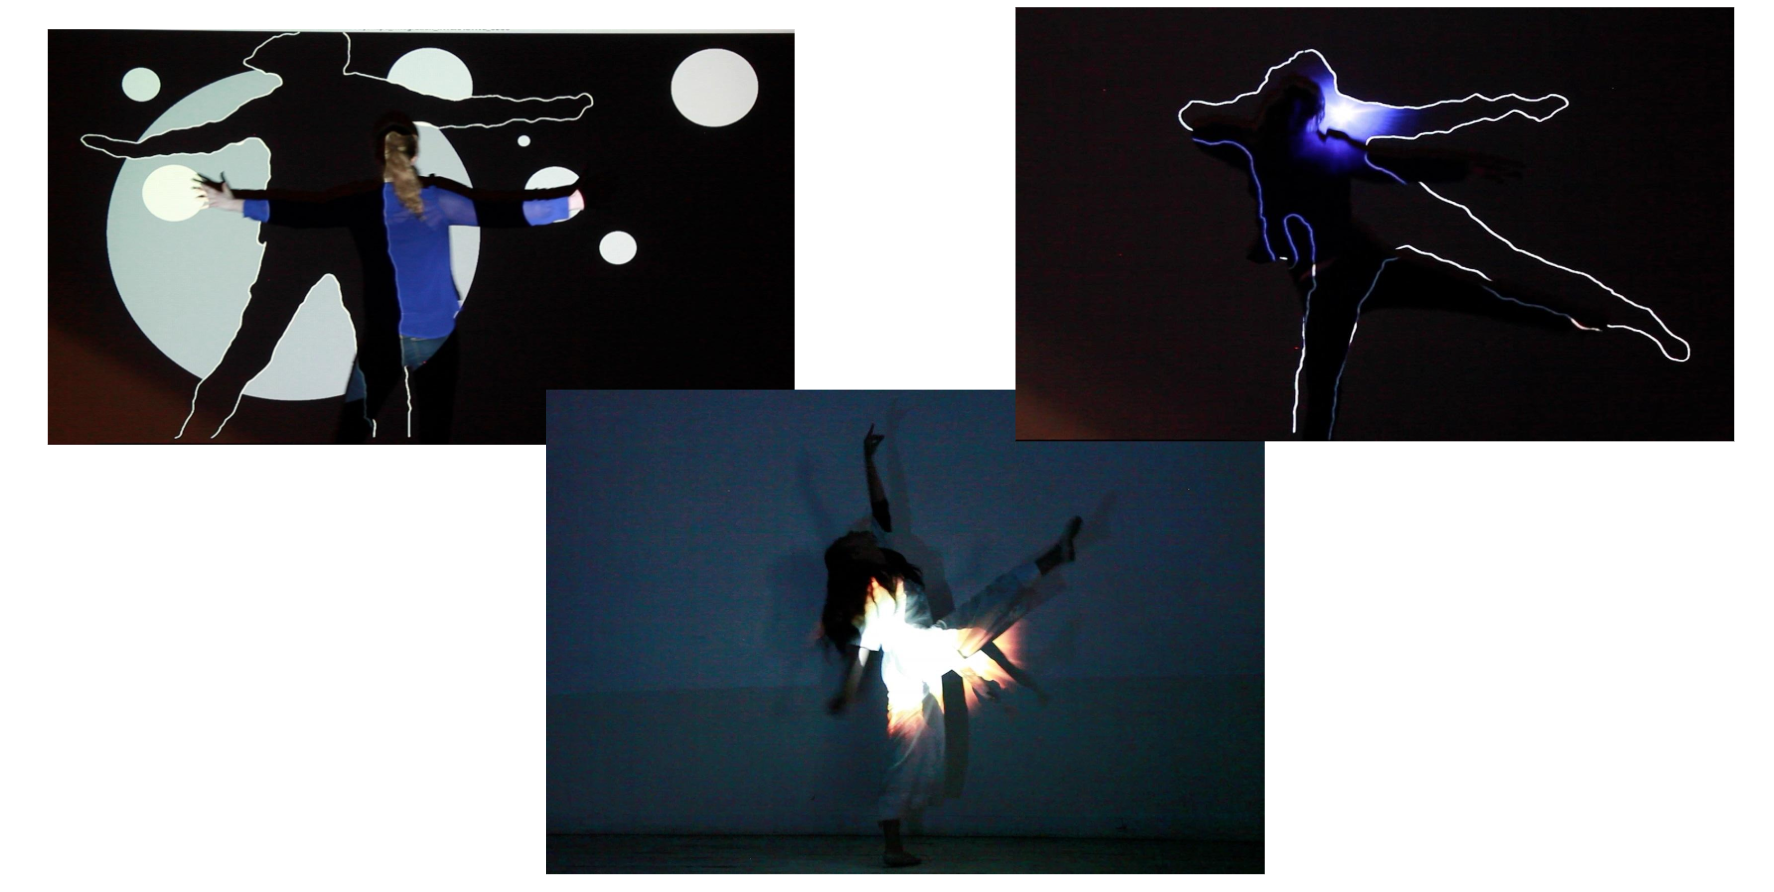
\includegraphics[width=.8\linewidth]{figures/bg1.png}
        \label{fig:sub-first}
    \end{subfigure}
    \begin{subfigure}
        \centering
        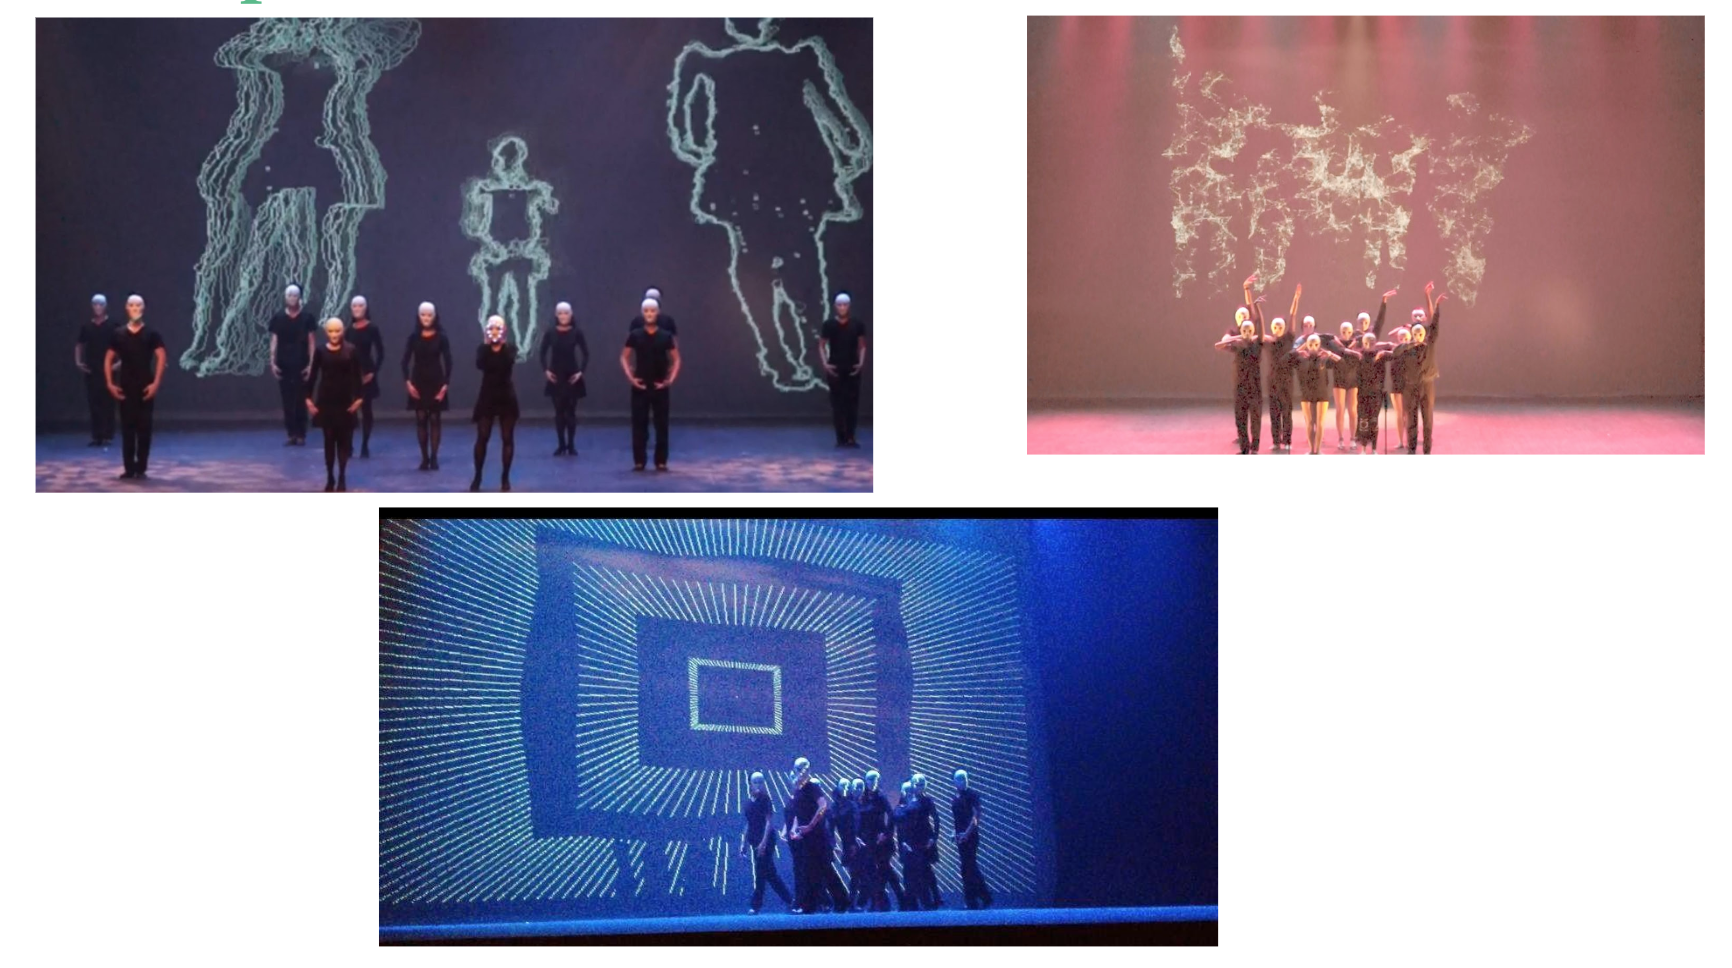
\includegraphics[width=.8\linewidth]{figures/bg2.png}
        \label{fig:sub-second}
    \end{subfigure}
    \caption{Artistic show produced by ISS}
    \label{fig:bg}
\end{figure}

\begin{figure}
    \begin{center}
        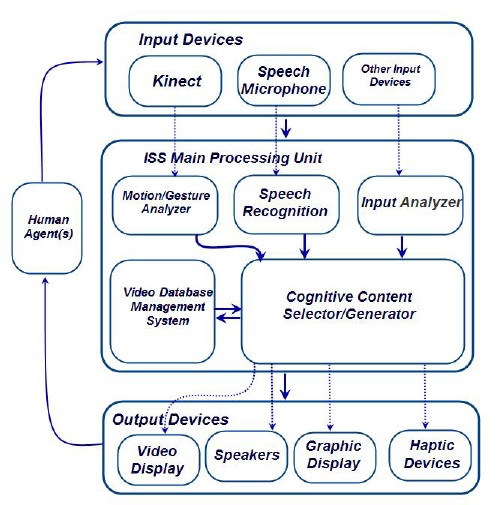
\includegraphics[scale=0.6]{figures/iss_v2_model.png}
    \end{center}
    \caption{Block Diagram of Illimitable Space System}
    \label{fig:iss-v2}
\end{figure}

ISS (Illimitable Space System) is a real-time interactive configurable
artist's toolbox used to create music visualizations, visual effects and
interactive documentary based on the inputs from users such as gestures or
voice.
The goal of ISS is to enhance interaction between actors and graphics so that
it is all projected as an integrated piece. It aims at freeing up the artists
as much as possible so that they are able to perform freely in their own way
without worrying about the performance technology.
ISS was originally proposed in~\cite{first-proposed-iss} and improved 
in~\cite{iss-v2-design-theory-journal}, in order to differentiate them, we named
the former ISSv1 and the latter ISSv2. Also, there was 
ISSv3~\cite{iss-v3-appy-hour-gem2015, iss-v3-appy-hour-siggraph2015} which
was designed for virtual reality application, but out of this thesis scope. We
mainly focus on ISSv2 which can be conceptually represented by~\autoref{fig:iss-v2}, 
which is a significant improvement in ISSv1 and is used
for rapid development of real-time, motion-based graphics applications
implemented in Processing which is on top of Java.

\section{Limitations of ISSv2}
\label{sec:intro-lim-issv2}

When we have more chances to do different performances in different places,
we found that sometimes the stage given to us is too large and cannot be covered
by only a single camera. It restricts us to design the performance within a
limited space, which is actually conflicting with our project's name, Illimitable Space
System.
Also, recently the price of consuming level depth camera has become
much cheaper. In the market, there are different kinds of depth cameras
being manufactured (like Kinect v1, Kinect v2 and RealSence) and these cameras
become more and more powerful (higher speed, frame rate, resolution, larger
bandwidth and etc). But ISSv2 is hardware-dependent can only work with Kinect
v1 which is kind of out of date now.

Under such a situation, we started to think that if one camera is
not enough, we can have more than one and each of them takes care of a certain
area of the large stage so that we break the restriction and can design much
better performance without space limitation.
By using more than one camera, a problem comes to our mind naturally: How can
we identify the same person across different cameras since we need to track them
and apply specific visual effects on certain actors?
From this point, developing a system that can track people through multiple
cameras becomes essential.
This idea can not only benefit us but also the security-and-protection industry
or even the police department. Since with such a system, you can identify a
specific target (like suspect) across multiple cameras if you have captured it
in any one of your cameras.

In order to catch up with the device evolution, we would like to move from 
older devices to the latest models. But we don't want to discard our previous 
compatibility while evolving to new technologies. So how to enable our previous work to be 
compatible with various kinds of cameras is also a challenge for us.

%\section{Problem Statement}
\section{Research Problem}
\label{sec:intro-pbstat}

%In order to address the limitations we found for ISSv2, our research can be

From the situation we described above, our research can be
intuitively divided into two parts: 
(1) person re-identification and
(2) depth camera abstraction.
Person re-identification (ReID) recently is a hot research topic in the
computer vision community. It requires the system to identify the same person
across different cameras, which can be broken down into three components:

\begin{itemize}
    \item person detection
    \item person tracking
    \item person retrieval
\end{itemize}

If we have a fast enough system, we don't explicitly need person tracking.
Instead, we perform person detection on each coming frame from the camera which
is functionally equivalent to person tracking. Under this consideration, we
omit person tracking in this thesis.
For device encapsulation, we  currently focus on the total of three kinds of
cameras: Kinect v1, Kinect v2 and RealSense D435 and we also make sure that when
a new device needs to be appended, the process will be simple and
implementer-friendly as well as having no side-effect with the existing devices.

In the following subsections, we are going to formulate our
research problem scientifically. For person detection, we enlarge our target
set not only on the person but for all kinds of objects and the same applies to
person retrieval. So we end up with object detection and object retrieval.

\subsection{Object Detection}

In object detection, you are given an image $I$ and a list of classes $C$ which
the objects
appear in $I$ belong to. Your task is to detect instances of the object within
$I$ belong to a specific class in $C$.
For each instance $i$, you need to output first $c \in C$ which represents which class
this instance belongs to and second
a bounding box $B$ to indicate the location of that instance with respect to the
image $I$.

\subsection{Object Retrieval}

In object retrieval, you are given a query image $q$ and a set of gallery images
$G$. Your task is to find the
most likely image $g \in G$ for which both $q$ and $g$ represent the same instance
$instance(q) = instance(g)$.

\subsection{Device Abstraction}

The second part we mentioned above is that we try to conceptually eliminate the differences
among various kinds of cameras. It can be translated as we would like to access
data via a set of common APIs without considering what kind of hardware
we are using. Assume we have a list of device $D = {d_1, d_2, ..., d_n}$ and a
list of API $F = {f_1, f_2, ..., f_n}$,
we can trigger the same effect
while calling the same API which can be mathematically expressed as:
$
\exists f_n \in F, \forall (d_i, d_j) \in D
\Longrightarrow f_{n}(d_i) = f_{n}(d_j)
$

\section{Motivation and Goal}
\label{sec:intro-mot-goal}

The original design of ISSv2 targets to create music visualization, visual
effects and interactive documentary easily for artistic people who don't have 
extensive knowledge in computer science and programming. So the architecture and
the design needs to be relatively simple. The main focus should be given to visual effect
design and how to display them to the audiences.
What's more, currently, ISSv2 can only use Kinect v1 as the input device. Efforts have
been put to enable Kinect v2 but due to the low-level dependencies (e.g.
hardware driver) conflict, not all the features can be replicated and compatible.

Based on the limitation we found and some new demands,
we conducted a comprehensive survey and found that there is no existing solution
targeting our problem directly.
So we would like to abstract a back-end system for ISS while keeping the
front-end remaining unchanged. The back-end system here means the hardware,
scheduling algorithm, pipeline construction, and other common APIs. Front-end
basically means the artistic part, like visual effect design, music
visualization and so on.

It is worthwhile to mention that as this work is being developed, there are
another two other research works going on in parallel under the same umbrella.
Jashanjot Singh is working on a system that can do gesture tracking and
recognition while Yiran Shen is working on a system that can do facial
landmarks detection and facial expressions recognition. We would also like
these two works to be accessed via the same set of APIs which means all these
three works should somehow be operated within the same operational software
framework.

Up to now, we should be able to summarize our goal:
\textbf{
    we would like to design and implement a system that provides a way to
	abstract different kinds of depth cameras and the functionality of person
	re-identification. It should also leave space for other modules to be
	integrated with good extensibility and usability.
}

\section{Scenario and Requirement}
\label{sec:intro-scen-req}

With the goal we defined above, in this section we will give a few concrete
use-case scenarios we expect to achieve from the final production of this thesis.
These scenarios, in their own way, highlight one or more problems that have not
been solved by any existing solution yet. We not only aim at solving these problems
individually, but also to provide a general solution to all these problems
under the same software solution.
We analyze these scenarios one by one, then extract both functional and
non-functional requirements, which becomes the concrete implementation goal of
our solution.

\subsection{Device Switch and New Device Addition}
\label{sec:intro-sq-dev}

Imagine a scenario where we would like to develop a new version of ISS
may be named ISSv4. This time, we need to support device $D_1$ and $D_2$ where
$D_1$ was supported by its previous version and $D_2$ is a newly added device.
The difference between $D_1$ and $D_2$ is that $D_1$ was designed for the indoor
environment while $D_2$ can perform better in the outdoor environment. So depending on
where the performance will be given, we need to be able to switch between $D_1$
and $D_2$. This kind of switch should just literally unplug one device from
the system and plug in the other one. Only a few or even no modifications should
be made in the code to obtain the same effect from the application point of
view. Also, if later a new device $D_3$ comes to the market, the system
should be easily extended to be able to make use of $D_3$.

This usage scenario can be abstractly summed-up as the following, which becomes
two of our requirements:

\begin{itemize}
    \item \textbf{FR1}: The solution shall provide an abstraction layer for the
    hardware that enables the physical device transparency property to
    the users.
    \item \textbf{FR2}: The solution shall ensure the extensibility of the
    abstraction layer required in \textbf{FR1} which means when the new devices
    come only a few or no modification need to be made and will not affect the
    existing system.
\end{itemize}

\subsection{Back-end Abstraction}
\label{sec:intro-sq-abs}

Let's continue using the scenario setting we described above, this time we need
to map the performance onto another backdrop rather than the one where the
actual performance is taking place, which means that we need to extract only
the actors out with all the other background removed. Keep in mind that
there are two different devices supported $D_1$ and $D_2$, according to our
settings. The most straightforward way to do is that for each device, we
create a filtering algorithm employing some methods provided by the hardware
driver to perform background removal. But the limitation is also obvious when
a new device is added: you have to re-implement the same algorithm again and
again for each new device. If another demand is required, you need to implement all of them when a
new device is being supported.
Another elegant solution is that we could extract the data needed to perform
background subtraction into a common data structure then apply a general
algorithm based on it. Next time, when a new device comes, what we need to do
will be just the transformation from the device-specific data structure to our
common one. If some other demands like background removal are required, we can
always follow the same pattern to solve them. We call all these common data structures
and common algorithms the back-end of the system.

This usage scenario can be abstractly summed-up as the following, which becomes
one of our requirements:

\begin{itemize}
    \item \textbf{FR3}: The solution shall be able to serve as a back-end of the
	existing ISS system providing a set of commonly used data structures and
	functionalities for reusability.
\end{itemize}

\subsection{Person Re-identification}
\label{sec:intro-sq-reid}

Imagine a scenario where there is a show given by two actors, and we would like to
project visual effect $\mathit{vfx}_1$ on actor $a_1$ while $\mathit{vfx}_2$ on
actor $a_2$.
Unfortunately, the stage is too large and cannot be covered by a single camera.
We have to employ two cameras, each of them covers half the space of the stage.
According to the performance director, we need to make sure that no matter
where these two actors are, the visual effects have to be mapped properly.

This usage scenario can be abstractly summed-up as the following, which becomes
one of our requirements:

\begin{itemize}
    \item \textbf{FR4}: The solution shall be able to detect all the appearance 
    of human bodies and provide their location by bounding boxes.
    \item \textbf{FR5}: The solution shall be able to recognize a cropped image 
    with an identity across multiple cameras if the identity has been defined in 
    advance.
\end{itemize}

\subsection{Skeleton Tracking}
\label{sec:intro-sq-skt}

In ISSv2, we have some visual effects designed specifically for the human 
skeleton. But because of the underlying dependencies issue, we can only obtain 
the skeleton data from Kinect v1 camera.
In order to break the restriction from the specific device-oriented
dependencies, we need to make the skeleton extraction process 
device-independent.
It means we should be able to extract skeleton data from a variety
of devices and convert them into the common skeleton data format which is simply 
a set of points in a picture. A possible scenario can be described as the following: a
performance director would like to make use of some skeleton-based visual
effect and want them to be used with different devices.

This usage scenario can be abstractly summed-up as the following, which becomes
one of our requirements:

\begin{itemize}
    \item \textbf{FR6}: The solution shall provide the functionality to enable
    users to perform skeleton tracking among various kinds of cameras.
\end{itemize}

\subsection{Interaction with Other Modules}
\label{sec:intro-sq-inta}

As mentioned before, there are a gesture and facial recognition modules being developed
concurrently to our research. Theses modules should be able to use the infrastructure (e.g.
device abstraction) we proposed in this thesis. Also the module we develop here
should be able to communicate with these two other modules from other system
developers. Imagine a scenario where the visual effect needs to change according
to the actor's gestures. When the actor push their hand, a zoom-out
effect should be applied while the actor pull their hand, a zoom-in effect
occurs.

This usage scenario can be abstractly summed-up as the following, which becomes
one of our requirements:

\begin{itemize}
    \item \textbf{FR7}: The solution shall provide fundamental infrastructure
    for other modules to use and vice versa. It shall enable an abstract 
    communication infrastructure common to all developed modules.
\end{itemize}

\subsection{Non-functional Requirements}
\label{sec:intro-non-func-req}

By analyzing the scenarios we described previously, we found that in order to
achieve them our solution must meet the following non-functional requirements:

\textbf{Extensibility:}
\textit{The ability of a software system to acquire and integrate new
components.}

As the devices will become more and more multitudinous and the algorithms for
person re-identification will be more and more advanced, it becomes essential
to design a solution with great extensibility that later on we still
be able used to add or integrate more devices and algorithms into our existing
solution smoothly and easily.

\textbf{Usability:}
\textit{The ability of a software system to effectively provide the expected
functionalities to the user, in a manner that is as intuitive and the least
strenuous or
problematic as possible.}

For any kind of software system, in order to attract the users and/or programmers, as the designer
we should try our best to provide simple, meaningful and understandable APIs.
That means the name of our APIs, the required parameters for each functionality
and the final result from the return value should be concise, compact and
logically make sense. For the experienced users in the same area, they should
be able to move from other similar solutions to ours without putting too much effort.
In other words, the learning curve should be as smooth as possible
and necessary documentation and comments should be provided properly.

\section{Contributions}
\label{sec:intro-contrib}

Our contribution are four-fold:

\begin{itemize}
    \item We offer an overall architecture that allows users to perform
    real-time skeleton tracking, person detection, and person
    re-identification.
    
    \item We offer a way in general that can allow the user to access
    different depth cameras within the same set of APIs with good extensibility.
    
    \item We offer a way to allow cross cameras tracking with a pluggable
    detector and recognizer.
    
    \item We offer a pipeline execution mechanism to allow the user to assemble 
    various components to form their application without knowing the underlying 
    details.
    
    \item We offer a way for the researcher to enable person re-identification
    experiment on top of TensorFlow and Keras.
\end{itemize}

\noindent To achieve the above, we implemented the following features:

\begin{itemize}
	\item Design and implement a modular framework solution which consists of
	the core and specialized frameworks that enable real-time skeleton 
	tracking, person detection, and person re-identification.

    \item Design a device module that encapsulates the depth cameras from
    different brands with good extensibility. Instantiate this module to
    support three kinds of physical devices.
    
    \item Design and implement a pipeline module that provides a linear
    execution mechanism over a series of filter that each encapsulate a 
    specific transformation step.

    \item Design a detector specialized framework and instantiate it for
    person detection task with a deep learning-based algorithm named YOLO.

    \item Design a recognizer specialized framework and instantiate it for
    person re-identification using the deep learning-based identification and
    triplet models.

    \item Use the general framework solution to build several commonly used
    applications like camera calibration, green screen image, and image
    alignment.

    \item Implement an abstraction layer for deep learning-based person
    re-identification dataset to allow training and validation among multiple
    dataset easily.
\end{itemize}

%\section{Methodology}
%\label{sec:intro-methodology}

\section{Thesis Outline}
\label{sec:intro-outline}

In this chapter, we introduced our research background, pointed out the
existing limitations, and stated the research problems giving them clear academic
definitions and restricted our scope.
In the following chapters, the thesis will be structured in the way listed
below:

\begin{itemize}
    \item In \autoref{chap:RelatedWork}, we will review existing literature
    related to our research problem and also the available software which is
    useful for our implementation. In the summary section of this chapter,
    based on our need, we will select our target detector and recognizer and
    stick with them in our implementation described in the following chapters.

    \item In \autoref{chap:fw-design} and \autoref{chap:fw-inst}, with all
    needed background in hand from the previous chapter, we will propose our
    solution in detail and explain our design and implementation in a top-down
    manner.

    \item In \autoref{chap:fw-app}, we will describe the applications built on
    top of our proposed solution, which becomes a proof of concept that our
    solution can actually fulfill our functional requirements.

<<<<<<< HEAD
    \item In \autoref{chap:Evaluation}, we will report our results showing the
	benchmarks for the main components in our solution with commonly acknowledged 
	metrics. Also, we will prove that both functional and non-functional
    requirements are really fulfilled.
=======
    \item In \autoref{chap:Evaluation}, we will first demonstrate both the
    functional and non-functional requirements are really fulfilled by our
    framework solution. Then we report our result showing the benchmark for the
    main components in our solution with commonly acknowledged metrics.
>>>>>>> 8a860f413a6d6a177b30d175dd449d3f0ea1566b

    \item In \autoref{chap:Conclusion}, we sum up our work with advantages and
	limitations and point out some potential research directions in the future.
\end{itemize}

%In the following chapters, we will first describe the existing solution of our
%interested research and review corresponding literature in
%\autoref{chap:RelatedWork}
%so that we can see the gap and understand the current state of the art in this
%domain.
%With all needed background, we then will propose our solution in detailed and
%explain our design and implementation in a top-down manner in
%\autoref{chap:fw-design} and \autoref{chap:fw-inst}. Followed by the
%application we built on top of our solution to address the cross cameras
%tracking problem \autoref{chap:fw-app}.
%In \autoref{chap:Evaluation}, we will report our result showing benchmark for
%each components in our solution with commonly acknowledged metrics.
%At the end, we sum up our work with advantages and limitations, pointing our
%some potential directions for future work \autoref{chap:Conclusion}.

% EOF

\chapter{Related Work}
\label{chap:RelatedWork}
\index{Related Work}

%%%%%%%%%%%%%%%%%%%%%%%%%%%%%%%%%%%%%%%%%%%%%%%%%%%%%%%%%%%%%%%%%%%%%%%%%%%%%%%%

As per discussed in the previous chapter, we split our work into two parts:
(1) person re-identification (2) device abstraction.
In this chapter, we are going to introduce the background for each part. For the
person re-identification part, we will review the literature from object
detection and person re-identification, which the former is the prerequisite of
the latter. For the device abstraction part, we are going to examine currently
available software which may become useful for our objective and be adopted as
dependencies in our solution.


\section{Object Detection}
\label{sec:related_work_obj_det}

Object detection is one of the fundamental tasks in computer vision research,
which is a natural extension of the classification problem requiring to detect 
the presence of objects and accurately locate them within the given image.
This subject has been explored by many researchers along the time and a lot of
detailed surveys have been conducted 
\cite{survey1-on-dl-od-2018, survey2-on-dl-od-2018}.
We can observe from \autoref{fig:od-timeline}, since 2012 the deep
learning-based approaches dominated the object detection domain.
In this section, we are going to review the two classes of literature in object
detection based on deep learning methods (detailed explanation will be given as
subsection for each of the items listed below).

\begin{itemize}
    \item Two stages approaches
    \begin{itemize}
        \item R-CNN
        \item SPP-net
        \item Fast R-CNN
        \item Faster R-CNN
        \item Mask R-CNN
    \end{itemize}

    \item One stage approaches
    \begin{itemize}
        \item YOLO v1, v2 and v3
        \item SSD
    \end{itemize}
\end{itemize}

\begin{figure}
    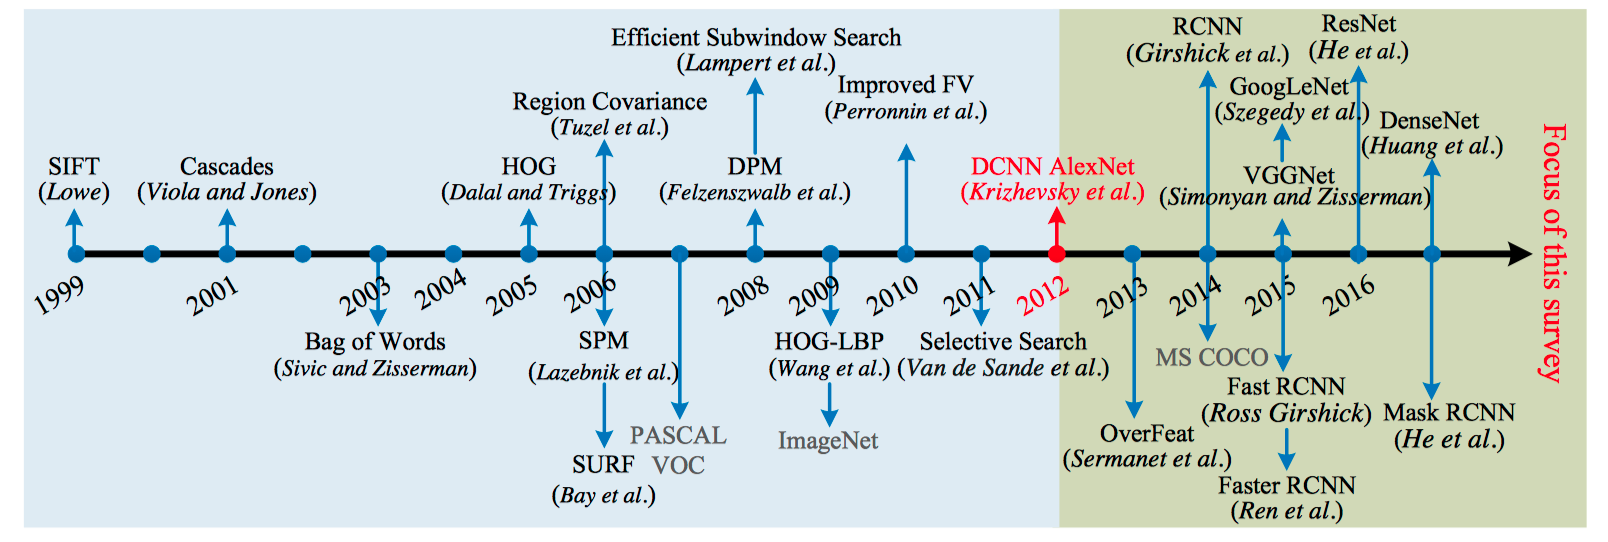
\includegraphics[width=\linewidth]{figures/timeline_od.png}
    \caption[Timeline of various methods proposed for object detection]
    {Timeline of various methods proposed for object detection
    ~\protect\cite{survey1-on-dl-od-2018}. The methods in blue area are the
    hand-crafted detector and the methods in green area are the deep
    learning-based approaches.}
    \label{fig:od-timeline}
\end{figure}

The world ``stage'' here means an independent process or a separate branch
within the deep neural network structure.
As their names imply, one stage approach finish the whole object detection
process in one shot indicating it will be faster than its two stages sibling
due to the fact that less computation being performed.
While the two stages approach has an independent process to propose the areas
where it may contain an object then perform detection on those places. The
presence of the area proposed stage takes more time but since it is elaborated
and can cover more potential area than the one-stage approach, it can gain
better results in the context of accuracy.
%As their names imply, one stage approach finish the whole object detection
%process in one shot indicating that it is faster but due to less computation
%the accuracy is less than the two stages approach which takes more time
%because
%it has an independent process to propose the areas where it may contain an
%object then perform detection on those places but can gain higher
%accuracy.
Determine to use which kind of detector depends on the realistic
requirement of the application. In this thesis, since we have real-time response
as non-functional requirement, one stage detector will be definitely a better 
choice. 
%and we mainly focus on the YOLO v3 detector, the implementation detail will be 
%explained in the next chapter.

\subsection{Two Stages Detector}
\label{sec:related-worked-two-stages-detector}

Most of the two stages detectors follows the same methodology. Firstly,
proposes a bunch of candidate regions that may contain object(s) then using a
convolutional neural network (CNN) to extract feature descriptors of each
region.
Finally, feed the descriptor into a classifier to figure out what kind of 
object they are, if exist, and fall into which bin of the pre-defined
categories.

\subsubsection{R-CNN}

R-CNN was the seminal work of employing CNN on object detection task, at that
time it was proposed, it boosted the accuracy from 35.1\% to 53.7\% on PASCAL
VOC dataset \cite{r-cnn-paper-2013}.
It designed a cascade pipeline contains four modules shown as
\autoref{fig:r-cnn}, named R-CNN stands for region with CNN features.
There are two important points this work brought to the table:
(1) it proposed a selective search 
\footnote{Selective Search is a region 
proposal algorithm used in object detection. It is designed to be fast with a 
very high recall. It is based on computing hierarchical grouping of similar 
regions based on color, texture, size and shape compatibility.} 
method to find the possible candidates
replacing the old fashion sliding window way,
which improve the computation time significantly.
(2) it adopted CNN as feature extractor which can obtain more robust
features rather than the hand-crafted one.

\begin{figure}
    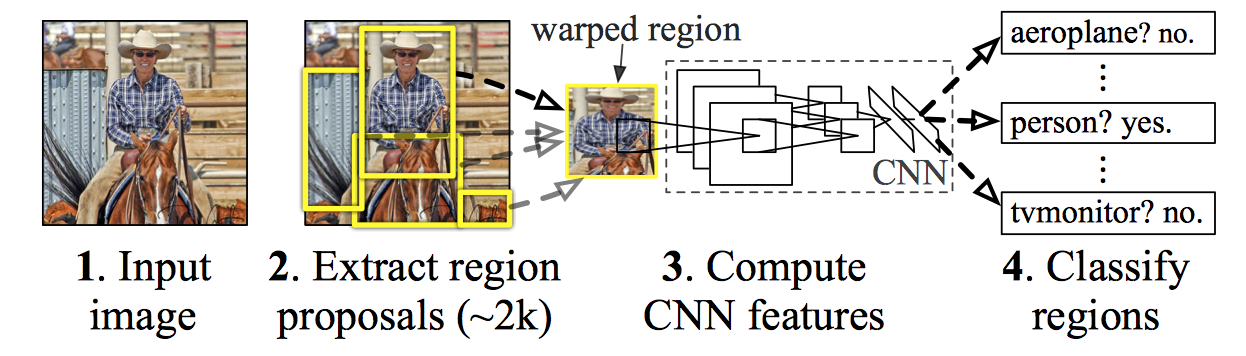
\includegraphics[width=\linewidth]{figures/r_cnn.png}
    \caption{R-CNN system overview ~\protect\cite{r-cnn-paper-2013}.}
    \label{fig:r-cnn}
\end{figure}

\subsubsection{SPP-net}

Even though R-CNN brought large margin of improvement into the object detection
research, it still has the potential to be better observed by Kaiming He and
his team. They proposed spatial pyramid pooling network (SPP-net)
\cite{spp-net-paper-2014} one year after R-CNN being published. It improved
both runtime efficiency and accuracy compared to R-CNN.
They identified two main issues in R-CNN solution:

\begin{itemize}
    \item The generated candidate regions are easy to have overlap among each 
    other which can lead to repeated computation of the same feature maps.

    \item When ensuring the input image to a fixed size by no matter cropping or
    warping. They both have a large possibility that leads to information
    missing which can affect the training significantly.
\end{itemize}

SPP-net solved the first problem by reversing the order of selective search and
convolution operation.
It also employed a special layer named ``spatial pyramid pooling" at the
end of the convolutional layer to eliminate the second problem, that is how its 
name comes from.
By using SPP-net, the final feature maps will only be
computed once and features will be pooled in arbitrary regions to generate 
fixed-length descriptor for training, shown as \autoref{fig:spp-net}.


\begin{figure}
    \begin{center}
    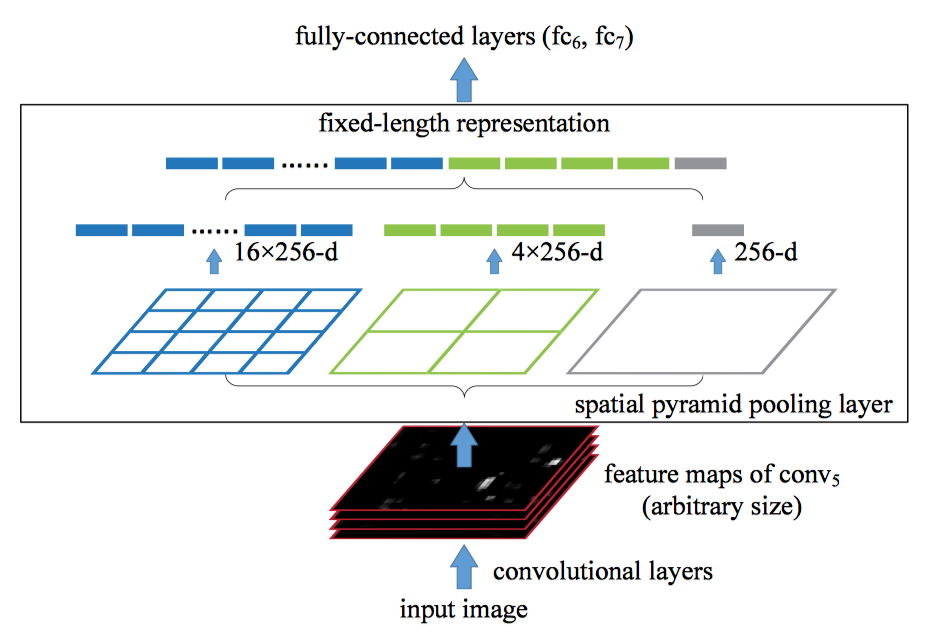
\includegraphics[scale=0.7]{figures/spp_net.png}
    \end{center}
    \caption{Illustration of how spatial pyramid layer works
    ~\protect\cite{spp-net-paper-2014}.}
    \label{fig:spp-net}
\end{figure}


\subsubsection{Fast R-CNN}

Fast R-CNN \cite{fast-r-cnn-paper-2015}, just like its name says, is
an advanced version of R-CNN, created by the same author Ross Girshick 
independently. This update mainly focuses on speeding up both
training and testing procedures. It targeted
at not only R-CNN but also SPP-net for their common drawbacks:

\begin{itemize}
    \item The training pipeline is a multi-stages process.
    \item Features are written to disk during training.
    \item The inference phase is too slow.
\end{itemize}

The solution for these issues is quite straight forward. Firstly, the author
changed the cascade pipeline to become a parallel one, shown as
\autoref{fig:fast-r-cnn}. 
Secondly, it modified the loss to be a multi-task loss which reduces the
training complexity and makes all the layers updatable (the proposed fine-tuning
algorithm cannot update the convolutional layer that precedes the spp layer).
Thirdly, the features cached on the disk were no longer needed.

\begin{figure}
    \begin{center}
    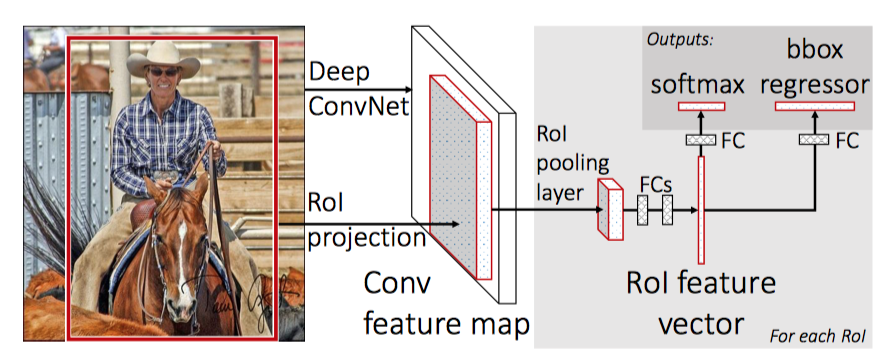
\includegraphics[scale=0.7]{figures/fast_r_cnn.png}
    \end{center}
    \caption{Parallel workflow of Fast R-CNN
    ~\protect\cite{fast-r-cnn-paper-2015}.}
    \label{fig:fast-r-cnn}
\end{figure}


\subsubsection{Faster R-CNN}

Faster R-CNN \cite{faster-r-cnn-paper-2015} was a milestone of the usage of 
deep convolutional neural network in the research of object detection. It was 
created by the combination of the teams which proposed R-CNN and SPP-net.
Before it came up, the candidate regions were calculated via a method called 
selective search. 
But in this case, they introduced a region proposal network (RPN) which was 
embedded as a branch into the model can learn how to
produce reliable candidate regions during the training time, the overall
structure of Faster R-CNN shown as \autoref{fig:faster-r-cnn}.
By using such an architecture, the model can achieve predicting bounding box of 
the object and computing the objectness score simultaneously (through one 
forward pass). There are several advantages of Faster R-CNN compared to its 
previous works:

\begin{itemize}
    \item Deep learned features are more reliable than the selective search one.
    \item The whole network can be trained end-to-end \footnote{The learning 
    that optimizes the network weights by considering the inputs and outputs 
    directly is called end-to-end learning. }.
    \item The whole pipeline can be done on GPU (selective search need to be
    done on CPU before) which can speed up the training time.
\end{itemize}

\begin{figure}
    \begin{center}
        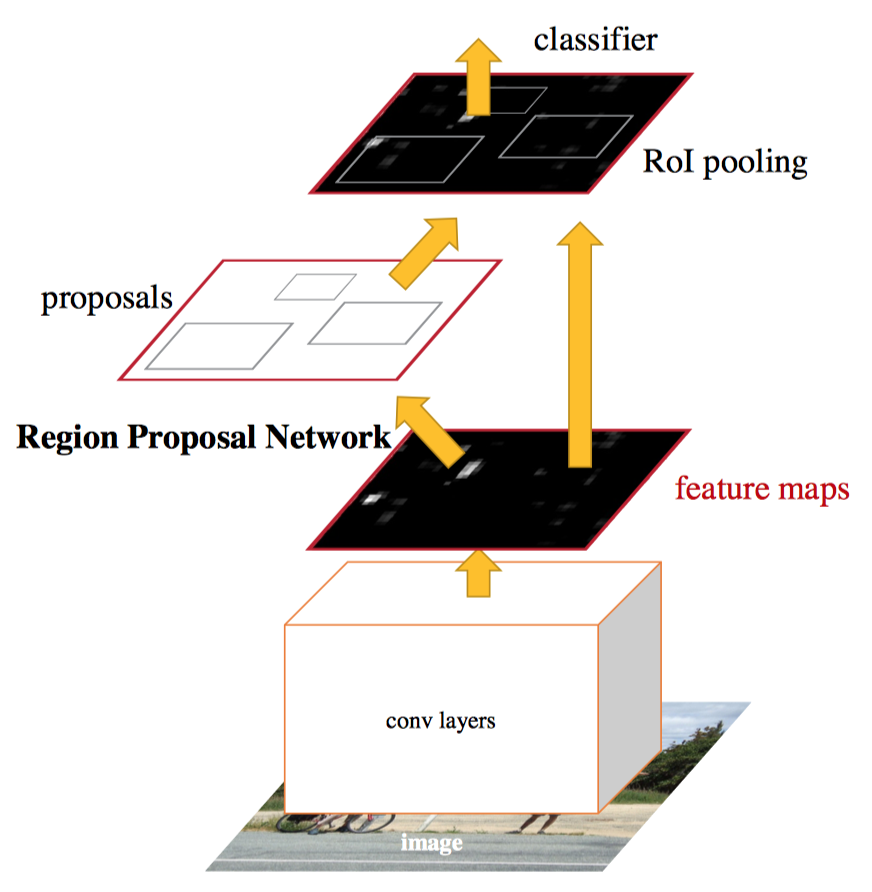
\includegraphics[scale=0.5]{figures/faster_r_cnn.png}
    \end{center}
    \caption{Structure of Faster R-CNN ~\protect\cite{faster-r-cnn-paper-2015} 
    network.}
    \label{fig:faster-r-cnn}
\end{figure}

There is one more thing needs to be pointed out, this work introduced the
concept of ``anchor'' which has been widely
used in the latter objection detection research including the one stage
detector we are going to review in the next subsection.
At each sliding-window position, the network would simultaneously predict $k$
region proposals which relative to
$k$ reference bounding boxes, these reference boxes are called anchor, one example
can be shown as \autoref{fig:anchor}.

\begin{figure}
    \begin{center}
    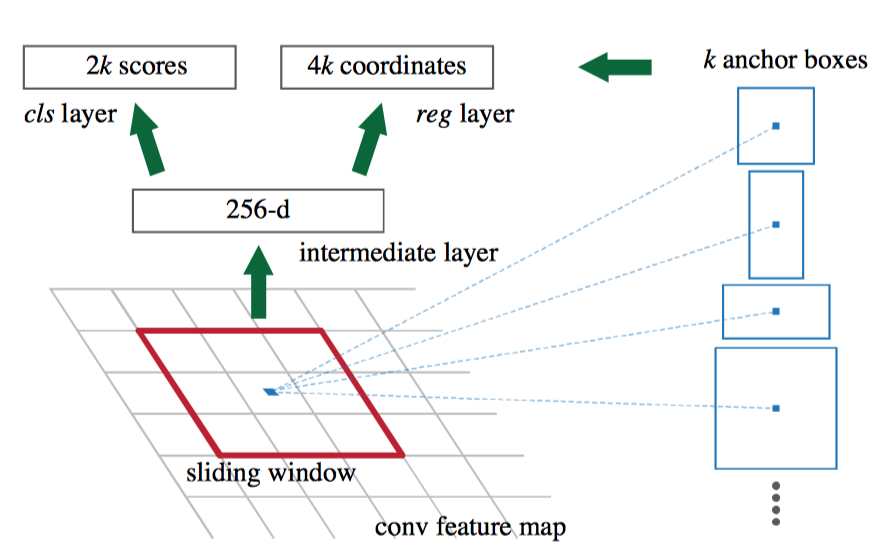
\includegraphics[scale=0.6]{figures/anchor.png}
    \end{center}
    \caption{Illustration of the anchor mechanism
    ~\protect\cite{faster-r-cnn-paper-2015}.}
    \label{fig:anchor}
\end{figure}


\subsubsection{Mask R-CNN}

The most recent work of the R-CNN-based research was called Mask
R-CNN \cite{mask-r-cnn-paper-2017} proposed
by Kaiming He again. It was not only an object detection network but also can be
used in the object segmentation domain. The idea
was that (1) it added another mask branch into the network to create a mask for
each detected object instance and (2) using a
more advanced backbone network for feature extraction (e.g. ResNet and FPN).
Its architecture shown as \autoref{fig:mask-r-cnn}.
Again, the loss used to guide the training is the multi-task loss from Faster
R-CNN with the mask loss added expressing as:
$L = L_{cls} + L_{bbox} + L_{mask}$. Another creative idea, ROI alignment, is
notable to mention which can improve accuracy for bounding boxes regression.

\begin{figure}
    \begin{center}
    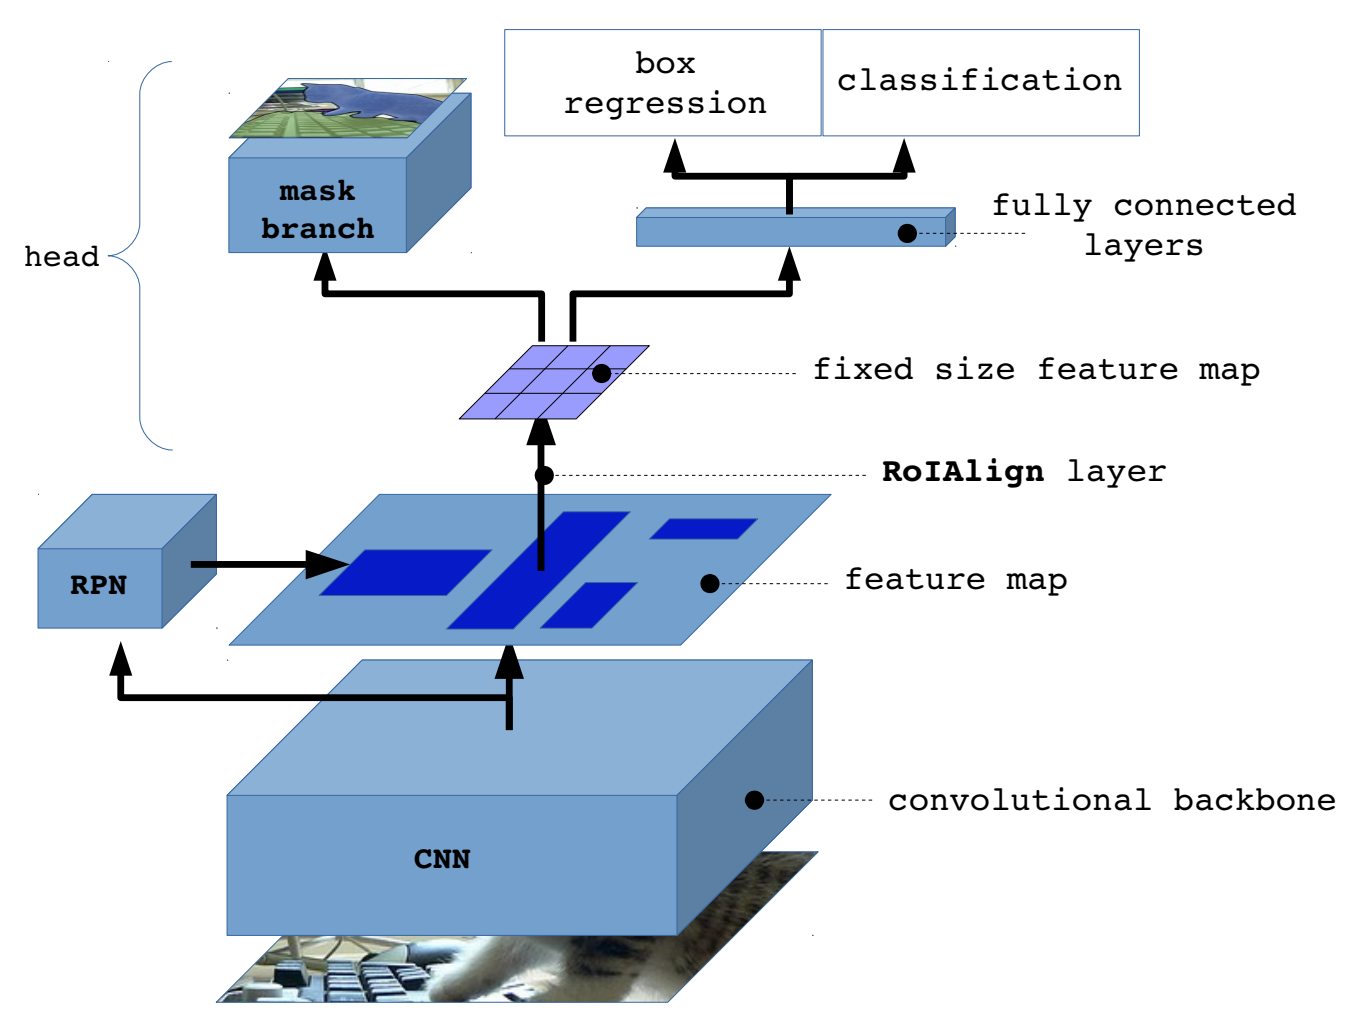
\includegraphics[scale=0.5]{figures/mask_r_cnn.png}
    \end{center}
    \caption{Architecture of Mask R-CNN ~\protect\cite{mask-r-cnn-slide}.}
    \label{fig:mask-r-cnn}
\end{figure}


\subsection{One Stage Detector}
\label{sec:related-worked-one-stage-detector}

One stage detector refers to those who directly predict class score and bounding
box offsets from the input with a single feed-forward CNN network. There is no
separate region proposed process exists at all, all the computations are done
within just a single network which can be optimized end-to-end directly on
detection performance.

\subsubsection{YOLO}
\label{sec:related-worked-yolo}

YOLO stands for ``you only look once'', which indicates it is an one-stage
object detector. Until now, there is total
three versions of the YOLO algorithm. They are YOLO v1, YOLO v2, YOLO v3 which 
were published in 2015, 2016, 2018 respectively. 
Compared with the R-CNN series, YOLO doesn't have the stage of 
candidate region calculation. It uses a single network to
directly compute the objectness score and regress the bounding
boxes if objects exit.

\textbf{YOLO v1} \cite{yolov1-paper-2015}, this work is the fundamental
building block. The latter YOLO's algorithm
just borrowed or added advanced techniques or tricks to improve the
performance. The workflow of the algorithm can
be summarized as the following steps and visualized as
\autoref{fig:yolo-v1-workflow}:

\begin{itemize}
    \item Take the input image (with size $448 \times 448$), cut it into $S
    \times S$ grids, each of them is responsible for detecting those objects
    whose center located within this grid.

    \item Each grid will predict $B$ (an integer) bounding boxes and the
    confidence score of each box. For each predictive bounding box, the result
    should be a five-dimensional vector $(x, y, w, h, c)$ representing the 
    center location of the box $(x, y)$, the width and height of the box $(w, 
    h)$, and the confidence socre $c$.

    \item For each grid (no matter how may bounding box is required), it should
    also output a probability for all required classes (if the dataset contains
    10 classes of object, it should output a probability for each class which
    means 10 probabilities in total).

    \item Sort all the result according to the score and use a threshold to 
    filter out the detected bounding boxes whose probability lower than it.
\end{itemize}

\begin{figure}
    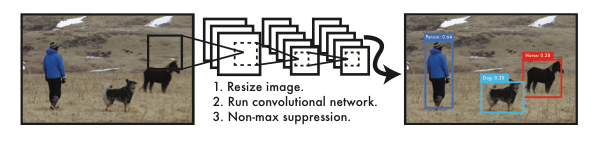
\includegraphics[width=\linewidth]{figures/yolo_v1_workflow.png}
    \caption{Workflow of YOLO v1 ~\protect\cite{yolov1-paper-2015}.}
    \label{fig:yolo-v1-workflow}
\end{figure}

An example process for an input image can be shown as
\autoref{fig:yolo-v1-example}, from that figure we can find that the
class score computation and bounding box prediction happened parallel. At
the end, another common technique, non-maximum
suppression \cite{non-maximum-suppression-paper} was applied to eliminate the
highly overlapped boxes but point to the same object.
In the implementation point of view, the YOLO series was written in pure C from
sketch, the author provided his own deep learning framework
named Darknet \cite{darknet13} which includes
backbone network, optimizer, parameters update
methods, etc. The backbone network's architecture is shown as
\autoref{fig:yolo-network}, which is a 24 convolutional layers network
with 2 dense layers appended. The whole model was pre-trained on ImageNet
using image with resolution $224 \times 224$ then doubled the size for
detection.


\begin{figure}
    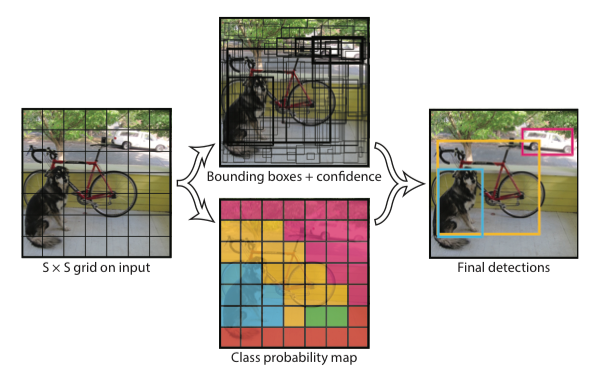
\includegraphics[width=\linewidth]{figures/yolo_v1_grid_example.png}
    \caption{An process example YOLO v1 ~\protect\cite{yolov1-paper-2015}.}
    \label{fig:yolo-v1-example}
\end{figure}

\begin{figure}
    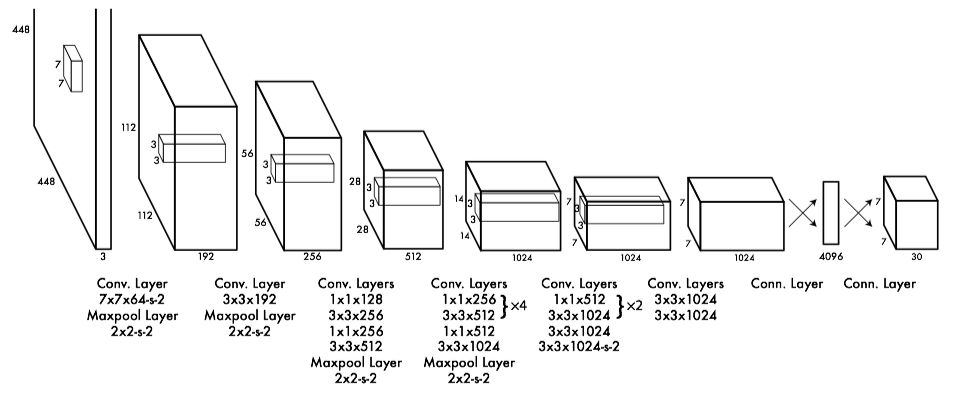
\includegraphics[width=\linewidth]{figures/yolo_v1_network_architecture.png}
    \caption{YOLO v1 network architecture ~\protect\cite{yolov1-paper-2015}.}
    \label{fig:yolo-network}
\end{figure}

\textbf{YOLO v2} \cite{yolov2-paper-2016} is an update of it
previous version to improve the performance while
keeping its speed advantage (67 FPS vs. 5 FPS for Faster R-CNN).
A comparison result with other detector can be found in 
\autoref{fig:yolo-v2-s-acc}. A lot of efforts have been done to make it works:

\begin{itemize}
    \item Added batch normalization layer to gain 2\% improvement in the 
    context of mAP .

    \item Pre-train on ImageNet using images with size $448 \times
    448$ (double from v1) which increases 4\% mAP.

    \item Introduced ``anchor mechanism'' from Faster R-CNN which
    bring 7\% recall improvement.

    \item During training, every 10 epochs change the scale of images to obtain
    more powerful generalization ability.

    \item $13 \times 13$ resolution feature map is enough for ordinary objects
    but in order to overcome the disadvantage from v1 that perform poorly on
    small objects, a passthrough layer has been added that bring the feature
    from an earlier layer at $26 \times 26$ resolution.

    \item Proposed a new backbone network called Darknet-19 which contains 19
    convolutional layers and 5 maxpooling layers.
\end{itemize}

\begin{figure}
    \begin{center}
    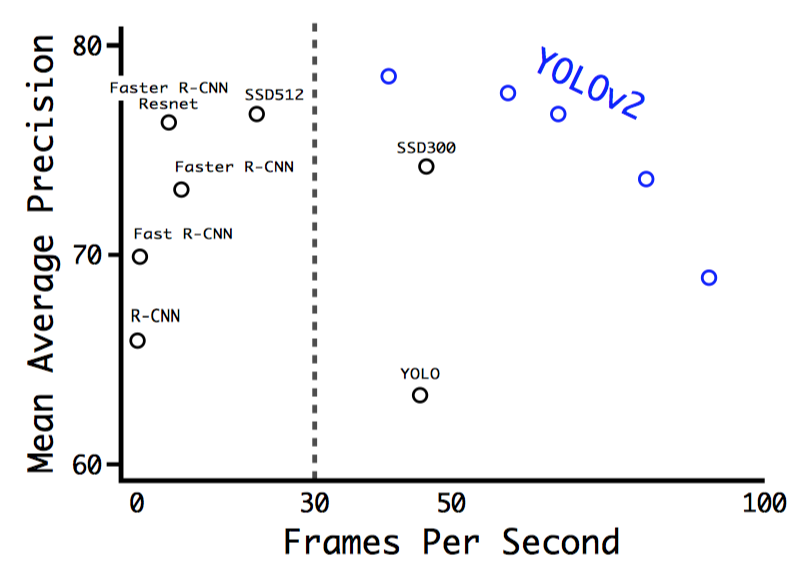
\includegraphics[scale=0.7]{figures/yolov2_speed_and_acc.png}
    \end{center}
    \caption{YOLO v2 accuracy and speed on VOC 2007 dataset
    ~\protect\cite{yolov2-paper-2016}.}
    \label{fig:yolo-v2-s-acc}
\end{figure}

\textbf{YOLO v3} \cite{yolov3-paper-2018}, according to the author, their paper
for this version was not a research paper but technical report. 
It tried a number of tricks and found some of them can push the speed and 
accuracy into a notable line.
A comparison of the inference time between YOLO v3 and most of considerable 
methods can be shown as \autoref{fig:yolo-v3-comp}.

\begin{figure}
    \begin{center}
        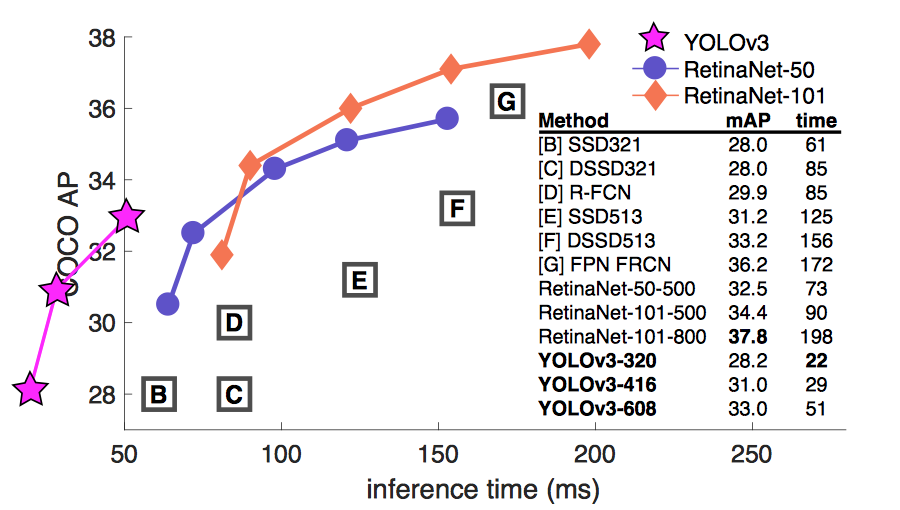
\includegraphics[scale=0.7]{figures/yolov3_comp.png}
    \end{center}
    \caption{Inference time of YOLO v3 compare with others
    ~\protect\cite{focal-loss-for-dense-od}.}
    \label{fig:yolo-v3-comp}
\end{figure}

According to their paper, some significant changes have been applied in this
version:

\begin{itemize}
    \item It designed a new backbone classification network that depended on the
    works of Residual Network \cite{resnet-paper1-2015}
    \cite{resnet-paper2-2016} named Darknet-53 which can improve the top1
    accuracy about 3.1\% while maintaining the speed of 78 FPS.

    \item It discarded the softmax fcuntion for classification instead using a 
    simple logistic classifier. 
    During the training, binary cross-entropy loss was
    employed which can solve the problem of overlapping labels (i.e. man and
    person) in a complex dataset.

    \item It adopted a similar concept of feature pyramid networks (FPN) to
    enhance the scale-invariant ability of the model.
\end{itemize}

\subsubsection{SSD}

Five months after YOLO v1 being published, another famous one-stage approach,
named single shot detector (SSD) \cite{ssd-paper-2015}. 
It achieved much higher performance on mAP metric than YOLO v1, precisely, 
72.1\% mAP on VOC2007 dataset at 58 FPS with $300 \times 300$ input size while 
YOLO v1 only have 63.4 \% at 45 PFS with
$448 \times 448$ input size. The architecture difference between YOLO v1 and 
SSD can be shown by \autoref{fig:ssd_yolo_net}.
To obtain these performances, the following three points contributed a lot:

\begin{itemize}
    \item Employed ``anchor mechanism'' mapping object detection problem to 
    become finding a set of pre-defined bounding boxes.

    \item For each anchor, predicts the class label and the offset of the
    anchor which perform better than regress the absolute location of the 
    bounding box.

	\item For each input, combines feature maps with different scale in order to
    achieve scale invariant.
\end{itemize}

\begin{figure}
    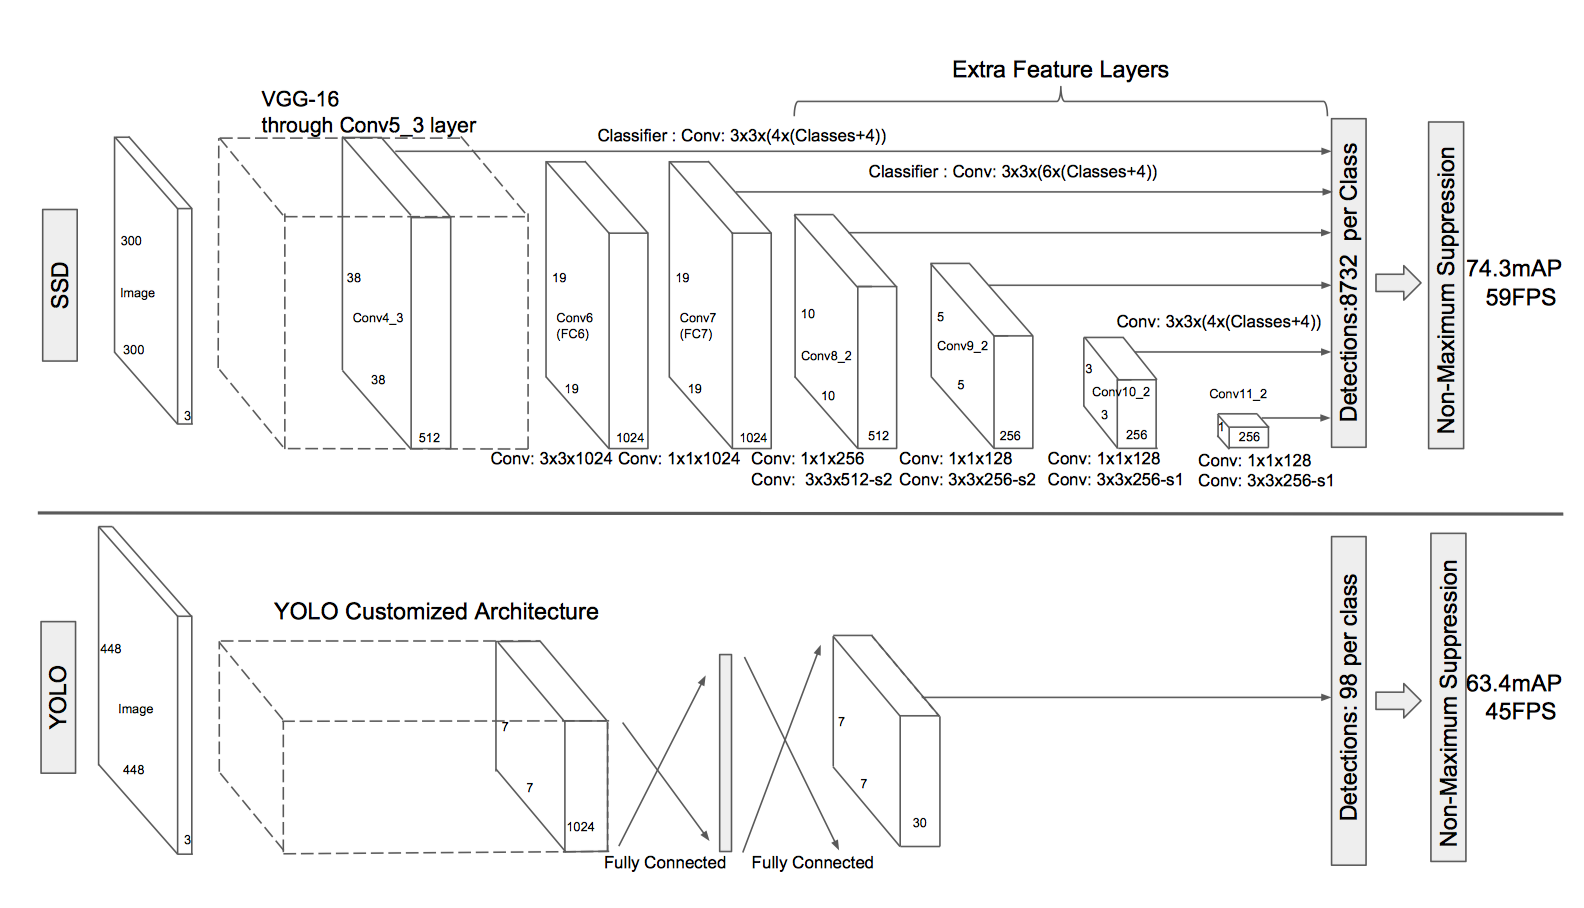
\includegraphics[width=\linewidth]{figures/ssd_yolo_net_arch.png}
    \caption{Network architecture comparison between SSD and YOLO v1
    ~\protect\cite{ssd-paper-2015}.}
    \label{fig:ssd_yolo_net}
\end{figure}

\section{Person Re-Identification}
\label{sec:related_work_re_id}

According to \cite{survey-reid-past-present-feature-2016}, the first definition
of person re-identification was given by Alvin Plantinga in 1961, when he 
discuss the relation between mental state and behavior. It was saying that:

\begin{quotation}
``To re-identify a particular, then, is to identify it as (numerically) the
same particular as one encountered on a previous occasion.''
\end{quotation}

According to \cite{survey-on-dl-for-reid-2019}, let $\delta=\{\delta_1, ...,
\delta_M \}$ represents $M$ descriptors within a gallery set, given a probe
descriptor $U$, the identity of this probe person can be formulated as:

\begin{equation}
\label{general-reid-formula}
I = \arg_{\delta_i} \min (dis(\delta_i, U)),  \: \delta_i \in \delta
\end{equation}

\noindent 
where $I$ represent the identity of $U$ and $dis$ means a proper distance
function which will return the distance between $U$ and all $\delta_i \in 
\delta$. From \autoref{general-reid-formula}, we should notice that there are 
two key points of the person ReID task:
(1) Feature descriptor and (2) Distance function.
How to obtain suitable feature descriptors is always an interesting research
problem in the computer vision area. The traditional way to do it, of course, is
the hand-crafted descriptor which is designed by the experts in this domain, for
example, BRIEF, SIFT, SURF, and ORB descriptors. All these are hand-crafted
descriptors and work well in their own domain. But for distinct tasks, different
descriptors have to be created. Obviously, it requires a lot of work and not
that convenient.

Since 2012, AlexNet \cite{imagenet-classifi-cnn} got a huge success in the
ImageNet classification competition, deep learning boosted. Using deep
neural network as feature extractor becomes popular and its performance defeats
most of the descriptors created manually. In the person ReID community, more 
and more researcher move their attention to the deep learning-based features 
(statistic shown in \autoref{fig:papers-trend}) and a lot of creative methods 
have been developed based on (deep) neural network.

\begin{figure}
    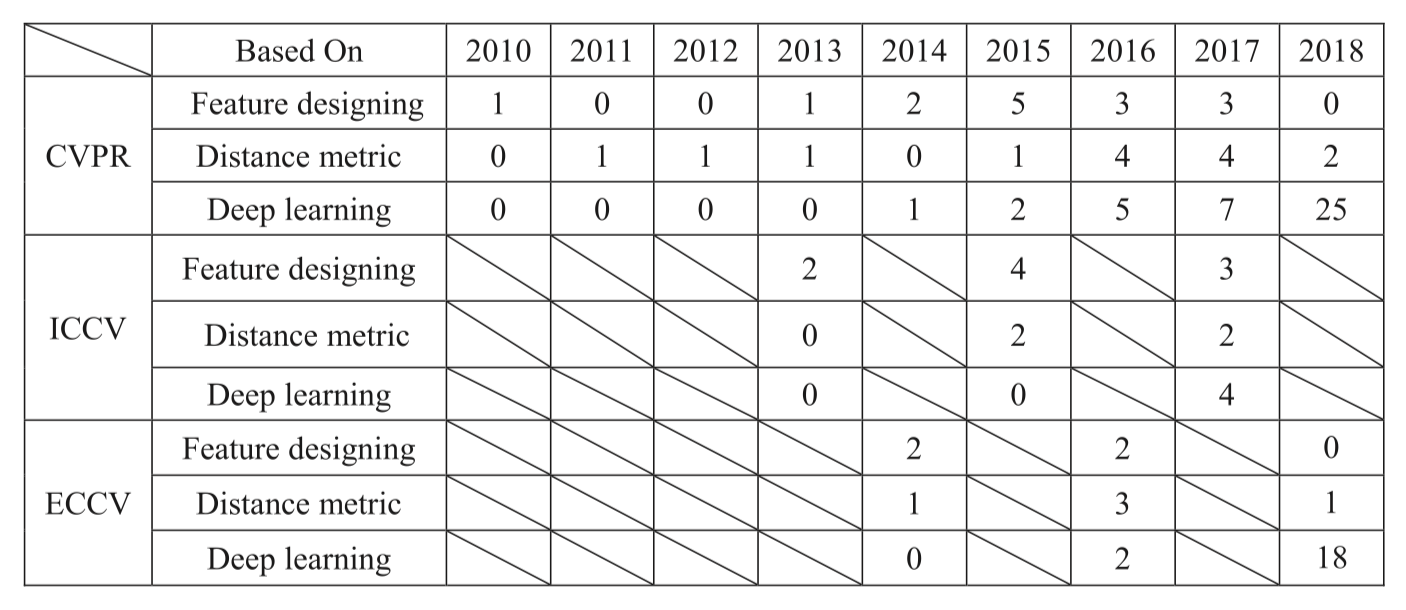
\includegraphics[width=\linewidth]{figures/papers_trend.png}
    \caption{The number of ReID papers depend on different approaches included
    by the three top conferences in recent years
    ~\protect\cite{survey-on-dl-for-reid-2019}.}
    \label{fig:papers-trend}
\end{figure}

In this section, we are going to review the existing deep learning-based 
approaches for the person ReID task, most of them can be sorted into the 
following categories \cite{survey-on-dl-for-reid-2019}:

\begin{itemize}
    \item Identification model
    \item Verification model
    \item Distance metric-based model
    \item Parts-based model
    \item Others
\end{itemize}

We will go deeper into each of these different models in the following
subsections, but mainly concentrate on the identification model and the
distance metric-based model. Because our implementation which will be
introduced in the next chapter is exactly a combination of these two models.

\subsection{Identification Model}
\label{sec:related-work-re-id-idm}

Identification model regards the ReID task as a classification task, distinct
identities will be seen as different classes, the basic architecture of the 
model is shown as \autoref{fig:id-model}. The input to the
network will be the output from some kinds of person detector, then the deep
neural network (e.g. CNN) severs as a feature extractor and by making use of 
these extracted features the input image will be tagged with an identity.

Due to the lacking of data, the main issue of the classification model in deep
learning is always overfitting which means that the model performs pretty good 
on the training set but poor on the validation set. Especially on the person 
ReID task, we want more training samples for each individual but most of the 
dataset only have few sample per instance (e.g. VIPeR only contains two images 
per identity). A lot of works had been done to solve this problem, they can  
roughly be categorized into
(1) add other constraints to revise overfitting and
(2) apply data augmentation techniques or create a larger dataset.

\begin{figure}
    \begin{center}
    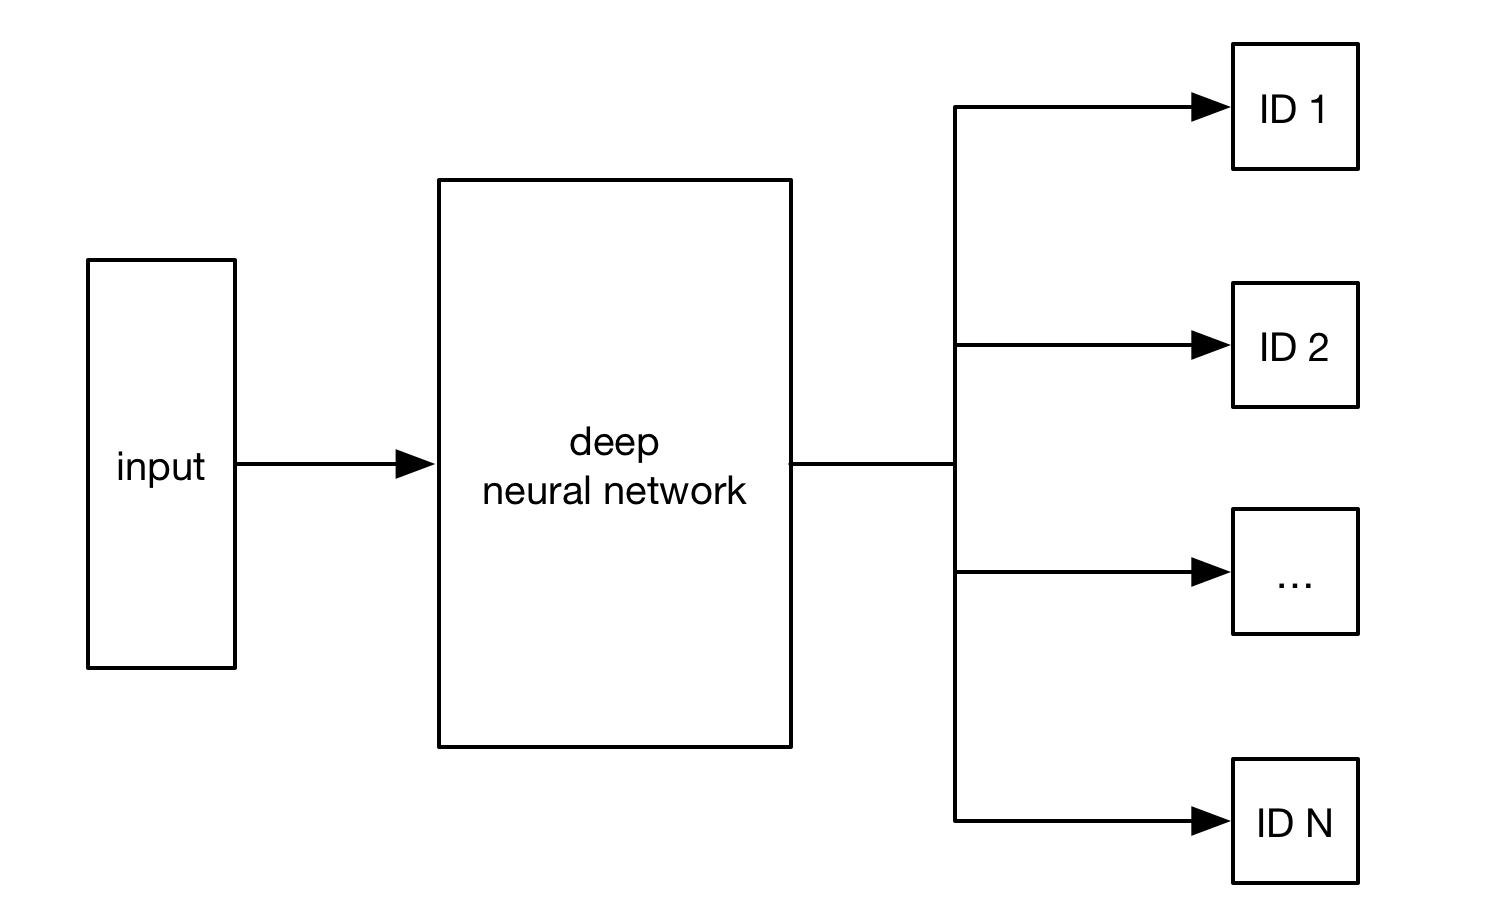
\includegraphics[scale=0.8]{figures/id_model.png}
    \end{center}
    \caption{Architecture of identification model.}
    \label{fig:id-model}
\end{figure}

In \cite{feature-fusion-net-2016}, the authors proposed a fusion feature
network (FFN) which can take both the CNN and the hand-crafted 
features into consideration at the same time, its architecture can be shown as
\autoref{fig:ffn}. FFN takes the identity image as input then branch into two
paths. 
For the CNN feature, five layers convolutional network and two fully 
connected layers were employed. For hand-crafted feature extraction, the 
original image was divided into horizontal stripes then color spaces and 
texture filters were applied in order to extract histograms which finally would 
be concatenated to form a feature vector. 
In the end, theses two kinds of features would be linked together through 
another dense layer. The whole network was trained under the guidance of 
softmax loss function and during back-propagation parameters update would
also be constrained by the hand-crafted feature.

\begin{figure}
    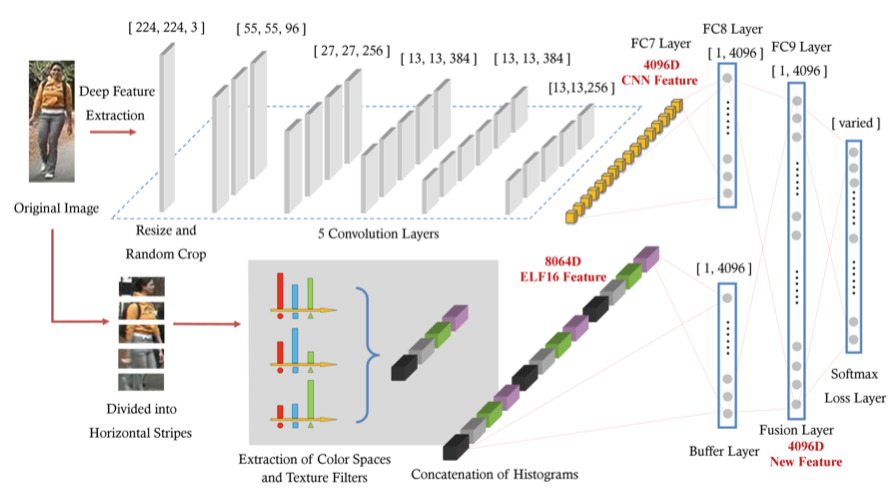
\includegraphics[width=\linewidth]{figures/ffn.png}
    \caption{
        Architecture of fusion feature network 
        ~\protect\cite{feature-fusion-net-2016}.
    }
    \label{fig:ffn}
\end{figure}

The idea behind classification model is that we are trying to use several 
hyperplanes to separate different identities in the feature spaces. But since 
it is a high dimensional space, in some cases, the intra-class variance may 
larger than inter-class variance which is not a good property for a 
classification model.
In order to enhance the learned discriminative feature,
a hybrid network architecture that combined 
with the Fisher vectors which include color histograms and SIFT and a deep 
neural network has been proposed in \cite{hybrid-net-lda-2016}.
%In our implementation, we also target to solve this problem,
%\cite{center-loss-2016}
%which originally proposed for face recognition called ``center loss"
%was employed. It maintains a center point of each identity
%and pushes each image embedding to its corresponding center so the
%variation between the same identity embedding is smaller.

It is worth to mention that when deep learning in person ReID area becomes more 
and more popular, there are several large datasets like
\cite{dataset-cuhk03-2014}, \cite{dataset-market1501-2015}, 
\cite{dataset-dukemtmc-2016} and \cite{dataset-cuhk03-np-2017} have been 
released as well as their corresponding evaluation protocols.
Since deep learning methods really depends on data, these datasets do help the 
community a lot. With the large dataset, we are able to train the 
network directly based on the plain classification model. 
\cite{generic-deep-feature-for-reid-2016} trained the plain classification
network on multiple datasets with domain guided dropout \footnote{Dropout is an 
implemented-friendly but useful technique  to prevent overfitting proposed
by \cite{dropout-paper-2014}.} strategy aiming at 
obtaining a cross-domain model. 

Jointly learning is another hot topic in the deep learning community, it means the model is trained under
the guidance of two or even more loss (objective) functions. In specific person 
ReID research, \cite{comb-id-and-center-loss-2017} proposed a jointly learning 
method which adopted identification loss and center loss 
\cite{center-loss-2016} at the same time, its architecture is shown as
\autoref{fig:comb-center-id-loss}. It claims that it is more efficient than the
pairwise or triplet model and the performance is also better by using their 
feature reweighting layer (FRW). The core idea is that during the training 
time, the model tries to enlarge the inter-class variation
and reduce the intra-class variation supervised by the center loss while
the identification loss makes full use of the image label compared with the 
verification model which just used the weak label information.

\begin{figure}
    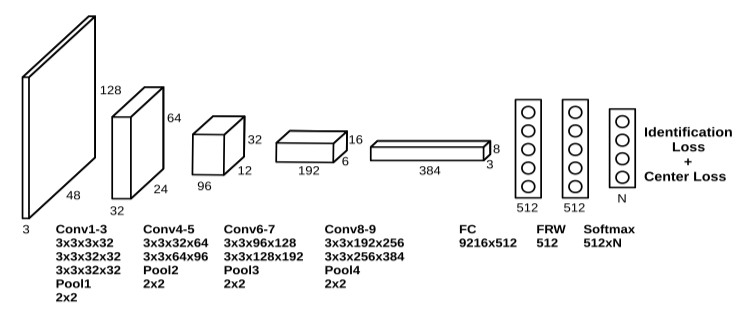
\includegraphics[width=\linewidth]{figures/comb-center-id-loss.png}
    \caption{Architecture of fusion feature network 
        ~\protect\cite{comb-id-and-center-loss-2017}.}
    \label{fig:comb-center-id-loss}
\end{figure}

\subsection{Verification Model}

Verification Model can be seen as a classification problem as well but it is a 
binary version. It takes a pair of images as input and output a similarity 
value indicating whether the paired images is the same person or not. Its 
architecture can be shown as \autoref{fig:vft_model} and simply formulated as:

$$
f(x_1, x_2) =
\begin{cases}
1,&  y_1 = y_2 \\
0,&  y_1 \neq y_2
\end{cases}
$$

\begin{figure}
    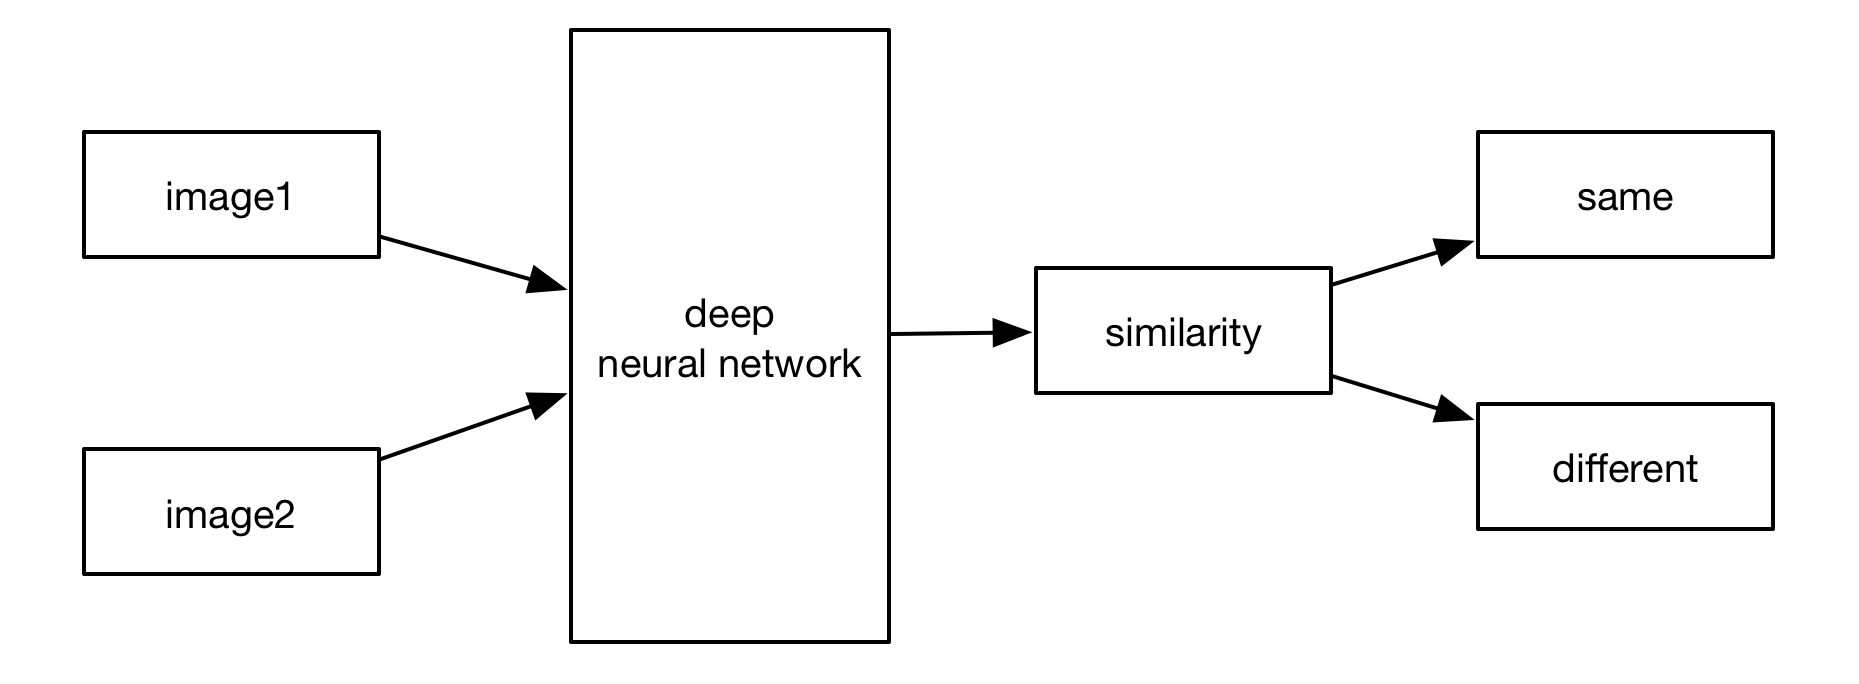
\includegraphics[width=\linewidth]{figures/verification_model.png}
    \caption{Architecture of verification model.}
    \label{fig:vft_model}
\end{figure}

The first verification model to address ReID task named filter pairing
neural network (FPNN) \cite{first-pairwise-net-for-reid-2014} was proposed in 
2014. Max-out pooling layers and patch-matching were employed to jointly handle 
geometric transforms and photometric, misalignment, background clutter and 
occlusions which are common issues in ReID domain.
At the time where datasets were still extremely limited, ``Siamese" deep 
network for metric learning which was firstly
proposed by \cite{first-siamese-net-for-reid-2014} to target this problem. 
Like the common verification model, it takes an image pair as input then pass 
them through three shared parameters but independent convolutional networks to 
perform operations on three non-overlapping parts of the images. The extracted 
feature descriptor will be flattened by a dense layer then used to
compute the cosine distance which would be converted into a similarity value. 
If the value is greater than a hyper-parameter threshold then the input pair 
will be considered as the same identity, otherwise different.
Based on the previous two works, \cite{an-improved-dl-archit-2015} comes up 
with an improved architecture shown as \autoref{fig:cvpr15_model} that include 
a layer to calculate cross-input neighborhood differences which based on 
mid-level features to capture local relationships of the input paired images.

\begin{figure}
    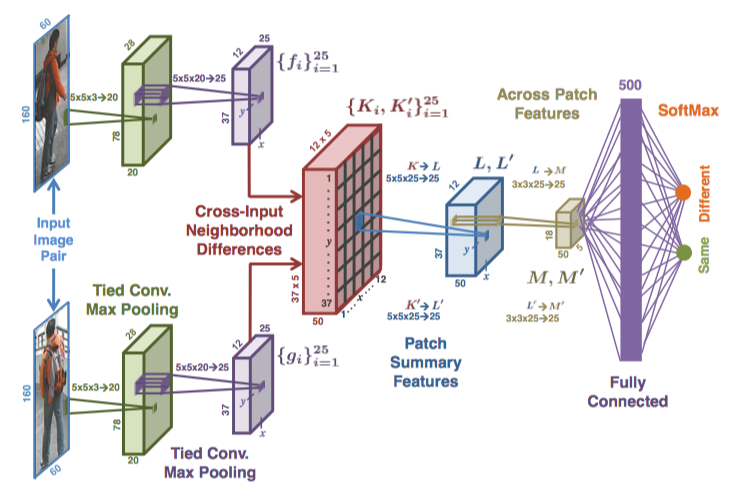
\includegraphics[width=\linewidth]{figures/cvpr15_model.png}
    \caption{Architecture proposed by ~\protect 
        \cite{an-improved-dl-archit-2015}.}
    \label{fig:cvpr15_model}
\end{figure}

But the verification models introduced above all have a common problem which is 
that the neural network employed by them are relatively
shallow. By this limitation, they did not benefit from digging the features 
which are discriminative enough to distinct different identities.
Besides, since we have to construct the image pair for training, there will be 
overhead added compared to the identification model. One more
thing is that the verification models only use the weak dataset label, which 
means that for a specific identity instance pair, it doesn't
care about their actual identity but they are the same or not. Unlike the 
identification model, it will tell directly which identity it is for each
given input.

Because of these limitations, only using the verification model may not achieve 
high accuracy in ReID task. Still, it is worth to mention
that the combination of identification and verification model can reach a 
promising result, \cite{id-verif-combined-learned-cnn-embedding-for-reid-2016} 
proposed such a model and comprehensively compared the advantages and 
disadvantages of these two models. They replaced contrastive loss by 
cross-entropy loss which is different from its sibling network on face 
recognition, then applied dropout regularization to prevent overfitting.

\subsection{Distance Metric-based Model}
\label{sec:related-work-re-id-dism}

The distance metric-based model aims at making the distance between the same 
identity as small as possible while between distinct identity as large as 
possible. One of the most popular used approach is the triplet architecture.
A triplet unit of images can be defined as:
$I_i=\{I_i^1, I_i^2, I_i^3\}$,
where $I_i^1$ called anchor, $(I_i^1, I_i^2)$ is positive pair and $(I_i^1, I_i^3)$ is negative pair.
For each triplet unit, the model will try to satisfy the following:

\begin{equation}
    \label{eq:triplet-model-goal}
    \norm{F(I_i^1) - F(I_i^2)} ^2 < \norm{F(I_i^1) - F(I_i^3)} ^2
\end{equation}

\noindent where $\norm{}^2$ means the L2 norm and $F(I)$ denotes the features 
learned by the model. Based on \autoref{eq:triplet-model-goal}
we can define the loss as following:

\begin{equation}
    \label{eq:common-triplet-loss}
    L(I) = \sum_{i=1}^{n} \max\{ \norm{F(I_i^1) - F(I_i^2)} ^2 - \norm{F(I_i^1) - F(I_i^3)} ^2, C \}
\end{equation}

\noindent where $C$ is a non-negative constant, guided by 
\autoref{eq:common-triplet-loss}, the network will be forced to maximize the 
distance between the anchor-positive and anchor-negative pair under L2 norm, 
the described procedure can be illustrated by \autoref{fig:triplet_objective}.

\begin{figure}
    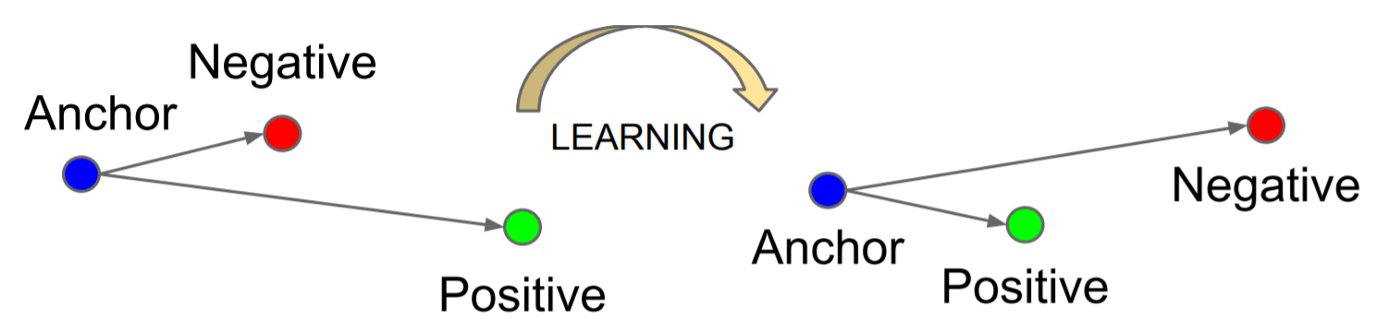
\includegraphics[width=\linewidth]{figures/triplet_objective.png}
    \caption{Objective of triplet loss ~\protect \cite{facenet-triplet-model}.}
    \label{fig:triplet_objective}
\end{figure}

In \cite{in-defense-of-triplet-loss-for-reid-2017}, comprehensive research had 
been conducted to the triplet model, covering the
strategy of sampling, different representations of the loss functions, 
comparison between pre-trained and plain model, etc. Some of their
methods are worth to mention:\\
(1) They proposed a novel way to sample the triplet unit, it says that randomly 
sample $p$ identities within the whole training set and for
each selected identity randomly pick $k$ instances per mini-batch.\\
(2) They came up with several representations of loss functions, the most 
popular two of them are batch-hard loss $L_{BH}$ and batch-all loss $L_{BA}$.
As their name stated, batch-hard loss means to find the hardest triplet units
per batch and use them to contribute to the loss while batch-all loss 
means to use all the triplet units, no matter what they are, contributing 
to the loss. They can be formulated as \autoref{eq:batch-hard}.

\begin{equation}
\label{eq:batch-hard}
     L_{BH} = \sum_{i=1}^{P} \sum_{a=1}^{K}
            [
                m + \max_{p=1...K} D(f_{\theta}(x_{a}^i), f_{\theta}(x_{p}^i))
                - \min_{\substack{j=1...P\\ n=1...K\\ j\neq i}}
                D(f_{\theta}(x_{a}^i), f_{\theta}(x_{n}^j))
            ]_+
\end{equation}

\noindent where $D$ is a distance function, $f_\theta$ is the feature 
descriptor, $m$ is a margin constant, and $[\:]_+$ means the result within 
bracket will be a non-negative number.

\begin{equation}
\label{eq:batch-all}
    L_{BA} = \sum_{i=1}^{P} \sum_{a=1}^{K}  \:
             \sum_{\substack{p=1\\ p\neq q}}^{K} \:
             \sum_{\substack{j=1\\ j \neq i}}^{P} \:
             \sum_{n=1}^{K} \:\:
             [m + d_{j, a, n}^{i, a, p}]_+
\end{equation}

$$d_{j, a, n}^{i, a, p} =  D(f_{\theta}(x_{a}^i), f_{\theta}(x_{p}^i)) - D(f_{\theta}(x_{a}^i), f_{\theta}(x_{n}^j))$$

Effectively, by using $L_{BH}$ we can have $PK$ units contributing to the loss 
while using $L_{BA}$ we have $PK(PK - K)(K - 1)$ units
contribute to the loss. It really depends on the realistic scenario to 
determine which loss we should choose. At this point, it is
significant to note that these two variations of the loss still respect to the 
standard triplet loss function \autoref{eq:common-triplet-loss}.

\noindent 
(3) During the training, they found that using the non-squared Euclidean 
distance is more stable than the squared one which will make the
optimization more prone to collapsing and reduce the interoperability of the 
margin constant (cannot be absolute distance any more).

\subsection{Parts-based Model}

In the very beginning, \cite{hand-crafted-part-based} proposed a hand-crafted
part-based model for matching two persons based on their appearance.
It partitioned a person into horizontal stripes to extract color and texture 
features. After this work, several other researchers \cite{part-based-triangle,
part-based-pictorial-structure} try some more sophisticated strategies to 
divide a person into parts. But still based on hand-designed approaches. 
When deep learning comes to the picture, with the help of from the
research of human pose estimation and landmark detection, the person ReID 
part-based model achieves several impressed results \cite{deep-part-based-glad, 
pose-driven-dcnn-for-reid, pose-invariant-embedding-for-reid}.

Attention mechanism is another milestone in the part-based model, the current 
statue of the art (until this thesis was written) in person ReID task is 
produced by it.
In \cite{end-to-end-attention-network-for-reid}, the author first adopted
attention network to address ReID task, they proposed a LSTM-based
model using a recurrent approach that can output part attention feature 
dynamically for localizing discriminative regions of the pedestrian image. One 
year after, \cite{hpnet-attentive-deep-feature-for-reid} came up with a 
multi-directional attention mechanism for capturing multiple attention
information, the proposed network was named HP-Net.
For the part-based model, there is always a common issue which is the alignment 
problem. Once you divide the image into parts, how to align these chunks and 
calculate the similarity properly will be problematic. To address the 
misalignment issue, \cite{part-aligned-for-reid} introduced a CNN-based 
attention model that makes use of the distance between a paired image to
learn the part-feature for matching. In ECCV2018, \cite{pcb-and-rpp-for-reid} 
proposed a parted-based convolutional baseline model (PCB) which employed a 
simple uniform partition strategy and assembles part-informed feature into a 
descriptor and a refined part pooling (RPP) method which reinforces the 
within-part consistency introducing a large margin of improvement without 
requiring any part labeling information, the architecture shown as 
\autoref{fig:rpp}.

\begin{figure}
    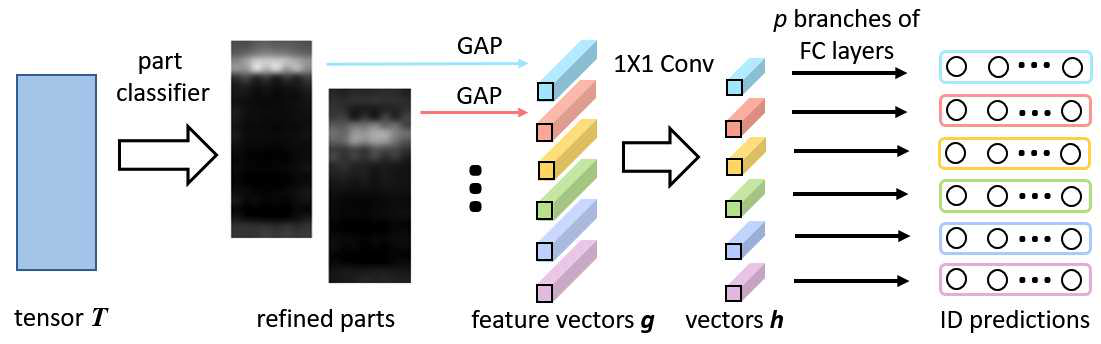
\includegraphics[width=\linewidth]{figures/rpp.png}
    \caption{PCB in combination of refined part pooling ~\protect \cite{pcb-and-rpp-for-reid}.}
    \label{fig:rpp}
\end{figure}

However, the part-based model still has its own limitations:

\begin{itemize}
    \item Adding part-based branches reduced the efficiency of the model.
    \item Most attention-based model only considers region-level attention and 
    discard the pixel-level saliency.
    \item Most of the models do not consider the spatial context information 
    between different part-based features.
\end{itemize}

\subsection{Others}
\label{sec:related_work_other}

Besides the four major models described above, there are still some other deep 
learning-based researches on ReID community.
Even with the datasets like CUHK03, Market1501, and DukeMTMC-reID, the average 
numbers of image per person is still quite limited. The first work try to 
enlarge the dataset with the generative adversarial network (GAN) was 
introduced by \cite{first-gan-for-reid}, they employed GAN to generate 
unlabeled samples and adopt a CNN to extract feature for representation 
learning. Then label smoothing regularization is used for outliers method.

A camera style adaption model to adjust the CNN training was proposed in 
\cite{camera-style-adaptation-for-reid}. 
More precisely, CycleGAN is used to transfer the style of images captured by 
one camera to another. Given an image from camera No.1, the model
can produce the image which looks like captured by camera No.2.

Unlike most of the works which are based on RGB image, it is noteworthy to 
mention a work which employs RGB-D data as input.
A novel method for person ReID using RGB-D data was proposed in 
\cite{rgbd-for-reid}, their working pipeline can be shown as 
\autoref{fig:rgbd-pipeline}.
It took a RGB-D image as input, then performed a segmentation to obtain 
different parts of the human body. By using this information, they
did 3D reconstruction and pose transformation resulting with a standard human 
3D model. Then using the attributes computed from
the 3D model to perform re-identification.

\begin{figure}
    \begin{center}
        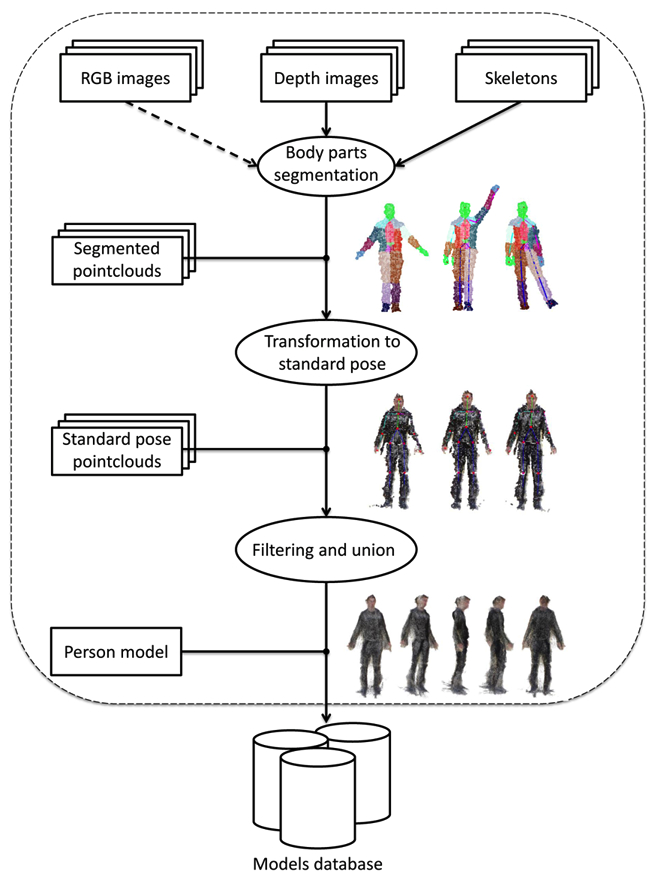
\includegraphics[scale=0.4]{figures/rgbd_for_reid.png}
        \caption{The working pipeline for ReID with RGBD data ~\protect \cite{rgbd-for-reid}.}
        \label{fig:rgbd-pipeline}
    \end{center}
\end{figure}

%\section{OpenISS Framework}
\section{Available Software}
\label{sec:related_work_framework}

To develop a general solution for (1) deep learning-based person 
re-identification and (2) device abstraction, from the implementation point of 
view, we have to survey the currently available software that may be useful for 
our solution.

\subsection{Freenect and Freenect2}
\label{sec:related_work_openiss_freenect}
The most impressive depth camera to people nowadays may still be the Microsoft 
Kinect, even it has been dropped by its own company now. It was the first 
consumptive depth camera in the market released in Nov 2010. Kinect was
designed for Microsoft Xbox 360, a video game console. In order to let the game 
designer to fully make use of it, a corresponding closed source library (known 
as Microsoft Kinect Develop Toolkit) was also released to enable the 
programmability of the device.

Since the Microsoft Kinect Develop Toolkit is closed source and can only be 
used on Windows machines. A group of people from the community makes an 
open-source driver for Kinect named Freenect to enable it works on Linux, MacOS
and Windows. By using this Freenect driver, people can obtain the raw depth 
data from the device directly, a lot of researches based on depth data boost 
increasingly since then. When Microsoft released Kinect v2 (the second version
of Kinect), the community also came up with the driver Freenect2 with the same 
functionality.

\subsection{OpenNI2}

OpenNI or Open Natural Interaction library was originally found by PrimeSense 
which is a depth-sensing solution provider company. Kinect was using their 
technology to obtain the depth data from the sensors. After the
acquisition of PrimeSense by Apple, they shut down the official website but the 
community (like Occipital and other former partners) is still keeping a forked 
version of OpenNI2 active as an open-source library for their product.

By using the OpenNI2 framework, we can perform the following operation using the
same unique APIs, if the hardware driver respect to the OpenNI2 standard.
Fortunately, both Freenect and Freenect2 have the option to build an 
OpenNI2-supported version of them:

\begin{itemize}
    \item Voice and voice command recognition.
    \item Hand gestures.
    \item Body motion tracking.
\end{itemize}

\subsection{OpenCV}

OpenCV is a library of programming functions mainly for computer vision. It
was originally created by Intel (for image processing) in 2000 and now lead by
Itseez. The library is cross-platform and open source under the BSD license,
widely supports most of the existing operating systems. The library was 
originally written in C, but since 2009 it primarily changed to C++. Nowadays, 
it also adds CUDA-based and OpenCL-based GPU calculation, machine learning and
deep learning (TensorFlow, Torch/PyTorch and Caffe) support.

\subsection{NiTE2}
\label{sec:related_work_openiss_nite2}

NiTE2 is a piece of middleware of OpenNI2 library, it has to work with OpenNI2
underneath and provide more powerful functionality than OpenNI2 does. It is
also the design philosophy of OpenNI2 which only supposed to provide the
infrastructure and leave all the other functionalities to the middleware.
Unfortunately, NiTE2 is a closed source library provided by PrimeSense, it was
written in C++ and only comes with the header file and the binary library. By
using NiTE2, we can get the following data:

\begin{itemize}
    \item Skeleton data of the tracked full human body.
    \item Gesture data of the tracked hand.
\end{itemize}

\subsection{RealSense SDK}

RealSense SDK is a cross-platform library from Intel for their own depth
cameras. The SDK allows the developer to access depth and color streaming and
provide the basic camera parameters for calibration. Since the SDK is provided
by the manufacturer directly which means they know everything about the
hardware, it is more powerful than Freenect and Freenect2 as to Kinect. The SDK
is written by C++ and hosted on GitHub, when this thesis is writing, the
community is still quite active and they still try to add more functionalities
to the SDK (like support OpenNI standard, working with OpenCV library, provide
more wrapper for other programming languages rather than C++).

\subsection{CPython}
\label{sec:related_work_cpython}

Our proposed OpenISS framework is designed to be written in C++ since most of
its dependencies list above are in C++. But nowadays, most of the deep learning
programs are written in Python, and for experiment and prototype purposes,
Python has a more efficient development environment. In order to invoke the
deep learning model from OpenISS framework, we need something to connect C++
and Python. CPython is our desired bridge, it is the reference implementation
of the Python programming language written in C and Python. It has a foreign
function interface with support to several other programming languages and C is
one of them. By making use of CPython we can exchange a class, a function, a
variable or other data structure with the languages on two sides of the bridge.

\subsection{TensorFlow}
\label{sec:related_work_openiss_tf}

Since deep learning get boosted recently, there are various of deep learning
frameworks being developed, \autoref{fig:dl-frameworks} shows the popularity of
most of the existing platforms. TensorFlow \cite{tensorflow2015-whitepaper} is
an open-source library written in C++ which designed by Google is one of the
most famous ones. It is a symbolic math library that provides various kinds of
operation to the tensor for dataflow and differentiable programming. It uses
the computational graph with respect to the chain rule to perform
back-propagation which is the core concept for updating the parameters (or we
can say training). Also, TensorFlow can encapsulate the hardware differences and
support training on multiple GPUs if they are available without any code
modification. It becomes more and more popular in the industry and production
environment.

\begin{figure}
    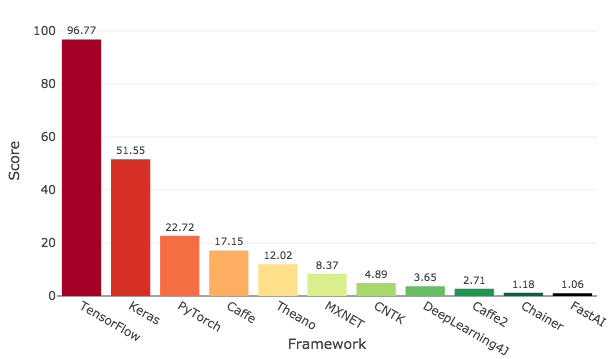
\includegraphics[width=\linewidth]{figures/dl_framework.png}
    \caption{Power score of the most deep learning frameworks in 2018}
    \label{fig:dl-frameworks}
\end{figure}

While TensorFlow is popular in the industry, another framework named Pytorch
gets more attention from academic users like the researchers. In ReID
community, most of the code is based on Pytorch, there is even no baseline
model implemented in TensorFlow and Keras for ReID task.
In contrast, since YOLO is widely used in industry, there are already tons
of existing implementations of YOLO in TensorFlow. In order to keep our
implementation consistent in one framework and reduce the overhead for
translating data from one to another, we choose TensorFlow as our deep
learning platform. By employing it, our research actually fills the gap that no
existing solution for ReID task based on TensorFlow.


\subsection{Keras}

Keras \cite{keras-framework} is a high-level open-source library written in
Python, firstly developed by Francois Chollet, which can take TensorFlow,
Theano and some other frameworks as its back-end. It doesn't provide the
mathematics operation implementation as they were left to the backend but a
human-friendly APIs which can allow you to prototype your conceptual
neural network (or other machine learning architecture) easily and experiment
with different deep learning frameworks. TensorFlow adopted Keras into its core
and announce it as the official high-level APIs in 2017 and more support are
added to Keras since TensorFlow 2.0 which was released in the middle of 2019.

\section{Summary}

In this chapter, we gave intensively review to the most common deep
learning-based methods in both object detection and person re-identification
domains.
%
For object detection problem, we started from the seminal work R-CNN
and stated the key contributions of each existing approach and compare them
with similar methods if comparable. Due to our real-time limitation from the
requirement, we are restricted to use one-stage method. Precisely, we select
YOLO v3 as our detector, because its inference time is large margin better than
all the others and the community already has a lot of existing resources of it.
%
For person re-identification problem, we introduced a total of five different 
models and explain their network architectures and loss functions. Jointly 
considering the trade-off between implementation complexity and the model's 
performance, we decide to use the combination of the identification model and 
triplet model.
%
In the last part of this section, we end up with listing all the available
software that may be employed as dependencies. In the next chapter, we 
will start to present our framework solution.

% EOF

\chapter{Framework Design}
\label{chap:fw-design}
\index{Framework Design}

%%%%%%%%%%%%%%%%%%%%%%%%%%%%%%%%%%%%%%%%%%%%%%%%%%%%%%%%%%%%%%%%%%%%%%%%%%%%%%%%

In this chapter, we are going to describe the design of our proposed solution
which can fulfill the requirements.
We will first explain why we choose the framework solution. Then we outline the 
architecture of our solution. Finally, we detail each component for both the 
core and specialized frameworks.

\section{Why Framework Solution?}
\label{sec:fw-design-why}

In the context of software engineering and computer programming, a software
framework is an abstraction in which software providing generic functionality
can be selectively changed by additional user-written code, thus providing
application-specific software \cite{wikipedia-software-framework}.
According to \cite{software-framework-def}, a software framework consists of
two components:

\begin{itemize}
    \item Frozen spot, within a framework, defines the overall
    architecture of a software system, that it is to say its basic components
    and the relationships between them. These remain unchanged in any
    instantiation of the specialized framework.

    \item Hot spot, within a framework, it represents those parts where the
    programmers using the framework write their own code to add specific
    functionalities based on their own need.
\end{itemize}

There are three key distinguishing features the make a framework different from
the normal software libraries:

\noindent \textbf{Inversion of control:}
In a framework, the program's flow of control, unlike in libraries or
applications, is not dictated by the caller but the framework.
%
In our case, since we want to address the person ReID problem (specified by
\textbf{FR4} and \textbf{FR5}) which can be
divided into two subproblems: person detection and person retrieval.
The output from the former will be the input of the latter, from the user's
point of view they are totally not interested in the intermediate result but
want the final result directly. So the user doesn't have the knowledge and they even
don't want to know how the data flow between these two subproblems and how the
the device can obtain the raw data as well.
The flow of control should actually be done by the framework since for a
specific task, the workflow should be deterministic and the user just tells what
they want to do but not how they do it. Under such consideration, having
the program's flow predictable and controllable is extremely important for us.

\noindent \textbf{Non-modifiable framework code:}
The framework code (aka. frozen spot), in general, is not supposed to be
modified, while accepting user-implemented extension (hot spot). In other
words, users can extend the framework, but cannot change its code.
%
The reason why the frozen spot cannot be changed is that the framework is
responsible for controlling the flow of the program, without knowing what
kind of application the framework will be used for. The control flow is defined
by these frozen spots, if they are always changed then there is no way to
achieve inversion of control.

\noindent \textbf{Extensibility:}
A user can extend the framework, usually by selective overriding or add
specialized code to provide specific functionality.
%
As mentioned in \autoref{sec:intro-non-func-req}, extensibility is one of our
non-functional requirement. Since we want to support various kind of cameras
(specified by \textbf{FR1} and \textbf{FR2})
and as introduced in \autoref{chap:RelatedWork} the algorithms for both person
detection and person retrieval are diverse. It is possible that later on we may
want to perform comparisons among these algorithms. With such design in advanced,
we can save a lot of jobs for integration and it also makes our solution more
valuable.

From the discussion above, we see that the key features of a software framework can
perfectly fit to the demand of our solution. If we think in an abstract way,
what our solution needs actually is to enable the definition of a pipeline.
Every pipeline has the same structure:
\begin{enumerate}
    \item Information is gathered by devices which can be diverse;

    \item Information is transformed/extracted using filters, which can also be
          diverse but must be made abstract so that they can easily
          interoperate;

    \item Every device and filtering algorithm comes with their own data model;
\end{enumerate}

Interoperability comes through the definition of an abstract data
structure that is exchanged between the abstractly defined filters. This way,
various devices can be used in conjunction with various filtering algorithms to
create an application. This is, in fact, a classic example of a problem solvable
using a framework approach. So we decide to plan our solution in a framework
manner.
In our design, we have the core framework as the frozen spot which
defines the infrastructure like device, cross-language calling mechanism and
viewer.
Then for each specific purpose, we have a specialized framework which under the
core framework umbrella providing specific functionalities for various
application developers like person ReID, skeleton tracking, gesture tracking
and facial expression recognition.

\section{Core Framework Design}
\label{sec:fw-design-core}

In a very high-level description, we design our framework OpenISS consisting of
total eight components shown as \autoref{fig:fw-core-module}. Each box in
green represents a frozen spot of the core framework and each box in yellow
means a set of frozen spots which can combine with the core to form a
specialized framework.

For the five core frozen spots, their functionalities are designed as follows:

\begin{itemize}
    \item Device module: it provides an abstraction of various devices which
    can be used by any application that needs depth cameras as input.

    \item Cross-language module: it provides the ability that from C++ we can
    invoke algorithms or models implemented in Python which can help us to make
    sure of most of the existing resources available from the community.

    \item Pipeline module: it serves as an executor of the framework providing
    the flow of control for a variety of tasks.

    \item Common data structures: it provides our own framework data structures
    which were adapted from other low-level libraries or software enabling us
    to perform our own algorithm independently.

    \item Viewer module: it provides visualization abstraction of the framework
    can be used by any application that needs to show the result visualized
    (e.g. display result image).
\end{itemize}

For the three specialized frameworks, they are designed to:

\begin{itemize}
    \item Tracker specialized frameworks: it provides the abstraction of a tracker,
    in the context of motion capture, computer vision or image processing,
    which takes a frame from a sequence of images and a set of given pixels as
    input. Then for all the remaining frames in the sequence keep tracking
    location of the same set of pixels that have the same meaning.

    \item Detector specialized frameworks: it provides the abstraction of a
    detector, in the context of computer vision, which takes an image and an
    object class list (e.g. cat, dog, person, car) as input then output a
    bounding box for each detected object instance within the given list.

    \item Recognizer specialized frameworks: it provides the abstraction of a
    recognizer, in the context of computer vision, which takes an image (can be
    a pedestrian or a face image) or video (a video with facial expression or
    gesture) as input then output whether this image or video have been seen
    before (within the pre-defined database or by any other means).
\end{itemize}

\begin{figure}
    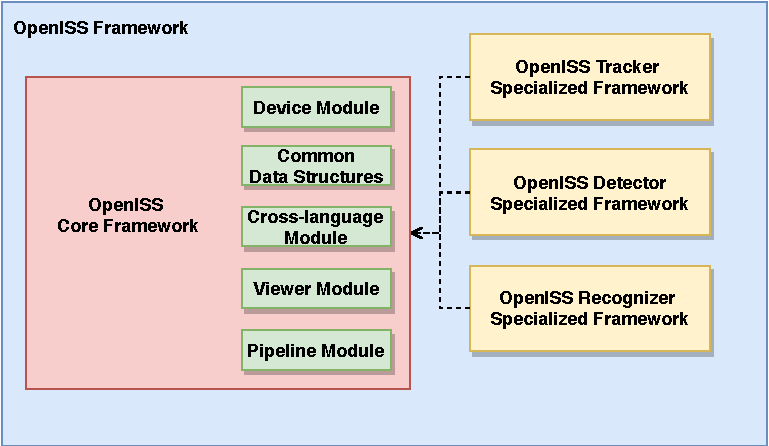
\includegraphics[width=\linewidth]{figures/framework_core_module.pdf}
    \caption[Core components of OpenISS framework]
    {Core components of OpenISS framework, each box in green means the core
    framework's frozen spot and each box in yellow represents a set of frozen
    spot of each specialized framework.}
    \label{fig:fw-core-module}
\end{figure}

In the following paragraphs, we are going to explain the design of the core part of
each module within the core framework.

\subsection{Device Module}
\label{sec:fw-design-core-device}

Device module is one of the most essential modules in the whole OpenISS
framework because it is the lowest layer from our framework's point of view. It
is designed directly on top of the hardware drivers from various device
manufacturers.
Our design goal for this module is that we would like to block the physical
differences of cameras accessing them via a set of common APIs. Also, the
design should allow us to add support to more kinds of cameras easily without
changing the frozen spots itself.

With those requirements in mind, we found that one possible solution is to make
use of the polymorphism feature and dynamic dispatch mechanism, accessing the
subclass's method via a reference of its superclass. So what we need to do
will be just to come up with an elaborate abstraction that can be applied to
most of the common devices. After overall consideration, our design for the device
module shown as \autoref{fig:fw-core-device}. Since it is a core module, we are
going to explain some of these important abstract methods defined
in \texttt{OIDevice} class:

\begin{itemize}
    \item \texttt{rawDevice}: Sine our device model need to depend on
    the hardware driver, sometimes we may want to access the original device
    object created by the driver, this method is designed for it.

    \item \texttt{init}: This should contain the logic used to initialize
    the device, usually we need to call the driver's \texttt{init} method.

    \item \texttt{open}: This method is used for opening the device, it
    should be called after \texttt{init} method.

    \item \texttt{close}: This method is used for closing the device
    logically, most of the time we will release the resources which are not
    needed anymore.

    \item \texttt{enable}: This method is a shortcut for the following
    three specific enable methods.

    \item \texttt{enableColor}: This method tells the device to enable
    the color data stream.

    \item \texttt{enableDepth}: This method tells the device to enable
    the depth data stream.

    \item \texttt{enableRegistered}: This method tells the device to
    enable the registered data (infrared image data, aka. IR data) stream.

    \item \texttt{getIntrinsic} and \texttt{getExtrinsic}:
    These two methods are designed to obtain the intrinsic or extrinsic matrix
    respectively of the device if they are provided by the hardware driver.

    \item \texttt{getDepthScale}: This method is used to get the depth
    scale value which multiplies the depth data value can get the distance of
    in meter or centimeter.

    \item \texttt{readFrame(StreamType type)}: This method is the
    most important one, it is used to get a frame of data respect to the stream
    type (color, depth or IR) specified by the parameter.
\end{itemize}

\begin{figure}
    \centering
    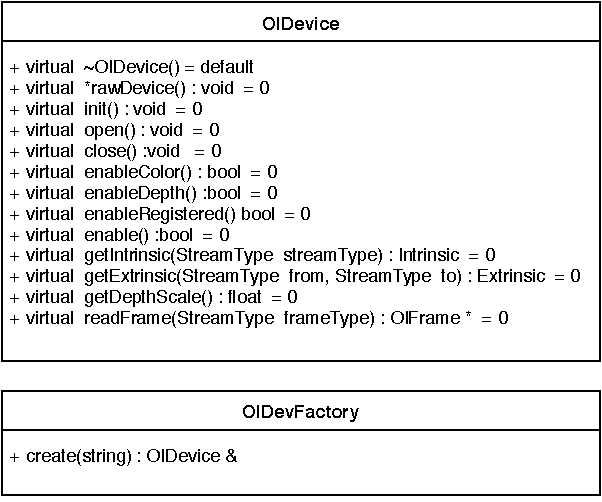
\includegraphics[scale=0.8]{figures/framework_core_device.pdf}
    \caption{Design of device module within OpenISS core framework.}
    \label{fig:fw-core-device}
\end{figure}

\subsection{Cross-Language Module}
\label{sec:fw-design-core-cross-lang}

As mentioned in \autoref{sec:related_work_obj_det} and
\autoref{sec:related_work_re_id}, since 2012, deep learning approach dominates the
research community of both object detection and person re-identification.
Nowadays most of the available deep learning frameworks provide Python APIs for
convenient purpose, even though themselves were written in C/C++, developing
deep learning program directly using low-level APIs makes the works tedious and
problematic.
In order to address this issue, we design the cross-language module shown as
\autoref{fig:fw-core-cross-lang} which
enable the user to separate deep learning oriented program development from the
normal programming task. Our OpenISS framework itself is written in C/C++ (the
reason will be explained later in \autoref{sec:fw-inst-impl}), but for the deep
learning-based
models, we decide to develop them in Python then provide an encapsulated
internal API to invoke Python model from C/C++ by employing CPython introduced
in \autoref{sec:related_work_cpython}. It can not only help us to decouple the
framework's functionalities but also make good use of the existing community
resources.

\begin{figure}
    \centering
    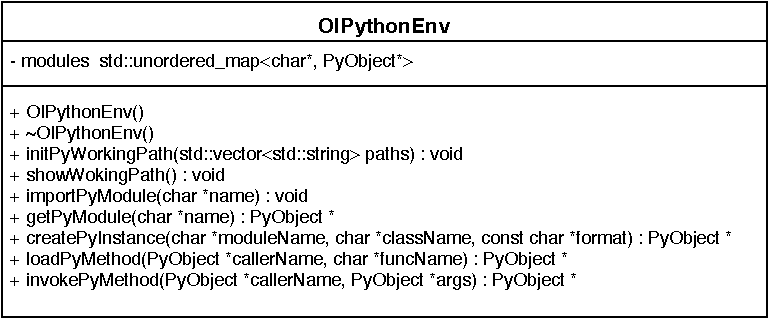
\includegraphics[scale=0.8]{figures/framework_core_cross_lang.pdf}
    \caption{Design of cross-language module within OpenISS core framework.}
    \label{fig:fw-core-cross-lang}
\end{figure}

The \texttt{OIPyhonEnv} is not an abstract class,
%class but a concrete one so
%that by definition it cannot be counted as frozen spot of the framework.
the reason why we put it under the core framework is that it actually serves as
an infrastructure even though the classes which will invoke the Python code
don't need to inherit from it but they have to use it as a dependency.
The \texttt{OIPythonEnv} class is used to encapsulate a Python script, four
core functions \texttt{initPyWorkingPath}, \texttt{createPyInstance},
\texttt{loadPyMethod} and \texttt{invokePythonMethod} are respectively used to
add a given path to the Python interpreter as a working path (Python will search
the requested module under all the working paths), create an object of a given
class which is visible within the encapsulated Python script, load (without
execute) the handler of a specified method which is visible from that file and
invoke a loaded function using its handler.

The design and usage philosophy of this module illustrated by
\autoref{fig:fw-core-cross-lang2} is that each instance of \texttt{OIPythonEnv}
can be used for representing a Python file (the box in green), a framework
developer trained, in our case, a deep learning model in Python (the red box)
and would like to expose some of the functionalities of it to the framework
users. Then they can write a C/C++ wrapper (the blue box) for it which
contains a member variable of type \texttt{OIPythonEnv} instantiating with the
names of classes and functions would like to expose. The framework users then
can use the Python code via our framework without knowing anything about Python
under the hood.

\begin{figure}
    \centering
    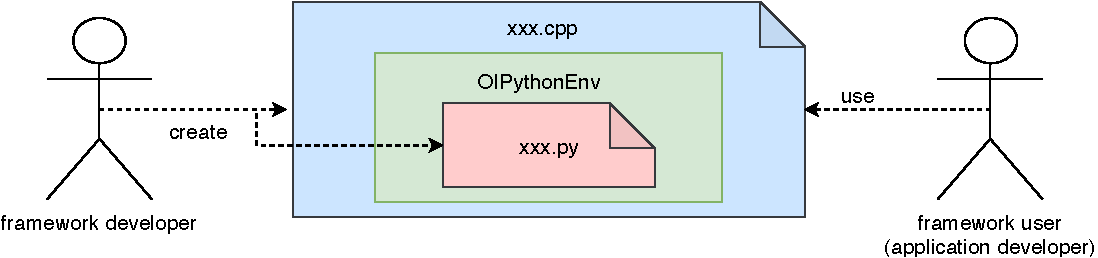
\includegraphics[scale=0.8]{figures/framework_core_cross_lang2.pdf}
    \caption
    {Usage scenario of the cross-language module of OpenISS core framework.}
    \label{fig:fw-core-cross-lang2}
\end{figure}

\subsection{Pipeline Module}
\label{sec:fw-design-core-pipeline}

\begin{figure}
    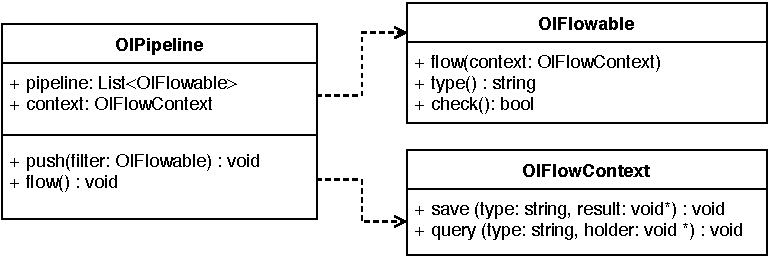
\includegraphics[width=\linewidth]{figures/framework_core_pipeline.pdf}
    \caption{The design of the pipeline module in the core framework.}
    \label{fig:fw-core-pipeline-uml}
\end{figure}

The pipeline module, as its name implies, provides a pipeline execution
mechanism to the framework users. It allows the user to chain multiple
components together that the former's output will become the latter's input.
When all these filters finish execution, we can achieve some specific goal, for
example, our final goal, tracking person across multiple cameras (detail will
be explained in \autoref{chap:fw-app}).

The design of the module can be described by the UML diagram shown as
\autoref{fig:fw-core-pipeline-uml}. The \texttt{OIPipeline} class contains a
list of filters and a reference with type \texttt{OIFlowContext} which is an
abstract class used to define the save and query behaviors of the temporary
result generated from the intermediate filter. The \texttt{push} method is used
to add a concrete filter into the pipeline while the \texttt{flow} method is the
switch to trigger the pipeline execution process.
The component which would like to serve as a filter must implement the
\texttt{OIFlowable} contract. There are three functions defined within this
interface:

\begin{itemize}
    \item \texttt{flow}: it takes a reference of \texttt{OIFlowContext} as
    parameter, basically what this function does is calling the real logic
    method. For example, the \texttt{flow} function will call the
    \texttt{readFrame} function within \texttt{OIDevice}, the \texttt{detect}
    function within \texttt{OIDetector} and the \texttt{predict} function
    within \texttt{OIRecognizer}.

    \item \texttt{type}: it just returns the type of the filter itself, we may
    need it to differentiate some operations for various filters.

    \item \texttt{check}: it usually gets called before \texttt{flow} method,
    we perform necessary checking step here to ensure all the needed data are
    available before \texttt{flow} get executed.
\end{itemize}

The control flow of the pipeline module can be expressed by
\autoref{algo:fw-pipeline-flow} and the workflow can be visualized by
\autoref{fig:fw-core-pipeline}. With the \texttt{OIPipeline} class
definition in mind, there are two fields: \texttt{pipeline} which is a list of
filters and \texttt{context} which is actually a temporary data holder.
What we eventually do is that we loop over all the filters within the list and
invoke their \texttt{flow} method which is implemented in the concrete
classes and store the result in the concrete implementation of the
\texttt{OIFlowContext} class.
Inside the abstract \texttt{OIFlowContext} class, we define two methods:
\texttt{query(name:string, data:void*)} and \texttt{save(name:string,
data:void*)}. The method \texttt{query} is used to lookup the needed input
which output by the preceding for current executing filter while the
\texttt{save} function is used to save the temporary result generated by
the current filter. If there is more than one input or output from the current state,
we just need to call these two functions multiple times so we don't limit
ourselves to the number of input and output of a filter.

\begin{algorithm}
    \ForEach{filter in pipeline}{
        canFlow = filter.check(context)\;
        \If{canFlow}{
            result = filter.flow(context)\;
            context.save(filter.type(), result)\;
        }
    }
    \caption{The \texttt{flow} function within \texttt{OIPipeline} class}
    \label{algo:fw-pipeline-flow}
\end{algorithm}

\begin{figure}
    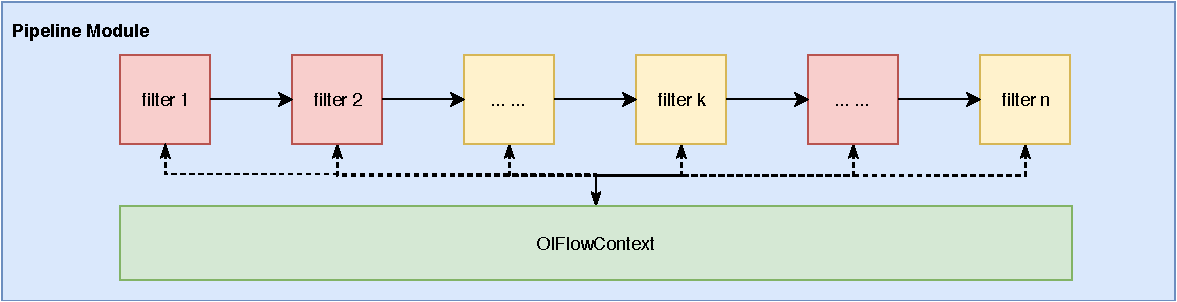
\includegraphics[width=\linewidth]{figures/framework_core_pipeline2.pdf}
    \caption{The design of the pipeline module in the core framework.}
    \label{fig:fw-core-pipeline}
\end{figure}

As you may notice the \texttt{OIPipeline} class, only have the method
\texttt{push} to allow the user to add filters but it doesn't provide any
removal interface for the existing filters which means each \texttt{OIPipeline}
instance is immutable. In other words, once it being defined you cannot change
its internal structure.
We design in such a way under the consideration that each pipeline instance is
used for a specific task. If you have more than one task then you will need to
reassemble a new pipeline instance and create another concrete
\texttt{OIFlowContext} object but you can reuse the same filter object if you
want. Also, all the filters reside in the pipeline are chained linearly. But
when you executing them, a conditional operation can be achieved by the
\texttt{check} method since it is the predecessor of the \texttt{flow} method.

\subsection{Common Data Structures}
\label{sec:fw-design-core-common-ds}

Common data structures, in OpenISS core framework, means these data structures
may be used by other modules within the core or cross multiple specialized
frameworks.
\texttt{OIFrame} is one of the most significant data structure of our
framework which is designed to represent the data captured by an input device
at a certain point of time. It will flow between the core and
specialized framework or even between several different specialized frameworks.
The design of \texttt{OIFrame} can be illustrated as
\autoref{fig:fw-core-oiframe}, the \texttt{OIFrame} is the highest level
abstraction provides the fundamental information of a frame. It has two
subclasses named \texttt{OIAbstractDataFrame} and \texttt{ICvImplFrame}, the
former is still an abstract class representing a frame contains data and the
latter is a concrete class describing a frame provided to the viewer.

\begin{figure}
    \centering
    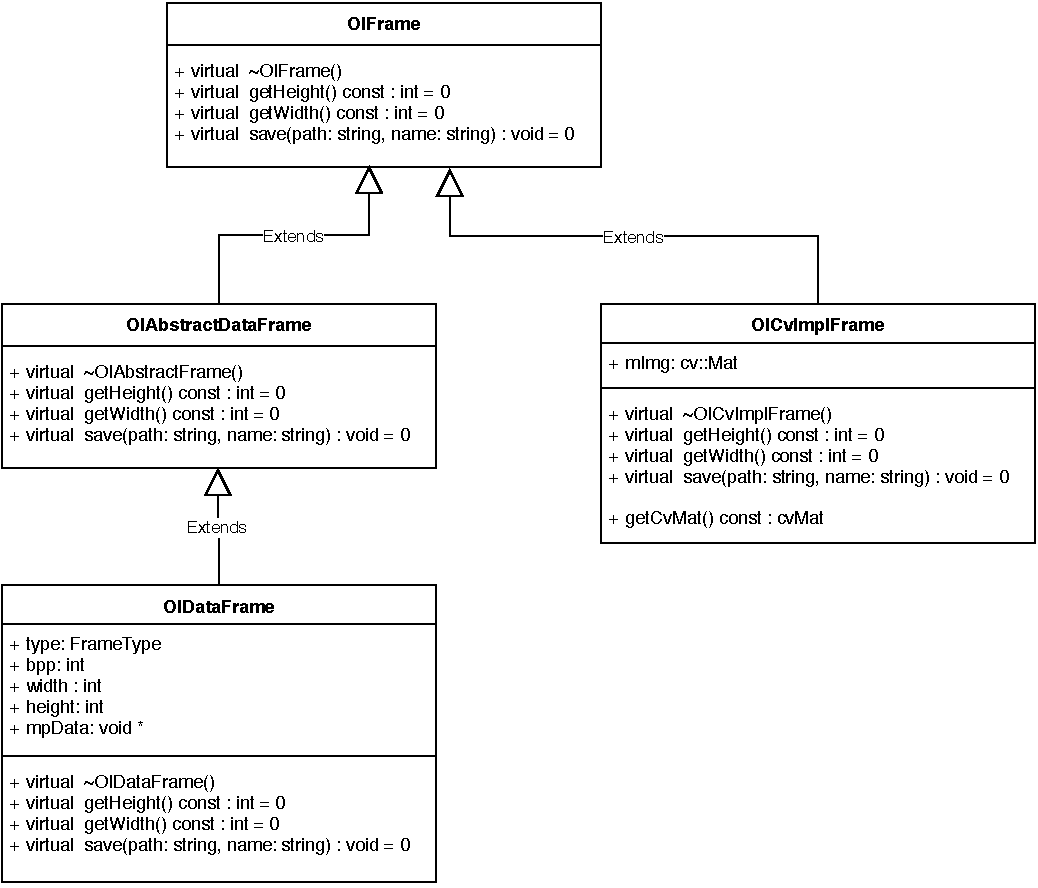
\includegraphics[width=\linewidth]{figures/framework_core_oiframe.pdf}
    \caption{
        Design of \texttt{OIFrame} inside common data structure within the core
        of OpenISS framework.
    }
    \label{fig:fw-core-oiframe}
\end{figure}

\subsection{Viewer Module}
\label{sec:fw-design-core-viewer}

The responsibility of the viewer module is straight forward and simple, as its name
implies, it is used for displaying the data for visualization purposes. Our
design for the viewer module is simple, as shown in
\autoref{fig:fw-core-viewer}, \texttt{OIViewer} is an abstract class which
contains a variable and a method. The variable \texttt{name} is an label used
to differentiate from various of displaying windows since the user may want to
show more than one frame, for example, show both color and depth image a the
same time.
The method \texttt{show} contains the logic for various libraries for
drawing. Currently, our framework only has one concrete implementation which
is \texttt{OIOpenCVViewer} based on the OpenCV library.
The \texttt{OIOpenGLViewer} implementation was designed but is still under
development.

\begin{figure}
    \centering
    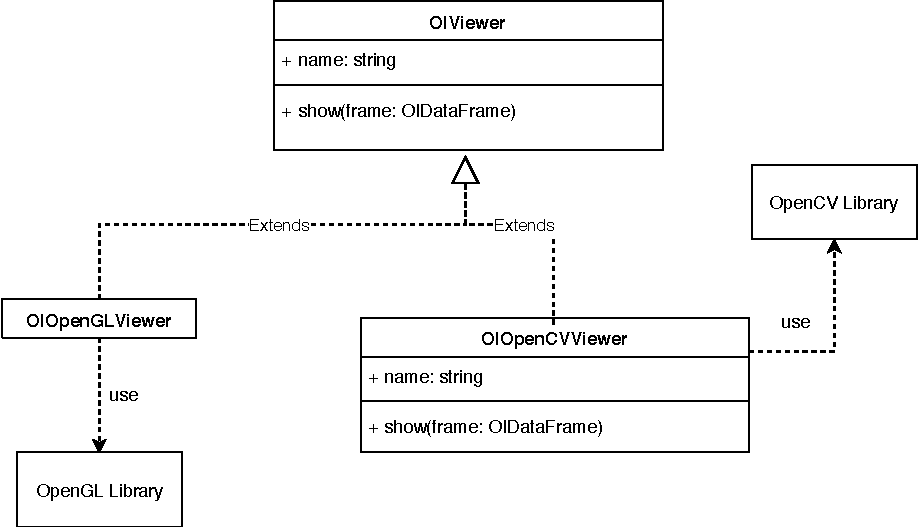
\includegraphics[scale=0.8]{figures/framework_core_viewer.pdf}
    \caption{Design of viewer module within the core of OpenISS framework.}
    \label{fig:fw-core-viewer}
\end{figure}

\section{Specialized Framework Design}
\label{sec:fw-design-spec}

The specialized framework is designed for solving a class of specific problems,
it provides a set of unified APIs to the framework users just like other
modules within the core framework but also defines the problem-specific data
structures and common methods. In an abstraction description, the data flow
within the framework can be viewed as \autoref{fig:fw-design-dataflow}. The raw
data from the physical device will firstly flow into the core of the framework
handling at least by the device module. Then these raw data will be wrapped to
become our OpenISS data structures and keep flowing into one or a pipeline of
specialized frameworks, since normally a large problem can be divided into
several subproblems, we believe that the combination of these specialized
frameworks may be able to solve more complex problems so we decide to make the
specialized framework chainable. Finally, the data will be converted into the
user's expected format and reach the end-user's application.

\begin{figure}
    \centering
    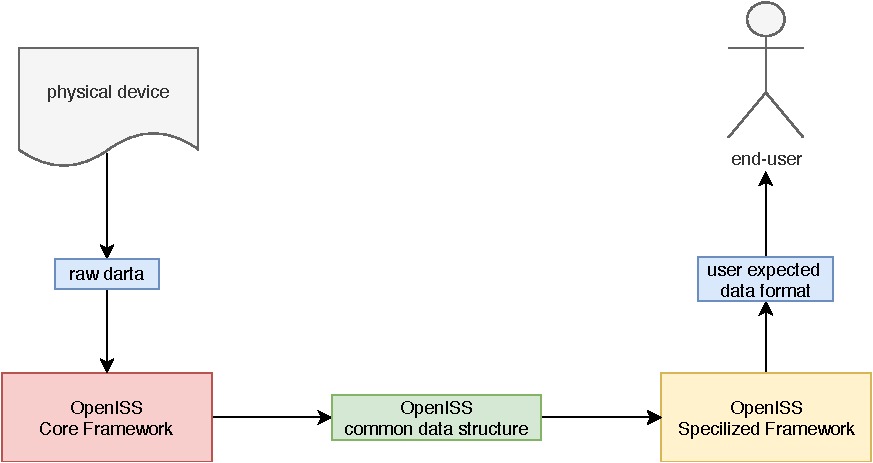
\includegraphics[scale=0.8]{figures/framework_dataflow.pdf}
    \caption{Data flow within the OpenISS framework.}
    \label{fig:fw-design-dataflow}
\end{figure}

In this thesis, we proposed three specialized frameworks, shown as the
rectangle in yellow in \autoref{fig:fw-core-module}. A combination of two
of them (detector and recognizer) aiming re-identify the same person across
multiple cameras in order to solve the limitation we mentioned in
\autoref{sec:intro-lim-issv2}.
And the other one (tracker) is used for skeleton tracking.
In this section, we will describe the architecture of each specialized
framework.
%and explain how the detector and recognizer can work together to
%achieve person ReID task.

\subsection{Tracker Specialized Framework Design}
\label{sec:fw-design-spec-tracker}

In \autoref{sec:intro-scen-req}, we explained the need for skeleton tracking.
Also, at the same time when this thesis is writing, there is another work
happening which aims at providing the functionality of gesture tracking. So it
is necessary for us to abstract the common methods of skeleton tracker, gesture
tracker and all other possible trackers.
Recall the problem a tracker attempt to address is that for a given sequence of
frames and a target, it is expected to locate the target for each of the
remaining frames.

In order to achieve that we design the tracker specialized framework shown as
\autoref{fig:fw-sub-tracker}. \texttt{OITrackerFactory} is responsible for
instantiating the concrete tracker object and tracker frame object.
\texttt{OITracker} is the abstract class of the tracker, it defines three basic
methods, \texttt{startTracking} for starting tracking, \texttt{stopTracking}
for stopping tracking and \texttt{readFrame} for reading data from the input
source and apply tracking algorithm on it that is where the magic should be
implemented in its subclass. The parameter, \texttt{OITrackerFrame}, acts as a
data container, the result of the tracking will be placed within this class and
it will be updated per frame time.

\begin{figure}
    \centering
    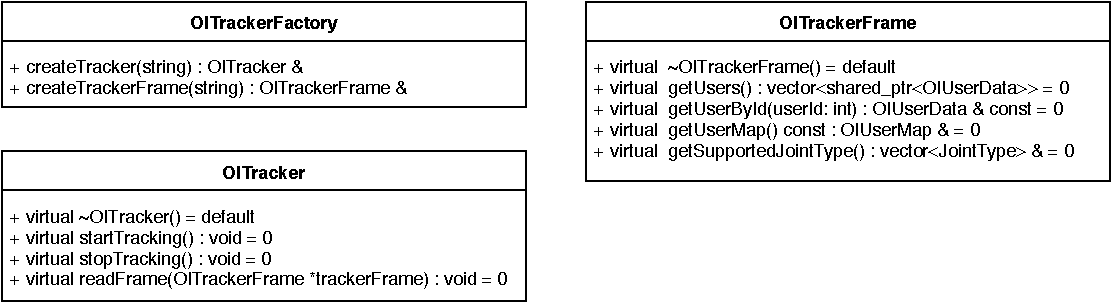
\includegraphics[width=\linewidth]{figures/framework_sub_tracker.pdf}
    \caption{Design of the OpenISS tracker specialized framework.}
    \label{fig:fw-sub-tracker}
\end{figure}

\subsection{Detector Specialized Framework Design}
\label{sec:fw-design-spec-detector}

As mentioned in \autoref{sec:intro-pbstat}, our research problem can be divided
into two parts and one of them is object detection, more precisely, pedestrian
detection. So it is necessary to design a specialized framework for it. Since
we are designing a framework, in order to maintain its abstractness and
extensibility, we need to extract the common parts of different kinds of
detector and provide an abstraction of them.
Recap the definition of object detection we gave in \autoref{sec:intro-pbstat},
given an image $I$ and a list of objects $C$, the output will be a list of
bounding box $B$ which contains the instances of objects listed in $C$.

With such consideration, we design the specialized framework as
\autoref{fig:fw-sub-detector} shown. The \texttt{OIDetector} is the abstract
class which will be exposed to the user. Depends on the user's specific demand,
they can use either our pre-defined hot spot or create their own hot spot to
perform different kinds of detection algorithm. The frozen spot itself
\texttt{OIDetector} has a member variable \texttt{classList} contains the name
of the supported classes of a detector and a method named \texttt{detect} which
take an instance (hot spot) of the OpenISS common data structure
\texttt{OIFrame} as input and output a list of bounding boxes with the type
\texttt{OIBBox}.
Since the detector may be used to detect any kind of objects the shape of the
bounding box may be different. \texttt{OIBBox} is the abstract class of the
result which currently has two pre-defined hot spots \texttt{OIBBoxRect} and
\texttt{OIBBoxCircular} representing the rectangular and circular shape of
bounding box respectively. If any other shape is needed, the user can create
their own subclass inherited from the abstract class.
Finally, we adapt the factory pattern just like the device module to
encapsulate the creation process of different concrete detectors so that
the user just need to specify the name of the detector and pass it to a
factory's function named \texttt{create}. It will return a reference with type
\texttt{OIDetector} wrapping the desired concrete detector.

\begin{figure}
    \centering
    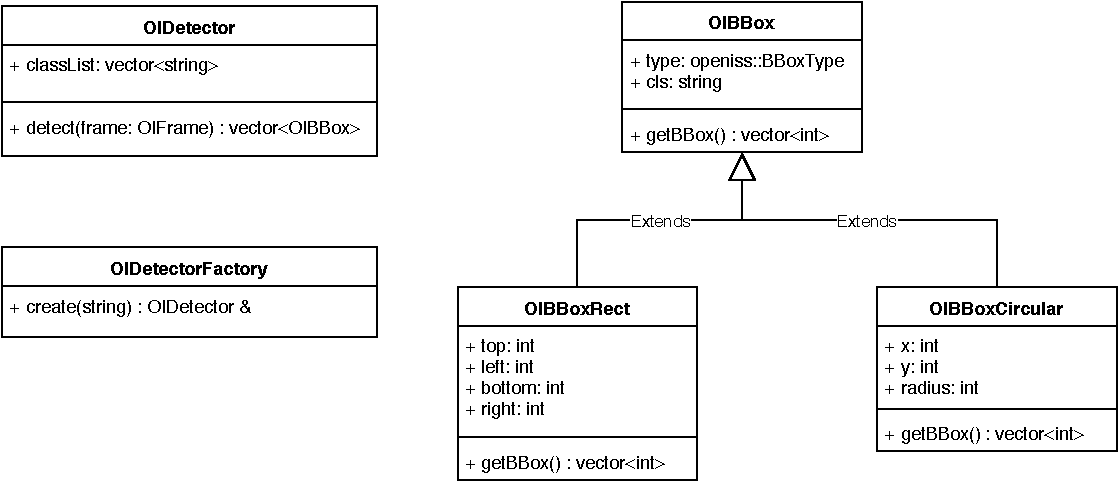
\includegraphics[width=\linewidth]{figures/framework_sub_detector.pdf}
    \caption{Design of the OpenISS detector specialized framework.}
    \label{fig:fw-sub-detector}
\end{figure}

\subsection{Recognizer Specialized Framework Design}
\label{sec:fw-design-spec-recognizer}

As mentioned in \autoref{sec:intro-pbstat}, our research problem can be divided
into two parts and we already explained object detection in the previous
section then the other one is object retrieval, more precisely, person
retrieval.
In other words, you are given a set of gallery images with their identities in
advanced. Then for a never seen query image, the recognizer is expected to tell
its identity among the gallery images.

Following the same pattern as the detector specialized framework, we design the
recognizer specialized framework shown as \autoref{fig:fw-sub-recognizer}.
Because we need to compare an item with all the items within a database, the
first step, of course, is that we need to create a database. According to our
definition, a database is a hashmap where the key is the identity string and
the value is a descriptor represented by the class \texttt{OIDescriptor}
computed from the source (e.g. an image or a video).
Inside the \texttt{OIDescriptor} class, the variable \texttt{srcPath} point to
the location of the source represented by this descriptor. The variable
\texttt{features} means the feature vector of the content of the source and the
variable \texttt{id} means the identity label.
Feature is one of the most significant parts for recognition, the core idea of
recognition is trying to find a way that can measure the distance between two
features accurately and effectively. Since these features are high dimensional
vector, it is hard to imagine and tell what kinds of metrics can perform better.
Feature is represented by the class \texttt{OINdArray} within the recognizer
specialized framework which encapsulates an N-dimensional array.
\texttt{OIRecognizerFactory} works exactly the same as its sibling within
the detector framework, we will omit the explanation for it here.
Finally, we reach the frozen spot of the recognizer representing by the class
named \texttt{OIRecognizer}. It has a variable name \texttt{database} which
holds all the pre-defined identities and three functions.
\texttt{attachDatabase} is easy to understand, as its name implies, it is used
to attach the database to the recognizer.
\texttt{lookupDatabase} defines how to look up the possible result
with a given descriptor in hand among the database.
\texttt{predict} is the method the user needs to invoke, it takes one parameter
typed \texttt{OIFrame} which is the image contains the targeted item.

\begin{figure}
    \centering
    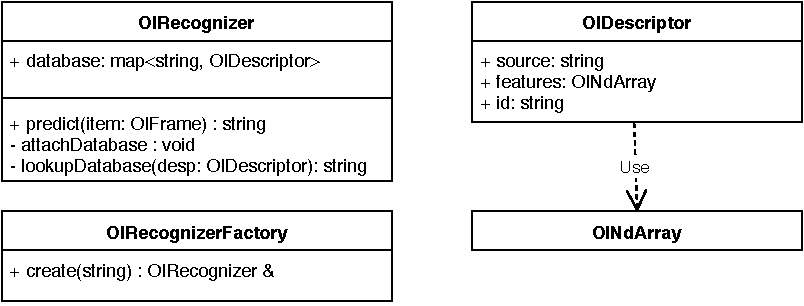
\includegraphics[width=\linewidth]{figures/framework_sub_recognizer.pdf}
    \caption{Design of the OpenISS recognizer specialized framework.}
    \label{fig:fw-sub-recognizer}
\end{figure}

\section{Summary}
\label{sec:fw-design-summary}

In this chapter, we introduced the design of our framework. Began with how
the framework solution can fulfill the requirement. Followed by the way how we
structure the framework, we logically split the whole solution into two parts,
one sever as infrastructure called core framework and the other one is
responsible for a specific task called specialized framework, in our design,
there can be multiple independent specialized frameworks.
Then we explained the design of each module (aka. frozen spot) within both the
core and specialized frameworks. In the next chapter, we are going to describe
how we create a framework instance to fulfill the requirements and scenarios
proposed in \autoref{sec:intro-scen-req}.

% EOF
\chapter{Framework Instantiation}
\label{chap:fw-inst}
\index{Framework Instantiation}

%%%%%%%%%%%%%%%%%%%%%%%%%%%%%%%%%%%%%%%%%%%%%%%%%%%%%%%%%%%%%%%%%%%%%%%%%%%%%%%%
\vspace*{-5mm}

In this chapter, we are going to describe in detail how we create an instance
of the framework we proposed in \autoref{chap:fw-design}. We start with the
implementation decisions by explaining why we choose the selected techniques
followed by the project structure used during the implementation time.
Then for each frozen spot introduced in \autoref{sec:fw-design-core} and
\autoref{sec:fw-design-spec}, we describe our instantiation process and the
essential implementation detail.

\vspace*{-2mm}
\section{Implementation Decision}
\label{sec:fw-inst-impl}
\vspace*{-2mm}

In \autoref{sec:fw-design-why}, we stated why we chose a framework design
approach. For a programming problem, if we just want to solve it and only it 
specifically, what we need may be just a piece of regular software. But if we want to
provide a generic solution that may apply to different problems, it requires extra work and may become more
complex. The framework approach aims at providing a general solution, so for
sure its complexity is higher and its development will become more difficult
than the usual approach.
Under such a situation, it is important to make decisions that can enable us to
work in an efficient and productive manner. For implementing a framework, what kind of
programming language we are going to use, how to compile the whole framework
with its dependencies and build executable software and how to manage the whole
project efficiently and clearly are all significant points that we have to address, 
which we are discussing in this chapter.

\subsection{Programming Language and Compilation Tool}
\label{sec:fw-inst-lang-ct}

In \autoref{sec:related_work_framework}, a list of currently available software
has been surveyed. From that list we found most of them were written in C++, based
on this fact, to make good used of the existing resources, we
determine to use C++ to develop our framework as well. We can benefit from using 
C++ in the following aspects:

\begin{itemize}
    \item Utilizes the existing software maximally.
    \item Obtains faster speed than most of the other programming languages 
    since it is closer to the hardware.
    \item Relatively easier to communicate with other languages since a many
    programming languages were themselves written in C/C++.
\end{itemize}

With these advantages, C++ also has it own limitations. For example, there is
no easy way to manage dependencies when the project becomes complicated.
To address this problem, CMake was selected, which is an open-source cross-platform building tool. By using it, we can build our framework in
Linux, MacOS or any other *nix-based platform with the same command.
Also, with the support of CMake, the end-users can enable the building process
partially which means they need only to compile and build the framework based on their
specific needs.

\subsection{Framework Layers and Project Structure}
\label{sec:fw-inst-layer-strcut}

In the context of software engineering, a system can be partitioned using the
concept of software layers. Software layers are where each ``layer" of a system
deals with a certain function of a system which, usually, gets more and more
detailed as you burrow down into the layer stack. In our implementation, to separate the responsibility of different modules and specialized
frameworks, we proposed a three-layer software model shown as
\autoref{fig:fw-layers} and assign components into
corresponding layers according to their functionalities, the description of each
layer can be found in \autoref{tab:desc-layer}. Within such a logically stated separation,
in our implemented code base, we also need to structure our code clear and
maintain the modularity of our design. For this purpose, we employ a project
directory structure shown as \autoref{tab:fw-dir}.

\begin{figure}
    \centering
    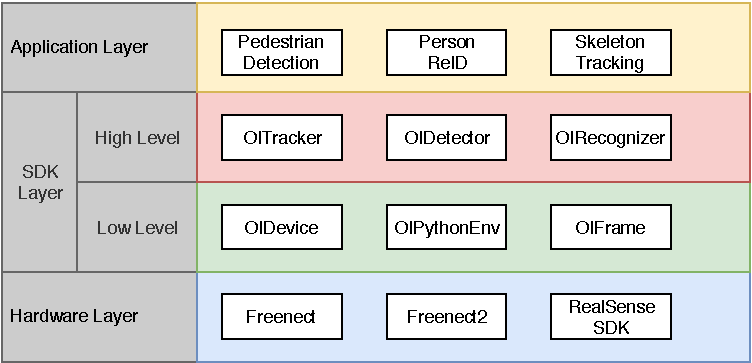
\includegraphics[width=\linewidth]{figures/framework_inst_layers.pdf}
    \caption{Three-layer model for OpenISS framework}
    \label{fig:fw-layers}
\end{figure}

\begin{table}
    \resizebox{\textwidth}{!}{%
    \begin{tabular}{ll}
        \hline
        \multicolumn{1}{c}{Layer's Name} & \multicolumn{1}{c}{Description} \\
        \hline
        Application Layer       & \begin{tabular}[c]{@{}l@{}}Provides sample
            usages of the framework for the end-users \\ (application
            developers)\end{tabular} \\ \hline
        SDK Layer (high level)  & \begin{tabular}[c]{@{}l@{}}Provides
            encapsulated functionalities to end-users, hide the \\ complexity
            of
            the implementation
        \end{tabular} \\ \hline
        SDK Layer (low level)   & \begin{tabular}[c]{@{}l@{}}Provides atomic
            APIs to the end-users which enable them to \\
            create custom functionalities based on their own demands
        \end{tabular} \\ \hline
        Hardware Layer          & \begin{tabular}[c]{@{}l@{}}Provides
            encapsulation of the hardware, which usually the application \\
            developers
            will not interested in
        \end{tabular}  \\ \hline
    \end{tabular}%
    }
    \caption{Description of the responsibility of different layers}
    \label{tab:desc-layer}
\end{table}

\begin{table}
    \resizebox{\textwidth}{!}{%
    \begin{tabular}{ll}
        \hline
        Directory Name &
        Description
        \\ \hline
        {\texttt{src}}       & Contains all the source code of the framework itself
        \\ \hline
        {\texttt{samples}}   & Contains all the source code of the application level
                    samples
        \\ \hline
        {\texttt{modules}}   & Contains custom cmake modules for building the framework
        \\ \hline
        {\texttt{python}}    & Contains all the python modules using by the framework
        \\ \hline
        {\texttt{script}}    & \begin{tabular}[c]{@{}l@{}}Contains all necessary
                    scripts (e.g. download datasets, \\ configure environment)
                    \end{tabular}
        \\ \hline
    \end{tabular}
    }
    \caption{Directory structure and their functionalities.}
    \label{tab:fw-dir}
\end{table}

\section{Framework Instantiation Overview}
\label{sec:fw-inst-core-and-spec-rel}

As discussed at the beginning of \autoref{sec:fw-design-spec}, the 
relationship between the core and specialized framework is that each
specialized framework takes the needed modules in the core as dependencies.
In this section, we would like to give an overview regarding how the instances 
we create will interact with the core and their corresponding specialized 
framework.

For the device instances, of course, it will have interaction with the
device module within the core. Precisely, the device instances will have to 
inherit the \texttt{OIDevice} class. Also, in order to allow the framework
to control the flow of execution, all the devices instance will have to
implement the \texttt{OIFlowable} interface.
For the tracker instance, two instances classes will have to inherit the
\texttt{OITracker} and the \texttt{OITrackerFrame} respectively.
For detector instance and recognizer instances, since our implementation are
based on deep learning approaches and the programs are written in Python.
First we have to inherit from the \texttt{OIDetector} and \texttt{OIRecognizer}
respectively, then take the \texttt{OIPythonEnv} as dependency. 
Finally, like the device module, they also have to implement the 
\texttt{OIFlowable} interface to transfer the control power to the core 
framework.

%When the framework being published, all the application developers will
%only use the exposed APIs which are defined in the core framework
%to build their applications. They cannot see the how the framework works
%internally which is the goal of encapsulation.

In the following section, we are going to explain in detail the instantiation
process of the essential device module within the core as well as each of the 
specialized frameworks.

\section{Core and Specialized Framework Instantiation}
\label{sec:fw-inst-core-and-spec}

In this section, we describe how we create hot spots for those frozen spots
introduced in \autoref{sec:fw-design-core} and \autoref{sec:fw-design-spec},
the augmented architecture diagram shown as \autoref{fig:fw-inst}.

For the device module in the core framework, we describe how we instantiate it 
to support three different kinds of depth cameras.
For the detector specialized framework, we describe what kind of modification we
made and how we train the YOLO model introduced in
\autoref{sec:related-worked-yolo} and integrate it into our solution as a
detector framework instance.
For the recognizer specialized framework, we describe how we train a person 
ReID network which is a combination of the identification model and triplet 
model explain in \autoref{sec:related-work-re-id-idm} and  
\autoref{sec:related-work-re-id-dism}.
For the tracker specialized framework, we describe how we instantiate it with 
the existing NiTE2 middleware introduced in 
\autoref{sec:related_work_openiss_nite2} implementation.

\begin{figure}
    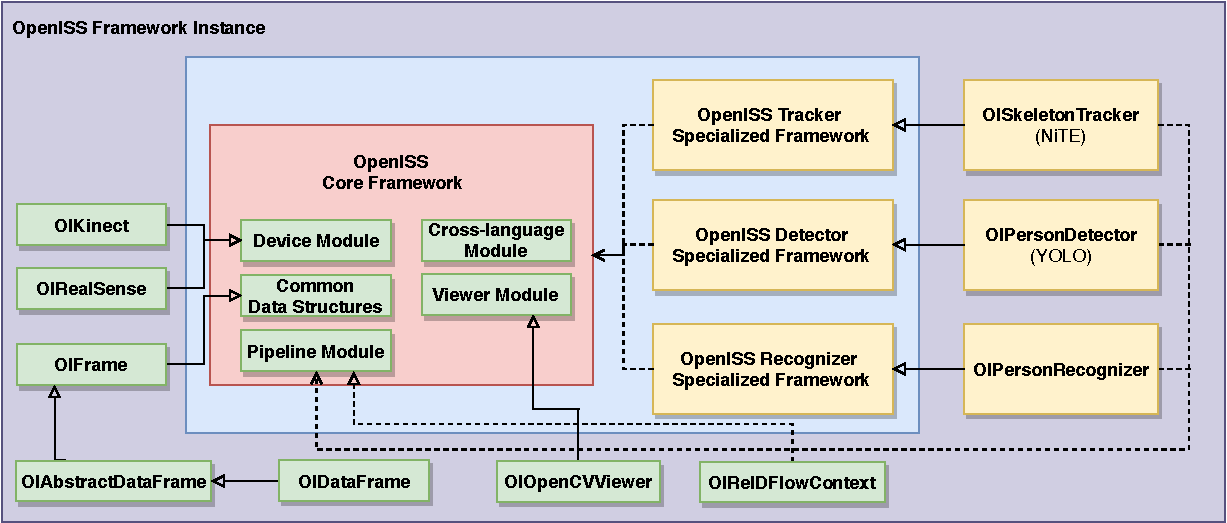
\includegraphics[width=\linewidth]{figures/framework_inst.pdf}
    \caption{Implemented OpenISS framework instance.}
    \label{fig:fw-inst}
\end{figure}

\subsection{Device Module Instantiation}
\label{sec:fw-inst-device}

In \autoref{sec:fw-design-core-device}, we described the design of the device
module within the core framework. To enable our framework to work with
real cameras, we have to instantiate the framework by creating a hot spot for 
the device's frozen spot.
Currently, we plan to support three kinds of devices: Kinect v1, Kinect v2 and
RealSense D435. These devices come from different manufacturers
which are supported by their own hardware drivers. To combine them within a same set of
APIs, the idea can be illustrated by \autoref{fig:fw-inst-device}. For each
kind of device, we create a concrete class, in our case, will be the class
\texttt{OIKinect} and \texttt{OIRealSense} to wrap the concrete implementation
of the defined functions within the \texttt{OIDevice} abstract class explained
in \autoref{sec:fw-design-core-device}.
Then because of the factory design pattern, what the framework users get from
the factory is a reference with type \texttt{OIDevice}, so they can obtain the
ability accessing the same function definition but with different implementation
from the dynamic dispatch mechanism.

\begin{figure}
    \centering
    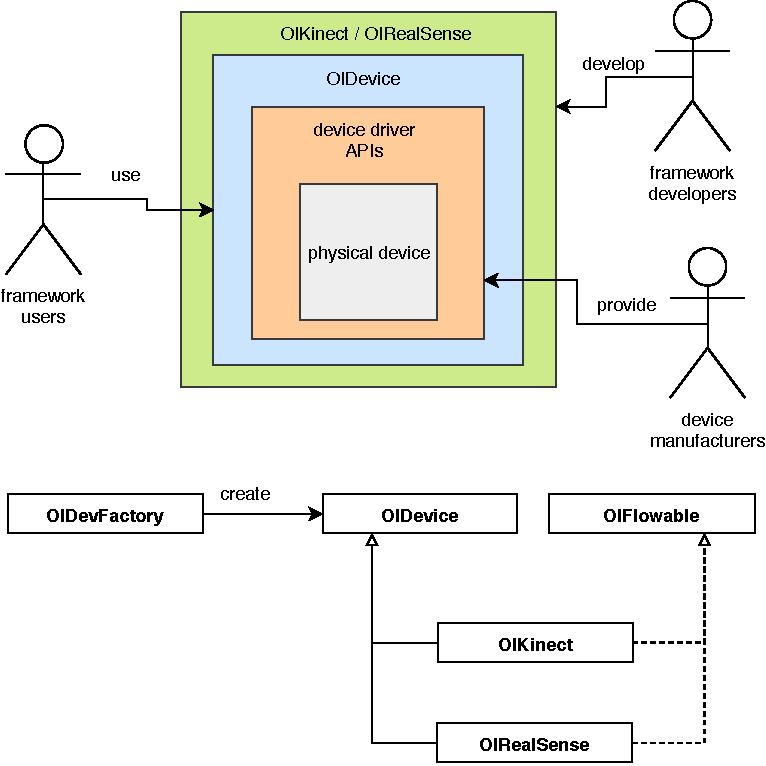
\includegraphics[scale=0.8]{figures/framework_inst_device.pdf}
    \caption{Instantiation of the device module of the core framework.}
    \label{fig:fw-inst-device}
\end{figure}

\subsection{Detector Specialized Framework Instantiation}
\label{sec:fw-inst-detector}

\begin{figure}
    \centering
    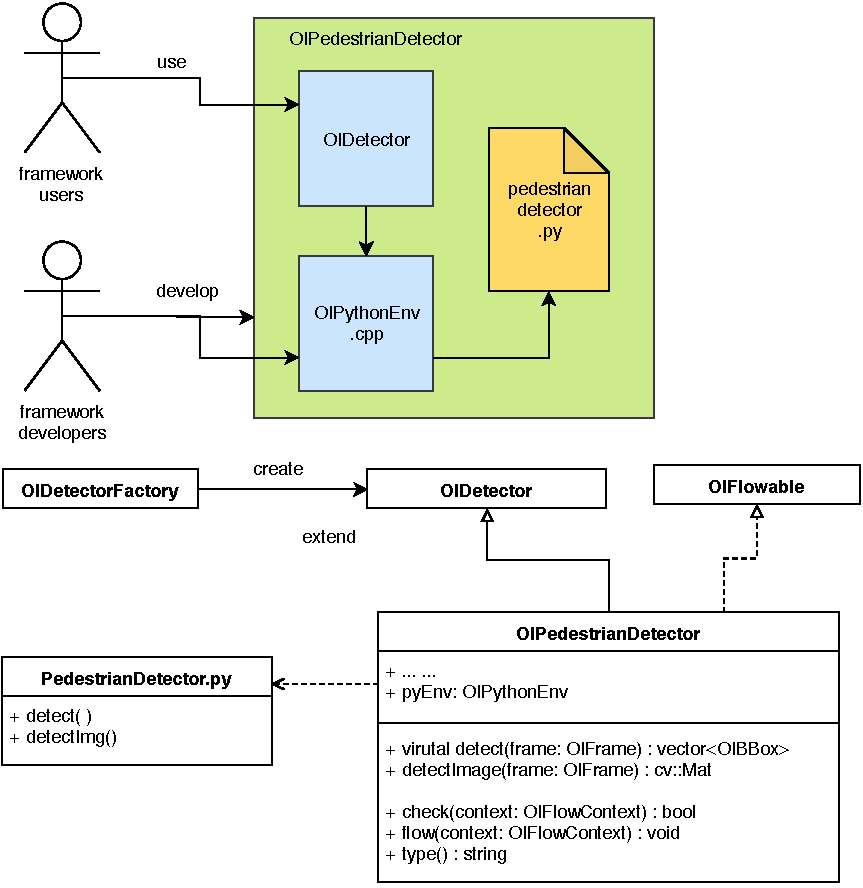
\includegraphics[scale=0.8]{figures/framework_inst_detector.pdf}
    \caption{Instantiation of the detector specialized framework.}
    \label{fig:fw-inst-detector}
\end{figure}

In \autoref{sec:fw-design-spec-detector}, we proposed the design of frozen spot
for a detector specialized framework in general. To achieve person
detection to fulfill our requirement, based on the detector frozen spot, we
create a deep learning-based person detector hot spot. The overall idea
shown as \autoref{fig:fw-inst-detector}.

We develop a concrete class \texttt{OIPedestrianDetector} which extends the
abstract class \texttt{OIDetector}, serving as a wrapper of the concrete Python
implementation of the YOLO detector. The communication required here between
C++ and Python is enabled by the cross-language module introduced in
\autoref{sec:fw-design-core-cross-lang} from the core framework.
From the users aspect, they don't need to worry about
how the framework works with various other detectors, but only need to know
the usage of them. For the specialized framework developers, 
with such design, they don't need to know how the cross-language works as well, 
but passing the requested methods or classes name to the \texttt{OIPythonEnv}, 
the cross-language module will handle it for you. It simplifies the required impementation
effectively by improving the effectiveness of the development process of both the applications and
framework itself.

We previously described the big picture of the detector specialized framework.
In the following paragraph, we will explain in detail how we implement the YOLO
model and reduce its scope from object detection to person detection.
%Recap the background \autoref{sec:intro-background} and requirements
%\autoref{sec:intro-mot-goal} we have, since we are doing performance on the
%stage, real-time data processing is extremely important for our application.
%According to \autoref{sec:related_work_obj_det} we know that
%two stages detector cannot achieve real-time (can only 5 FPS) so our
%selection for object detection model only left with the one-stage detector.
In this thesis, we take \cite{yolov3-keras-github} as a reference and training
facility, re-implement our version of the model since we want to adapt it to
our framework but use the trainer they provided to re-train the model.
The reason why we need to re-train is that the existing YOLO implementation
is used for object detection rather than person detection.
The difference between them is that if you want to make your model be able to
detect more classes of objects the more training time you need to
spend as well as memory space. Since we want to integrate two deep learning-based
approaches (detection and re-identification) in real-time, in such a context,
both time and space complexity are essential to us.

\begin{figure}
    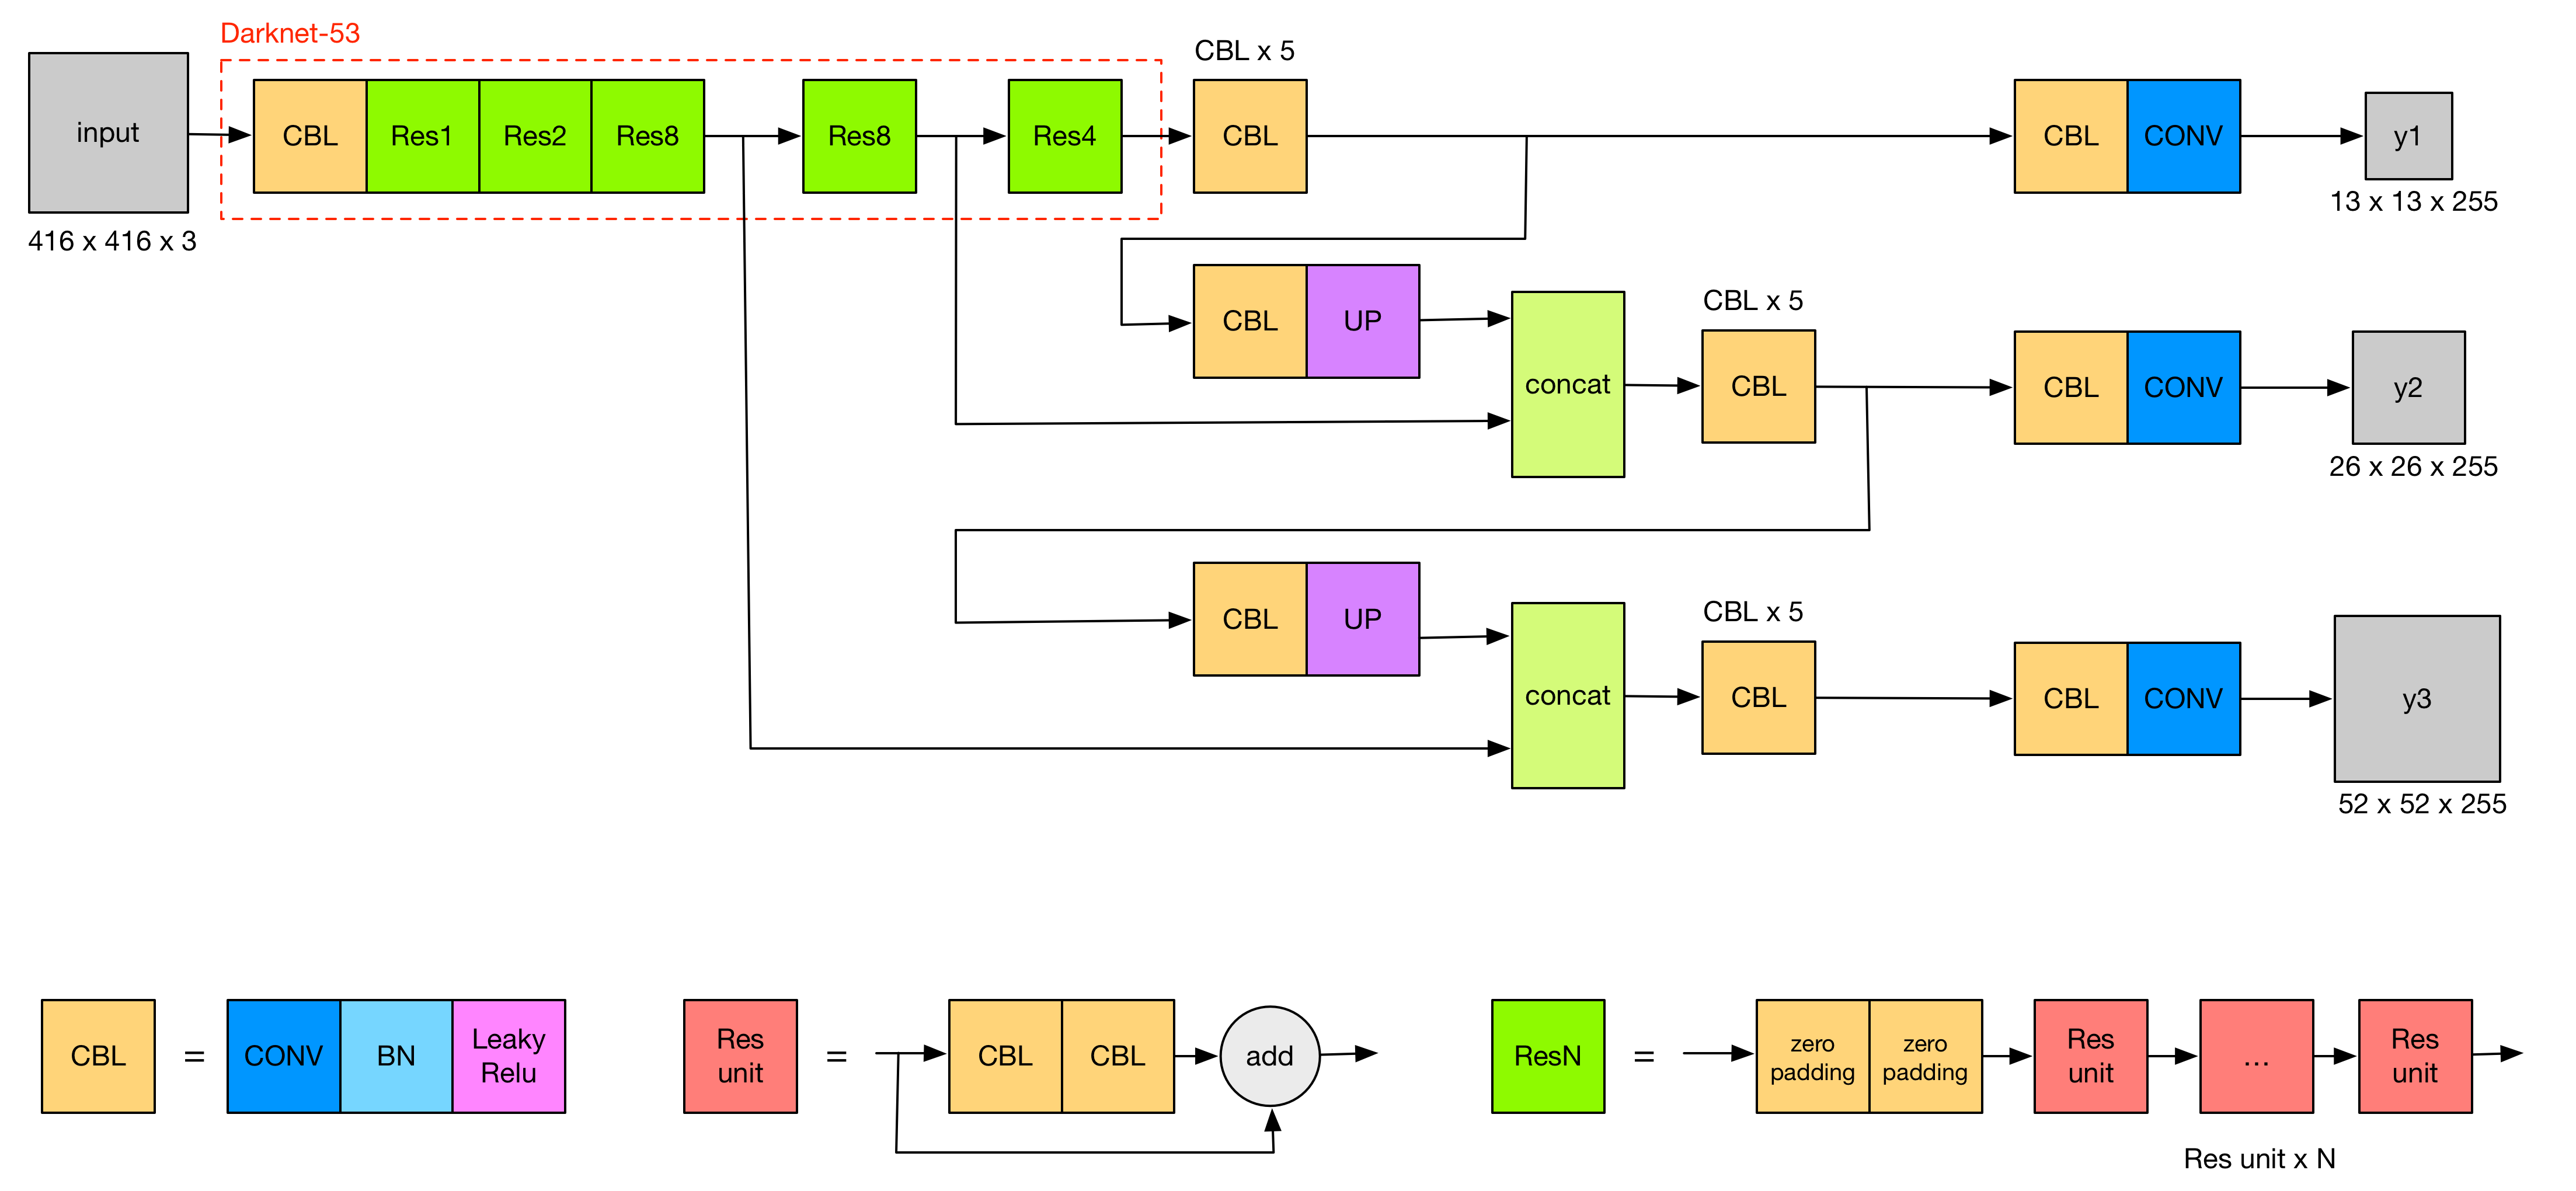
\includegraphics[width=\linewidth]{figures/framework_detector_archit.png}
    \caption{Implemented YOLO v3 architecture}
    \label{fig:fw-detector-archit}
\end{figure}

In our implementation, we follow exactly the same network architecture proposed
in \cite{yolov3-paper-2018} illustrated by \autoref{fig:fw-detector-archit}.
Since there are already numerous pre-trained YOLO model in existence, we are not going 
to train it from scratch, but perform some fine-tuning processes 
on a pre-trained model to get the one which can fit our need.
The full tuning process we employed can be described by the following steps:

\begin{enumerate}
    \item Download the well-trained YOLO model from its official repository.
    \item Convert the model's weight into Keras format from its original
    Darknet format.
    \item Download the VOC2012 dataset and loop over all images in the training
    set annotating the one with person(s) and extracting their corresponding
    bounding boxes information.
    \item Load the converted pre-trained weights then follow the methods
    proposed in the original YOLO v3 paper \cite{yolov3-paper-2018} to 
    fine-tune the model to obtain a person detector rather than an object
    detector.
\end{enumerate}

Since we reduce the complexity of an object detector to a person detector,
we believe that could help to improve the training speed. The following 
discussion explains our rationale:
According to \cite{yolov3-paper-2018}, there is a total of 9 anchors which are
obtained by applying K-means cluster algorithm during the training phase. 
These 9 anchors can be divided into 3 groups, each of them is given to final 
feature map with the size $[13, 13, 255]$, $[26, 26, 255]$ and $[52, 52, 255]$ 
respectively. 
So we can calculate that we are going to have:
$13 \times 13 \times 3 + 26 \times 26 \times 3 + 52 \times 52 \times 3=10647$
bounding boxes for each input image. For each bounding box, we need to compute
a probability for each of the pre-defined classes then multiply the confidence score 
for this box to obtain the final score for one class illustrated by
\autoref{fig:fw-detector-calc}. Take the VOC2012 dataset as
an example, there is a total of 20 classes of object. So for each bounding box,
there will be 20 times multiplication operations. Since we have 105647 boxes,
then it will be $20 \times 10647 = 212940$ operations per input image.
\textbf{
    But if we only care about the person we can reduce the 20 classes to 2
    classes, then the total calculation will be $2 \times 10647 = 21294$ which 
    is one-tenth of the original one. 
}
This can also speed up the non-maximum suppression (NMS) process which could 
help to eliminate overlapped boxes.
In most of the deep learning problems where the training data is normally large,
these modifications will significantly help to reduce the training time.

\begin{figure}
    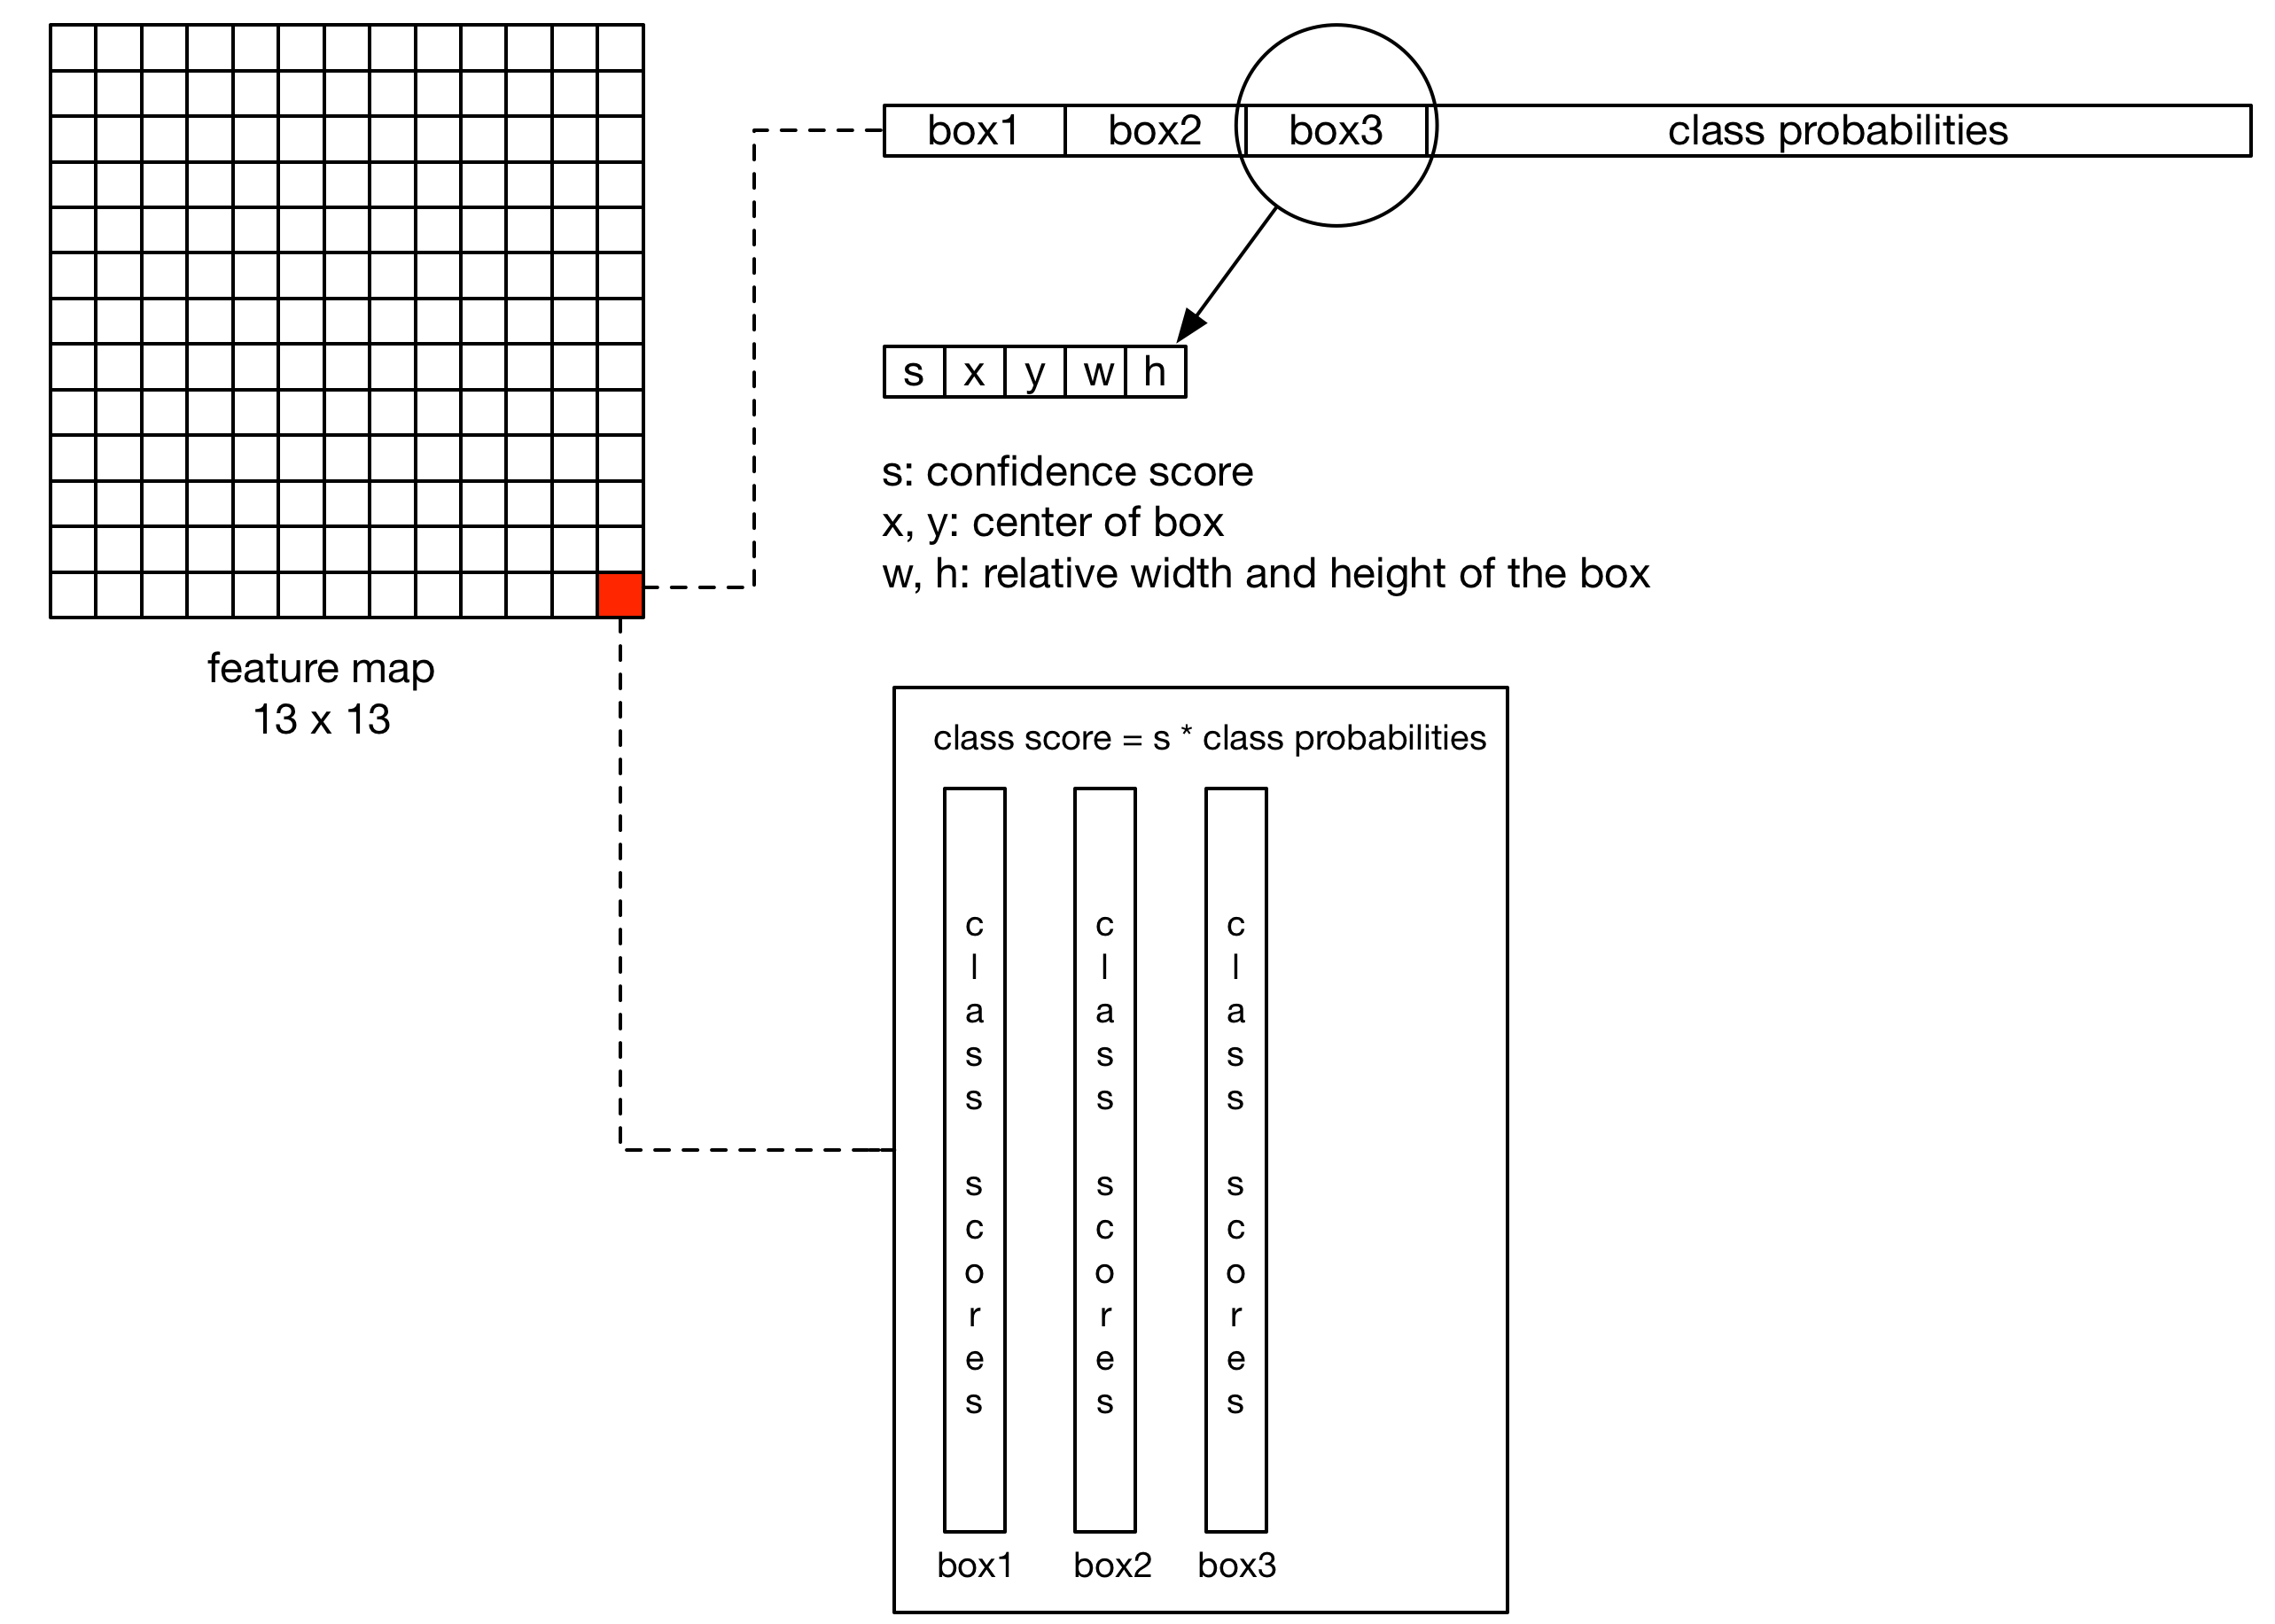
\includegraphics[width=\linewidth]{figures/framework_detector_calc.png}
    \caption{Calculation process of each cell in the feature map.}
    \label{fig:fw-detector-calc}
\end{figure}

Once we have the score for each interested class, we will (1) use a threshold to
filter out the one with a lower score and (2) apply the NMS algorithm to
eliminate the boxes with high overlapping ratio. Assume we still use the
VOC2012 dataset with 20 classes, since we have 10647 boxes, then the class score
can form a $20 \times 10647$ (row $\times$ col) matrix. The procedure can be
described in the following way and visualized by \autoref{fig:fw-detector-nms}.

\begin{enumerate}
    \item Examine all the class scores, select a $threshold$ then set all the
    score lower than $threshold$ to be zero.
    \item Take the class score for the same class from all predictive boxes,
    sort them in a decreasing order.
    \item Mark the box with maximum score as \texttt{bbox\_max}, then use it to
    compare with all the remaining boxes \texttt{bbox\_cur} on the intersection
    over union metric.
    \item if $IoU(\texttt{bbox\_max}, \texttt{bbox\_cur}) > 0.5$ then set the
    score to be zero. Otherwise, keep it unchanged.
\end{enumerate}

\begin{figure}
    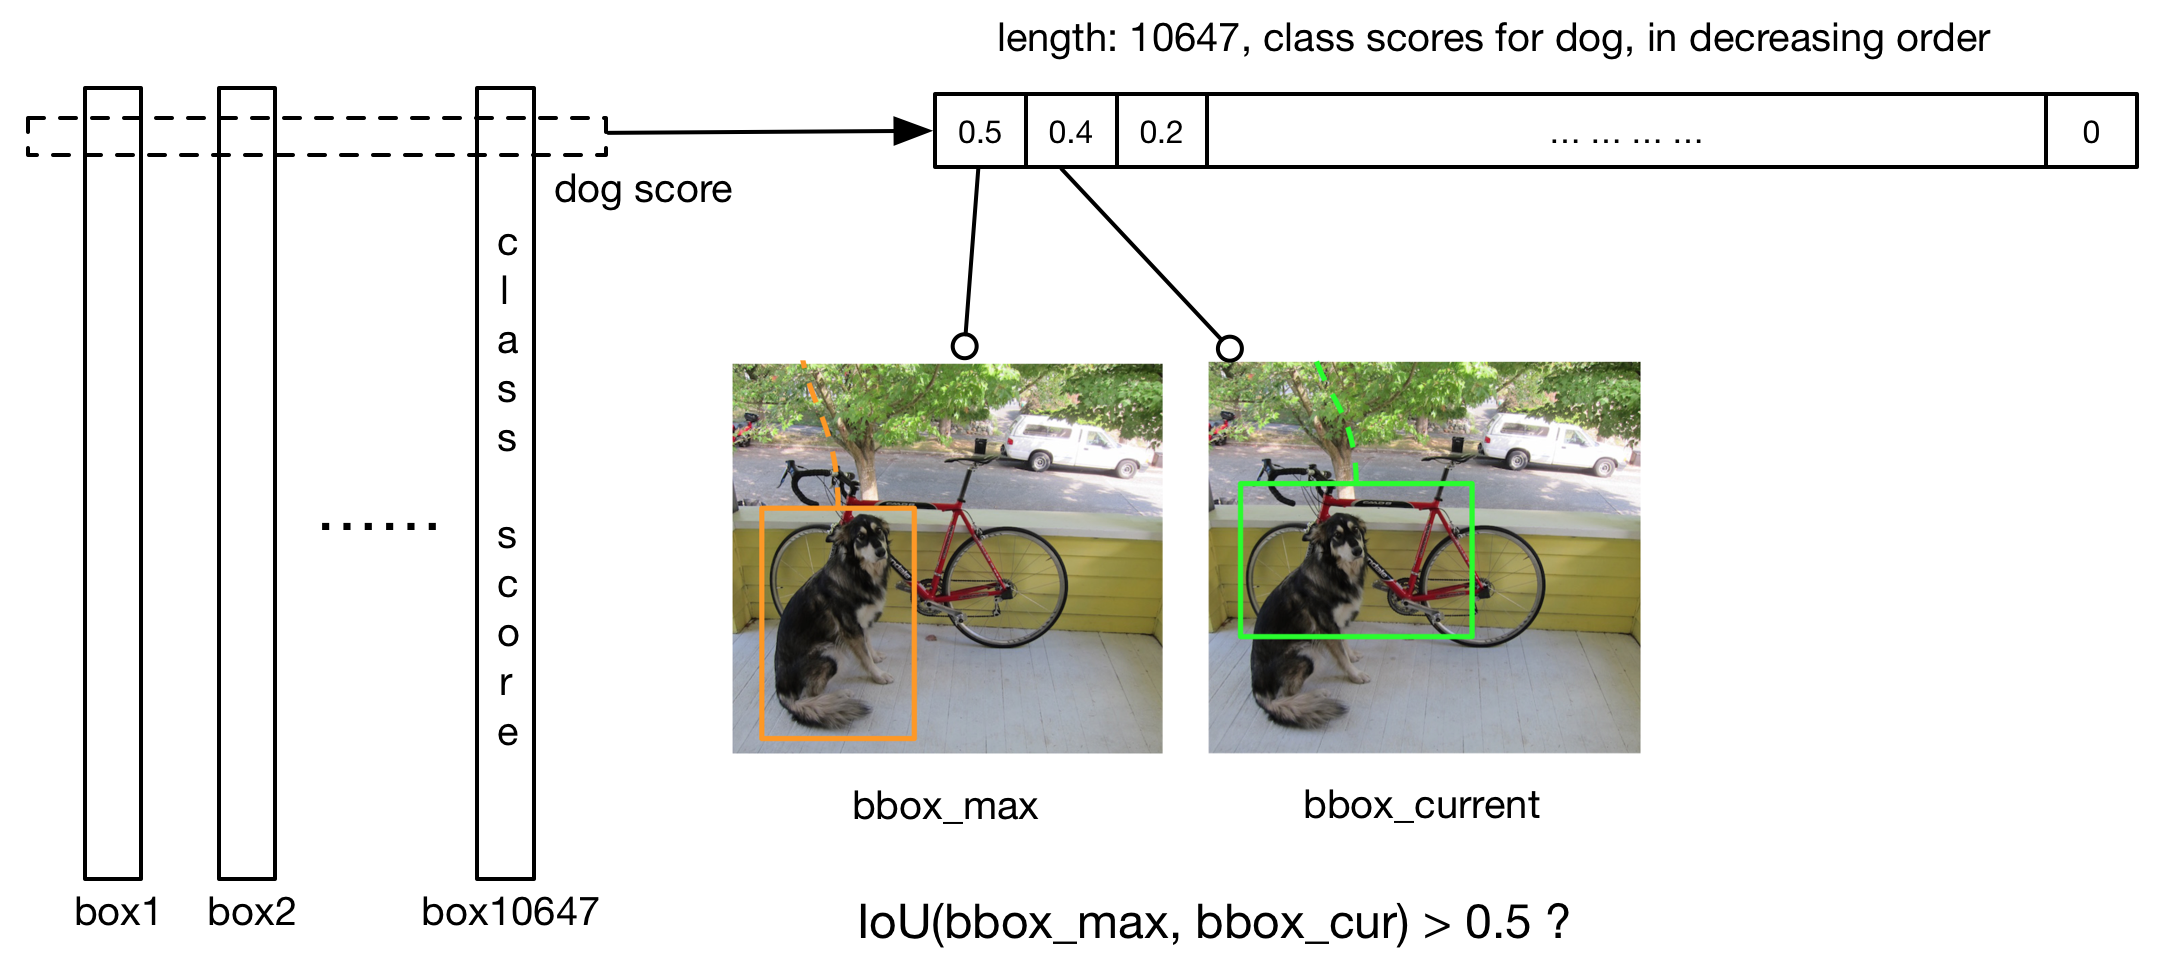
\includegraphics[width=\linewidth]{figures/framework_detector_nms.png}
    \caption{Non-maximum suppression process.}
    \label{fig:fw-detector-nms}
\end{figure}

\subsection{Recognizer Specialized Framework Instantiation}
\label{sec:fw-inst-recoginzer}

Person recognizer is the most significant component in our specialized
framework, without it we cannot reach our final goal covering the stage with
more than one camera. In \autoref{sec:fw-design-spec-recognizer}, we proposed the
generic design of the frozen spot for a common recognizer. For our specific
purpose, we need the capacity to re-identify the same person across multiple
cameras, so what we need is actually a person recognizer instance (hot spot).
Just like the way we did for the detector, we follow the same idea and come up with
the instantiation plan shown as \autoref{fig:fw-inst-recognizer}. The only
difference here is that the database invoked in this case, we have to create
the database first before we use the recognizer, otherwise, there is nothing to
be recognized. There is a variety of ways to create the database. The corresponding
logic should be added into the \texttt{attachDatabase} method. And the
comparison between the the input and the records within the database should be written in
the method \texttt{lookupDatabase}. In this case, we are using a deep
learning-based model, so we need to use the model to compute the
descriptor for each given record and store them in the database then compare the
distance between query and gallery descriptors. More detail can be found in
\autoref{fw-recognizer-spec-inference}.

\begin{figure}
    \centering
    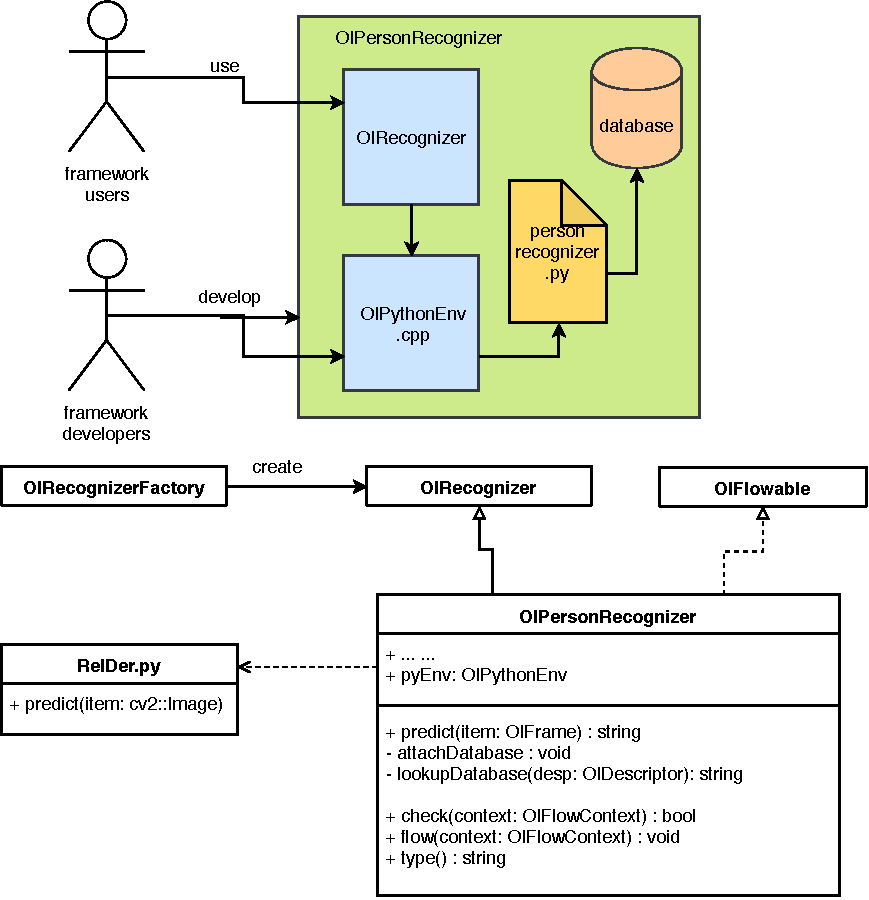
\includegraphics[scale=0.8]{figures/framework_inst_recognizer.pdf}
    \caption{Instantiation of the recognizer specialized framework.}
    \label{fig:fw-inst-recognizer}
\end{figure}

In order to keep the consistency with the person detector and fill the
research gap described in \autoref{sec:related_work_openiss_tf}, our 
implementation of the recognizer is written in Python and built on top of 
TensorFlow and Keras.
In the following paragraph, we first introduce our network structure, then
explain our training process which includes data pre-processing, loss 
function,  optimizer and some important hyper-parameters.
In the end, we will discuss the methodology that we used to perform inference
by using the trained model.

\subsubsection{Network Architecture}
\label{fw-recognizer-spec-network-arch}

\begin{figure}
    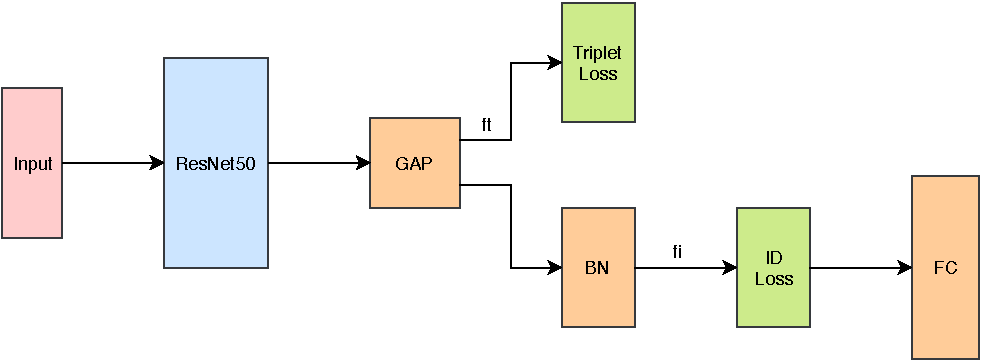
\includegraphics[width=\linewidth]{figures/framework_reid_archit.pdf}
    \caption[Implemented recognizer network architecture]
    {
        Implemented recognizer network architecture.
%        GAP: global average pooling layer, BN: batch normalization
%        layer, FC: fully connected layer.
%        $f_t$: features used to calculate triplet loss,
%        $f_i$: features used for inference.
        The pink color represents input, blue means backbone network, orange
        represents a special layer and green means loss function layer.
    }
    \label{fig:fw-reid-archit}
\end{figure}

We implemented a network architecture shown as \autoref{fig:fw-reid-archit},
which is a combination of the identification model and distance metric-based
model mentioned in \autoref{sec:related_work_re_id}. It employs a Residual-50
network as the feature extractor followed by a global average pooling layer
(GAP) to flatten out the feature vector. Then in one branch, the extracted
feature $f_t$ was sent to calculate the triplet loss while in
the other branch was used to obtain $f_i$ after passing through a batch 
normalization layer (BN) to compute the identification loss. 
In the end, the fully connected
layer (FC) is responsible for classification during the training time.
According to \cite{pcb-and-rpp-for-reid},
if we can get a higher spatial resolution before global pooling by changing the
stride in the last convolutional layer from 2 to 1, which would not affect the
number of parameters, obvious improvement can be obtained. Because of that, we
modified our ResNet50 accordingly. Like most of the deep learning tasks, our
model was also initialized with the weights pre-trained on ImageNet.
From the implementation point of view, it is important
to point out that when we are using any pre-trained weights, we need to make
sure the input image respect to the format of the pre-trained model. In Keras,
this can be done by invoking the \texttt{preprocess\_input} method within the
pre-defined model package.

\subsubsection{Training}
\label{fw-recognizer-spec-train}

As we can see from \autoref{fig:fw-reid-archit}, during the training, our model
will be guided by two loss functions: triplet loss and ID loss.

%\begin{equation}
%    L = L_{triplet} + \beta L_{center} + L_{ID}
%\end{equation}

\begin{equation}
L = L_{triplet} + L_{ID}
\end{equation}

\noindent where $L_{triplet}$ is defined as \autoref{eq:common-triplet-loss},
$L_{ID} = - \mathbf{y} \cdot \log(\mathbf{\hat{y}})$
is the cross-entropy loss.
% and $L_{center} = \frac{1}{2} \sum_{j=1}^{B}
%\norm{f_{t_j} - c_{y_i}}^2_2 $ represents the center loss
%\cite{center-loss-2016}. In our implementation, $\beta$ is set to 0.0005.

Since the training set is too large to fit into memory in one shot,
the mini-batch training strategy was adopted as well as
the sampling method proposed in \cite{in-defense-of-triplet-loss-for-reid-2017}.
For each mini-batch, we randomly select $P$ identities and for each identity 
random $K$ images will be chosen. In our implementation,
$P$ is set to 16 and $K$ is set to 4, which makes the batch size to become 64.
This work is done by the class \texttt{RandomSampler} whose UML diagram shown as
\autoref{fig:fw-sampler-uml}.

In order to prevent overfitting and enhance the generalization ability of the
model, a data augmentation technique named random erasing
\cite{random-erasing-data-augmentation-2017} was applied to each image
individually on-the-fly when constructing each mini-batch of data. Just like its
name suggests, it will randomly replace a portion of the pixel's intensity 
within the image with some random values. 
Besides that three more steps pre-processing
were applied to enlarge the dataset. These pre-processing methods are commonly
used in the image-based deep learning problem, they are implemented in the file
named \texttt{preprocess.py}.

\begin{itemize}
    \item Pad 10 pixels around the image
    \item Randomly crop the image back to the size before padding
    \item Flip the image horizontally with 0.5 probability
\end{itemize}

For the optimizer, we used the build-in Adam algorithm provided by Keras
but with warm-up learning rate setting \cite{learning-rate-warmup-2018}.
Precisely, the learning rate has been scheduled as \autoref{eq:reid-lr}, where 
$t$ is the current epoch. Last but not least, according to
\cite{tricks-and-baseline-for-reid-2019}, they trained their model for 120
epochs and it is sufficient to obtain a good result. Also, from our training
result shown by \autoref{fig:fw-training}, this number is enough for the
model's convergence, so we set our total training epochs to 120 as well.

\begin{equation}
\label{eq:reid-lr}
\operatorname{lr}(t)=\left\{
\begin{array}{ll}
{3.5 \times 10^{-5} \times \frac{t}{10}} & {\text { if } t \leq 10} \\
{3.5 \times 10^{-4}} & {\text { if } 10<t \leq 40} \\
{3.5 \times 10^{-5}} & {\text { if } 40<t \leq 70} \\
{3.5 \times 10^{-6}} & {\text { if } 70<t \leq 120}
\end{array}\right.
\end{equation}

\begin{figure}
    \begin{center}
        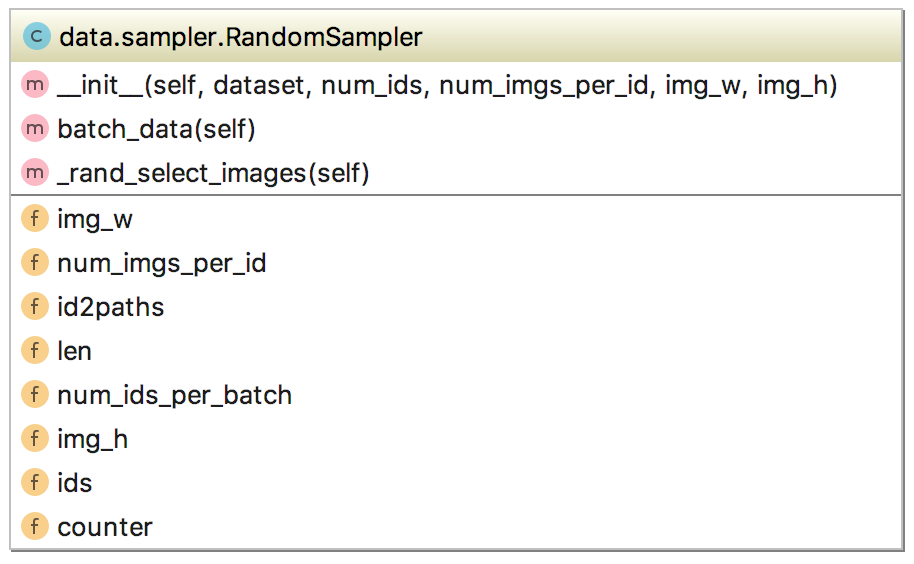
\includegraphics[scale=0.6]{figures/framework_reid_sampler_uml.png}
    \end{center}
    \caption{UML class diagram of \texttt{RandomSampler} class}
    \label{fig:fw-sampler-uml}
\end{figure}

From the implementation point of view, the training program can be illustrated by
\autoref{fig:fw-reid-code-overview}. Firstly, we defined a set of configuration
variables and the structure of the model. Then we pass the configuration to the
model, attach it with defined loss functions, optimizer and necessary
callback functions then run the model in training mode. During the training
time, the data will be retrieved from the dataset, sampled by the
\texttt{Sampler}, applied data argumentation by \texttt{DataGen} and wrapped
up to be a Python generator object by \texttt{DataGenWrapper}.

With these setting and after training, the result can be visualized by
\autoref{fig:fw-training}, we can see clearly that the model starts to converge
at around $50^{th}$ epochs. And from the training accuracy figure, we can find
that there is a steep increase between $10^{th}$ and $20^{th}$ epochs.

\begin{figure}
    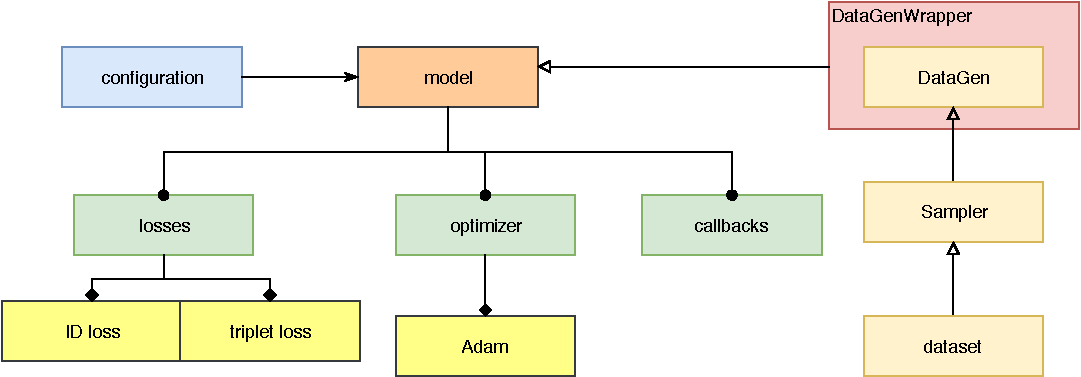
\includegraphics[width=\linewidth]{figures/framework_reid_code_overview.pdf}
    \caption{Code structure of the ReID training program}
    \label{fig:fw-reid-code-overview}
\end{figure}

\begin{figure}
    \begin{subfigure}
        \centering
        \includegraphics[width=.5\linewidth]{figures/train_id_loss.png}
    \end{subfigure}
    \begin{subfigure}
        \centering
        \includegraphics[width=.5\linewidth]{figures/train_triplet_loss.png}
    \end{subfigure}
    \begin{subfigure}
        \centering
        \includegraphics[width=.5\linewidth]{figures/train_loss.png}
    \end{subfigure}
    \begin{subfigure}
        \centering
        \includegraphics[width=.5\linewidth]{figures/train_acc.png}
    \end{subfigure}
    \caption[Training visualization diagram]
    {Training visualization diagram. Upper left: training identification loss
        curve. Upper right: training triplet hard loss curve. Lower left: total
        training loss curve. Lower right: training classification accuracy.}
    \label{fig:fw-training}
\end{figure}

\subsubsection{Inference}
\label{fw-recognizer-spec-inference}

We explained the training process above, let's take a look at the inference
procedure. Assume we have a query image $q$ and a set of gallery images $G$.
The model is denoted by $M$ and the output of model will be $f_i$ then we have:

$$
f_i^{query} = M(q) \:\:\: \text{and} \:\:\: f_i^{G} = M(G)
$$

Once we have the feature descriptor, then for each $f \in f_i^G$  we calculate
the distance $D_i$ between $f$ and $f_i^{query}$:

\begin{equation}
\label{eq:dis-comp}
D_i =  distance(f, f_i^{query}) \:\: f \in f_i^G
\end{equation}

Finally, the gallery image which gives the minimal distance will be the one
whose identity needs to be returned:

$$
id = \arg \min(D_i)
$$

If the reader wants to reproduce the result, attention needs to be paid on one issue
that the dimension of $f_i^{query}$ and $f_i^G$ are different so when we try
to feed the single query image into the model, we have to explicitly add one
more axis to it.
What's more is that, according to \autoref{eq:dis-comp},  a $distance$ function is
used to perform comparison between $f$ and $f_i^{query}$. The most popular
distance function for two vectors comparison are: (1) euclidean distance and (2)
cosine distance. According to \cite{tricks-and-baseline-for-reid-2019}, using
(2) can obtain a better result. Our implementation offers both two
methods, but for simplicity we don't follow exactly the cosine distance
calculation. We have the function \texttt{euclidean(f1, f2)} for the standard
Euclidean distance but \texttt{L2(euclidean(f1, f2))} which is equivalent to cosine distance.

\subsection{Tracker Specialized Framework Instantiation}
\label{sec:fw-inst-tracker}

In the plan of OpenISS framework, there are three kinds of trackers that are needed:
skeleton tracker, facial landmark tracker and gesture tracker. In this thesis,
we focus on the skeleton tracker.
Skeleton tracking is the processing of depth image data to establish the
positions of various skeleton joints on a human form. This information can be
useful in many cases, as mentioned in \autoref{sec:related_work_other},
the approach proposed by \cite{rgbd-for-reid} takes skeleton as the starting
point. A lot of research has been conducted in this area and a lot of
methods both conventional and deep learning-based have been developed. We will
not focus on developing our own approach but to implement an existing one and design it as an
instance of the specialized framework to allow users to integrate other approaches or
develop their own approach easily.

Like what we did for the device abstraction, here we design a similar mechanism
which is a hierarchical architecture shown as \autoref{fig:fw-skeleton-tracker}
that can support real-time skeleton tracking with good extensibility without
any GPU device needed.
From the implementation point of view, firstly, we abstract the common
functionalities of the skeleton tracker to create an abstract superclass
\texttt{OITracker}, which serves as a contract exposed to the users and hides its
implementation complexity.
Our implementation is based on a middleware of OpenNI2 named NiTE2
mentioned in \autoref{sec:related_work_openiss_nite2}. So we create a concrete
subclass which inherits from \texttt{OITracker} named \texttt{OINiTETracker}.
It can be seen as an adapter that adapts the NiTE tracking algorithm to our
framework's data structure.
Let's go deeper, starting from the method \texttt{readFrame(OITrackerFrame)}.
Every time a new frame is read from the device, this method will be
invoked. Its job is to perform skeleton detection to take the data from the
NiTE2's data structure and move them to several OpenISS framework's data
structures which will be eventually packed into \texttt{OITrackerFrame}.
There are three specialized framework-specific data holder classes and their
responsibilities listed below:

\begin{itemize}
    \item \texttt{OIUserData} contains all the data for each single
    detected skeleton.
    \item \texttt{OIUserMap} contains a 2d array with the same resolution
    as the depth image, where the background indicated by 0 and the detected
    skeleton for each person indicated by their user id.
    \item \texttt{OISkeleton} contains a hashmap which the key is the joint
    type and the value is the position of that joint.
\end{itemize}

\begin{figure}
    \centering
    \includegraphics[scale=0.7]{figures/framework_inst_tracker.pdf}
    \caption{Instantiation of the tracker specialized framework.}
    \label{fig:fw-skeleton-tracker}
\end{figure}

\subsection{ReID Context Instantiation}
\label{sec:fw-inst-context}

As mentioned in \autoref{sec:fw-design-core-pipeline}, we have the pipeline
module designed in the core framework. In this chapter, we have
\texttt{OISkeletonTracker}, \texttt{OIPedestrianDetector} and
\texttt{OIPersonRecognizer} both implementing the \texttt{OIFlowable} interface to
serve as filters within a pipeline. In order to build up a ReID pipeline for
our final goal, what we are still missing is a concrete class for the
\texttt{OIFlowContext} which will be used as the data holder for intermediate
result generated during the execution of the pipeline.
For this purpose, we define a class \texttt{OIReIDFlowContext} which extends
the abstract class \texttt{OIFlowContext}.
For ReID task, the pipeline will need to contain
the concrete implementation of a device, a detector, a recognizer and a viewer.
Also, all the input and output of these components are
being defined in the previous sections. So within the concrete context class,
we need to define the way we store the temporary results. For example, the
data frame captured from the device, the bounding boxes used to mask out the
detected person, as well as the way we query them from the latter filter within
the pipeline.
In this case, since we have the \texttt{type} of each filter and all of them
are distinct from each other, we use their type as a key and create
different logic when the \texttt{query} or \texttt{save} get called within
their respective implementation as a pipeline filter.

\section{Summary}
\label{sec:fw-inst-summary}

In this chapter, we describe the instantiation and implementation for the
frozen spots within both the core and specialized frameworks. A lot of focus is
put on discussing two deep learning-based models' development (detector and
recognizer) as well as how to integrate them into the specialized framework
with the desired APIs exposed.
In the next chapter, we will see how can we make use of these hot spot classes to form an
application which can eventually address our research problem.
% EOF

\chapter{Applications}
\label{chap:fw-app}
\index{Application}

%%%%%%%%%%%%%%%%%%%%%%%%%%%%%%%%%%%%%%%%%%%%%%%%%%%%%%%%%%%%%%%%%%%%%%%%%%%%%%%%
In this chapter, we will explain in detail how to make use of the framework
instance we created in \autoref{chap:fw-inst} to build a person
re-identification application to realize tracking the same person across
multiple cameras. Besides the main ReID application, we will also introduce other
applications: skeleton tracking, camera calibration, image alignment
and green screen image, which are all built on top of our OpenISS framework. With the
applications added, the architecture of our current system can be shown by
\autoref{fig:fw-app}.

\begin{figure}
    \centering
    \includegraphics[width=\linewidth]{figures/framework_app.pdf}
    \caption{Applications built on top of our framework instance.}
    \label{fig:fw-app}
\end{figure}

\section{ReID Application}
\label{sec:fw-app-reid}

In \autoref{sec:fw-design-spec-detector} and
\autoref{sec:fw-design-spec-recognizer}, we stated the design of the detector
and recognizer frozen spot. In \autoref{sec:fw-inst-detector} and
\autoref{sec:fw-inst-recoginzer}, we described how we create hot spot for the
detector and recognizer adapting to the specific pedestrian detection and
person retrieval tasks. Also, they all agree with the \texttt{OIFlowable}
interface to support the pipeline mechanism defined in the core framework.
In this section, we are going to explain, how we use the framework instance
described in \autoref{chap:fw-inst} for person re-identification task by
chaining the proposed hot spots together which is supported by the pipeline module.

\begin{figure}
    \centering
    \includegraphics[width=\linewidth]{figures/framework_app_reid_pipeline.pdf}
    \caption[Person re-identification pipeline]
    {Person re-identification pipeline,  the solid line arrow represents
    the pipeline execution order and the dash line arrow represents the
    data flow.}
    \label{fig:fw-app-reid-pipeline}
\end{figure}

As mentioned in \autoref{sec:intro-pbstat}, the person ReID task can be divided
into two portions one is person detection and other is person retrieval. Since
we already have these two specialized framework instances. Intuitively, what we
need to do is just arrange them in a suitable order to make them work properly.
With such consideration, we propose the ReID pipeline shown as
\autoref{fig:fw-app-reid-pipeline}, which works in the following manner:

\begin{enumerate}
    \item The raw data flow into the device module from the core framework and
    being encapsulated as an instance of \texttt{OIFrame}.
    \item The frame then being passed to the pedestrian detector which is a
    concrete implementation of the abstract \texttt{OIDetector} class invoking
    the deep learning-based model implemented in Python via the cross-language
    module in the core.
    \item The output of the detector specialized framework will be a list of
    bounding boxes which can use to mask the data frame, each these mask
    contains the appearance of a person.
    \item These results will flow into the recognizer specialized framework
    which again depends on cross-language module since the corresponding
    model is also implemented in Python to compare the descriptor among the
    database.
\end{enumerate}

As mentioned in \autoref{sec:fw-design-core-pipeline}, the \texttt{OIPipeline}
serves as the execution engine for a list of filters, it will call the first
one then passing the result one after another. So the entry point of the
application will be the \texttt{flow} method defined in the \texttt{OIFlowable}
interface which is part of the core framework. What the user needs to do is
telling the framework how to assemble the filters within the pipeline. That is
done by creating an instance of the \texttt{OIFlowable} object and invoking the
\texttt{push} method defined in \texttt{OIPipeline} class to add that object in
the pipeline.
Then the framework will take the flow of control within the pipeline, the data
from the device will be flowed into the pushed filters one by one.
The steps we describe here can be accurately expressed by
\autoref{algo:fw-app-reid}.

\begin{algorithm}
    devF $\leftarrow$ create a device factory\;
    detF $\leftarrow$ create a detector factory\;
    recogF $\leftarrow$ create a recognizer factory\;
    db $\leftarrow$ create a database for recognizer\;
    \;
    noEcsPressed = True\;
    device = devF.create("name of the device")\;
    detector = detF.create("name of detector")\;
    recognizer = recogF.create("name of recognizer")\;
     recognizer.attachDatabase(db)\;
    \;
    reidContext = new OIReIDFlowContext \;
    reidPL = new OIPipeline(reidContext) \;
    reidPL.push(dev)\;
    reidPL.push(detector)\;
    reidPL.push(recognizer)\;
    reidPL.push(new OIOpenCVViewer)\;
    \;
    \While{noEcsPressed}{
        reidPL.flow(reidContext)\;
        \If{isEcsPressed}{
            noEcsPressed = False\;
        }
    }
    \caption{ReID application procedure}
    \label{algo:fw-app-reid}
\end{algorithm}

It is important to notice how the pipeline mechanism works by looking carefully
through this application. The user calls a function defined in the core, then
the framework gives the result back without any user interaction according to the
pipeline the user assembled which is actually the beauty of the framework
solution.
It frees the user from knowing how they need to handle the temporary result, in
this case, what the user want is a working ReID application, they are not
interested in the person detection or any other thing else. With the pipeline
module or we can say the framework solution, the user just needs to tell what
they want and the framework will take care of the rest and return the result
directly. Also, it enables us to design each specialized framework modularly and
make these components reusable.

In our design, the pipeline module resides in the core which doesn't know
anything about the specialized frameworks. But with the interface defined,
it enables the hot spot which may be created the latter to make use of the pipeline.
All the thing need to be done is creating an instance of the context.
Because of the fact that the pipeline only contains the type of abstract
class and the data flow is defined by the abstract methods, it will not affect
the final functionality of the pipeline but makes the it pluggable and robust.

\section{Skeleton Tracking}
\label{sec:fw-app-skt}

As mentioned in \autoref{sec:intro-sq-skt}, we would like to keep the
functionality of skeleton tracking originally designed for ISSv2. To achieve
that, We define a set of frozen spots in \autoref{sec:fw-design-spec-tracker}
and create a specific hot spot for these frozen spots by adapting the
implementation from NiTE2 in \autoref{sec:fw-inst-tracker}.

The workflow of the tracker instance shown as \autoref{fig:fw-skeleton-workflow}.
Firstly, the tracker factory \texttt{OITrackerFactory} will take a concrete
class of \texttt{OIDevice} and create the instance of a concrete tracker but
return a reference of its superclass \texttt{OITracker}. Secondly, the tracker
will aggregate the information from NiTE2 and update the data holder within
the concrete class of \texttt{OITrackerFrame}, in our case,
\texttt{OINiTETrackerFrame}. Finally, the gathered data will be sent to
the viewer and draw the skeleton out for the user.
In \autoref{fig:fw-skeleton-workflow}, the box in orange (NiTE2) is one of the
possible implementation. It can be replaced by any other implementation by
passing different indicators to the tracker factory.

\begin{figure}
    \includegraphics[width=\linewidth]{figures/framework_oitracker_workflow.png}
    \caption[Tracker module interactive diagram]
    {Tracker module interactive diagram,
        the boxes in blue are our framework's components, the box in
        orange is the concrete tracking algorithm implementation, the boxes in
        gray are the low level components.}
    \label{fig:fw-skeleton-workflow}
\end{figure}

In \autoref{sec:fw-inst-tracker}, we show that the \texttt{OISkeletonTracker}
class also agree with the \texttt{OIFlowable} interface which means that the
skeleton tracking application will work in the same manner as our ReID
application. With the pipeline mechanism introduced, our first step will be
creating a corresponding skeleton tracking pipeline shown as
\autoref{fig:fw-app-skt-pipeline}, then we instantiate the a device filter as
input, a tracker filter to perform tracking and a viewer filter for display.
Next, as what we did for ReID application, we have to create a concrete
\texttt{OIFlowContext} for the skeleton tracking task named
\texttt{OISktFlowContext}.
Finally, invoke the \texttt{flow} method of the pipeline instance.
The procedure can be described as \autoref{algo:fw-app-skt}.

\begin{figure}
    \centering
    \includegraphics[width=\linewidth]{figures/framework_app_skt_pipeline.pdf}
    \caption[Skeleton tracking application pipeline]
    {Skeleton tracking application pipeline, the solid line arrow represents
    the pipeline execution order and the dash line arrow represents the
    data flow.}
    \label{fig:fw-app-skt-pipeline}
\end{figure}

\begin{algorithm}
    devF $\leftarrow$ create a device factory\;
    tkF $\leftarrow$ create a tracker factory\;
    \;
    noEcsPressed = True\;
    device = devF.create("name of the device")\;
    tracker = tkF.create("name of the tracker")\;
    \;
    sktContext = new OISktFlowContext \;
    sktPL = new OIPipeline(sktContext) \;
    sktPL.push(dev)\;
    sktPL.push(tracker)\;
    sktPL.push(new OIOpenCVViewer)\;
    \;
    \While{noEcsPressed}{
        sktPL.flow(sktContext)\;
        \If{isEcsPressed}{
            noEcsPressed = False\;
        }
    }
    \caption{Skeleton tracking application procedure}
    \label{algo:fw-app-skt}
\end{algorithm}



\section{Other Applications}
\label{sec:Impl-fw-app-other}

Besides the main person re-identification application, we have also implemented
some other applications to show the usability of our framework. All the
available samples can be found under the path \texttt{OpenISS/samples/}.
Currently, we have the sample applications shown as \autoref{tab:fw-avail-apps}.
Like most of the popular frameworks did, the samples not only prove our
framework is useful but also sever as the learning material for the users of
our framework to learn how to use our APIs.
In this section, we will examine some of the applications with their
supported theory behind and the implementation detail.

\begin{table}[]
    \resizebox{\textwidth}{!}{%
    \begin{tabular}{ll}
        \hline
        Sample Name & Description
        \\ \hline
        calib.cpp           & \begin{tabular}[c]{@{}l@{}}Camera calibration
            application, can be used to calibrate camera\\ by input
            checkerboard
            images.\end{tabular}
        \\ \hline
        kinect\_capture.cpp & \begin{tabular}[c]{@{}l@{}}Minimum Kinect
            application, streaming both color and depth \\ image of the scene
            in
            real time and display
            them.\end{tabular}
        \\ \hline
        kinect\_sklt.cpp    & Skeleton tracking application by using
        Kinect.
        \\ \hline
        rs\_capture.cpp     & \begin{tabular}[c]{@{}l@{}}Minimum RealSense
            application, streaming both color and \\ depth image of the scene
            in
            real time and display
            them.\end{tabular}
        \\ \hline
        rs\_align.cpp       & \begin{tabular}[c]{@{}l@{}}Image alignment
            application, it can align the depth image to \\ the color image
            captured by RealSense camera and also filter \\ out the background
            based on the distance value.\end{tabular}
        \\ \hline
        yolo.cpp            & \begin{tabular}[c]{@{}l@{}}Pedestrian detection
            application based on YOLO v3 algorithm \\ built on top of OpenISS
            APIs.\end{tabular}
        \\ \hline
        reid.cpp            & Person re-identification application.
        \\ \hline
    \end{tabular}%
    }
    \caption{Available applications provided by OpenISS.}
    \label{tab:fw-avail-apps}
\end{table}

\subsection{Camera Calibration}
\label{sec:Impl-fw-app-calib}

Camera calibration, is one of the basic functionality of a computer vision-related library. Because of the limitation of manufacture craft, the intrinsic
matrix which is important for some tasks is various among cameras. Also, the
pose of the camera which is described by the extrinsic matrix is another
significant aspect as well. Camera calibration is a way to obtain both
intrinsic and extrinsic matrices and fix the issue of the distortion in the camera.

\subsubsection{Pinhole Model}

As we know, most of the cameras are using the pinhole model illustrated as
\autoref{fig:fw-pinhole} to capture images. $P(x, y, z)$ is a 3D point in real-world, $P'(x', y')$ is the corresponding point in the 2D image plane and $f'$
is the focal length.
The pinhole model can be imagined as a mapping between the real world 3D point
and the imager 2D point:

\begin{equation}
P=\left[ \begin{array}{l}{x} \\ {y} \\ {z}\end{array}\right] \rightarrow
P^{\prime}=\left[ \begin{array}{l}{x^{\prime}} \\ {y^{\prime}}\end{array}\right]
\end{equation}

If we know the real world point $P$ coordinate, by applying similar triangles
theory, we can calculate the coordinate of $P'$:

\begin{equation}
\label{eq:pinhold-cartes}
\left\{\begin{array}{l}{x^{\prime}=f^{\prime} \frac{x}{z}} \\
{y^{\prime}=f^{\prime} \frac{y}{z}}\end{array}\right.
\end{equation}


\subsubsection{Distortions Removal}

Due to the fact that pinhole cameras may introduce a lot of distortion to
images, there are mainly two kinds of distortions, radial and tangential
distortion, illustrated by \autoref{fig:fw-rad-dis} and
\autoref{fig:fw-tan-dis}.

\begin{figure}
    \begin{center}
        \includegraphics[scale=0.8]{figures/framework_calibration_radial_distortion.png}
    \end{center}
    \caption{Radial distortion}
    \label{fig:fw-rad-dis}
\end{figure}

\begin{figure}
    \begin{center}
        \includegraphics[scale=0.8]{figures/framework_calibration_tangentialdistortion.png}
    \end{center}
    \caption{Tangential distortion}
    \label{fig:fw-tan-dis}
\end{figure}

According to \cite{paper-camera-calibration}, radial distortion can be solved by
\autoref{eq:radial} and tangential distortion can be solved by
\autoref{eq:tangential}. Then eventually, we need to find five parameters to
describe this model, formulated as \autoref{eq:disortion-model}.

\begin{equation}
\begin{aligned} x_{\text {corrected}} &=x\left(1+k_{1} r^{2}+k_{2} r^{4}+k_{3}
r^{6}\right) \\ y_{\text {corrected}} &=y\left(1+k_{1} r^{2}+k_{2} r^{4}+k_{3}
r^{6}\right) \end{aligned}
\label{eq:radial}
\end{equation}

\begin{equation}
\begin{aligned} x_{\text {corrected}} &=x+\left[2 p_{1} x y+p_{2}\left(r^{2}+2
x^{2}\right)\right] \\ y_{\text {corrected}} &=y+\left[p_{1}\left(r^{2}+2
y^{2}\right)+2 p_{2} x y\right] \end{aligned}
\label{eq:tangential}
\end{equation}

\begin{equation}
\text {Distortion coefficients}=\left( \begin{array}{lllll}{k_{1}} & {k_{2}} &
{p_{1}} & {p_{2}} & {k_{3}}\end{array}\right)
\label{eq:disortion-model}
\end{equation}

\subsubsection{Intrinsic and Extrinsic Matrices}
\label{sec:Impl-ins-exs-mat}

Observed from \autoref{eq:pinhold-cartes}, division is not a linear
transformation which is not convenient for calculation. So we move the
coordinate from Cartesian to Homogeneous to make the formula linear
computable, also assuming optical center at $(u_0, v_0)$, pixel shape is
square, no skew exists and no restriction to the camera pose.
Then their relation can be concluded by \autoref{fig:fw-ins-exs-mat} and
formulated by \autoref{eq:ins-exs-mat} where $K$ is the intrinsic matrix, $E$
is the extrinsic matrix, $R$ is the rotation matrix and $\overline{t}$ is the
translation vector.

\begin{figure}
    \includegraphics[width=\linewidth]{figures/framework_pinhole_camera.png}
    \caption{Pinhole camera model}
    \label{fig:fw-pinhole}
\end{figure}

\begin{equation}
\label{eq:ins-exs-mat}
P^{\prime} = \left[ \begin{array}{ccc}{f} & {0} & {u_{0}} \\ {0} & {f}
& {v_{0}} \\
{0} & {0} & {1}\end{array}\right] \left[ \begin{array}{llll}{r_{11}} & {r_{12}}
& {r_{13}} & {t_{x}} \\ {r_{21}} & {r_{22}} & {r_{23}} & {t_{y}} \\ {r_{31}} &
{r_{32}} & {r_{33}} & {t_{z}}\end{array}\right] \left[ \begin{array}{l}{x} \\
{y} \\ {z} \\ {1}\end{array}\right]
= K E P = K [R \:\:\: \overline{t}] P
\end{equation}

\begin{figure}
    \includegraphics[width=\linewidth]{figures/framework_camera_matrix.png}
    \caption{Relation between three coordinates and camera matrices.}
    \label{fig:fw-ins-exs-mat}
\end{figure}

\subsubsection{Solve Distortion coefficient, Intrinsic and Extrinsic Matrices}

In camera calibration problem, we need to perform a reversed computation which
$P$ and $P'$ are known, the unknown are the intrinsic and extrinsic matrices.
So we need to provide some sample images with well-defined pattern (most of the
case will be checkerboard). Then we detect the corners which their positions are
known. Finally, we solve the equation system to get our target $K$ and $E$ as
well as the distortion coefficient.

Since we already have OpenCV as our dependencies and its has the functionality
that can help us to solve those equations what we need to do just input a set
of image with the pre-defined pattern. We break the implementation into the
methods shown as \autoref{fig:fw-cam-calib-impl}, the detailed explanation
listed below. A sample result can be found through \autoref{label}.

\begin{figure}
    \includegraphics[width=\linewidth]{figures/framework_calibration_impl.png}
    \caption{Functions defined for camera calibration application.}
    \label{fig:fw-cam-calib-impl}
\end{figure}

\begin{enumerate}
    \item \texttt{prepareFileName}, it takes a directory contains all the images
    used for calibration as input, extracts their file path and put them into a
    vector.
    \item \texttt{prepareObjChessboardCorners}, it will prepare the pre-defined
    pattern of the corner and store them into a vector.
    \item \texttt{loadTestingImgAndFindCorner}, it will invoke OpenCV to load
    the image into memory and using Haris-Corner detector to find a certain
    amount of corner point within all loaded images.
    \item \texttt{runCalibration}, it will take the pre-defined corners and the
    detected corner applying the theory described in the previous section and solve
    the equation to find the distortion coefficient, intrinsic and extrinsic
    matrices.
\end{enumerate}

% todo: calibration 的照片

\subsection{Image Alignment}
\label{sec:Impl-fw-app-align}

Since in our solution, we target the depth cameras as the input device, in such
case, we will have not only the normal RGB image but also the depth image (an
image where the value in each pixel is the distance of the object away from the
depth sensor). Take Kinect v2 as an example, from \autoref{fig:fw-kinectv2} we
can obviously found that the RGB and depth (IR) sensor are not at the same
the place which means these two images for the same scene cannot be mapped pixel to
pixel directly. \autoref{fig:fw-raw-image} shows an sample image pair before
alignment, we can found that the person is closer to the image
right-edge in the left than it in the right image.

\begin{figure}
    \includegraphics[width=\linewidth]{figures/framework_kinectv2.png}
    \caption{Kinect v2 sensor front with cameras and emitter positions.}
    \label{fig:fw-kinectv2}
\end{figure}

\begin{figure}
    \includegraphics[width=\linewidth]{figures/framework_raw_images.png}
    \caption[Example without alignment]
    {Raw color image and depth image without alignment, we can clearly
        see that there is displacement between these two images.}
    \label{fig:fw-raw-image}
\end{figure}

In this case, what we actually want to do is to align depth image coordinate to
color image coordinate. More precisely, you are given two types of  image taken
for the same scene at the same time, one is the depth image $I_{depth} = (a, b,
depth)$ and the other is the color image $I_{color} = (m, n, intensity)$. For
each pixel in $I_{depth}$, you are asked to find the corresponding point, where
$realworld(m, n) = realworld(a, b)$, in
$I_{color}$ and expand it to be $(m, n, intensity, depth)$.

Assume we already known the matrices of both depth and color cameras denoted by
$K_{intrinsic}^{depth}$, $E_{extrinsic}^{depth}$, $K_{intrinsic}^{color}$ and
$E_{extrinsic}^{color}$, then we loop over all the pixels in the depth image and
try to re-project them onto the color image plane. For each pixel in the depth
image $p_{depth}(x, y)$, we perform:

\begin{enumerate}
    \item using $K_{intrinsic}^{depth}$ and $E_{extrinsic}^{depth}$, we can
    project $p_{depth}(x, y)$ back to the real world coordinate to get
    $P(x', y', z')$.
    \item using $K_{intrinsic}^{color}$ and $E_{extrinsic}^{color}$, we capture
    the re-prejected point $P(x', y', z')$ and compute its corresponding
    point $p_{color}(x'', y'')$ in the color image plane.
\end{enumerate}

In our solution, this work is done by \texttt{OIAligner} class shown as
\autoref{fig:fw-aligner}.

\begin{figure}
    \centering
    \includegraphics[scale=1.0]{figures/framework_oialigner.pdf}
    \caption{UML diagram of OIAligner class}
    \label{fig:fw-aligner}
\end{figure}

\subsection{Green Screen Image}
\label{sec:Impl-fw-app-green-img}

Green screen image, is a technique which is widely used in the film industry
originally means that we shoot a clip in front of a green backdrop then we
apply whatever background we need to replace it.
In our case, we use this world for background removal. Basically, it allows us
to remove useless information of the scene depends on the depth value which
maybe useful in some situations. For example, for person recognition task,
some models may expect the input just to be the person itself without any
other noise, then this functionality will become extremely helpful.

In our implementation, we provide a GUI interface for the users to determine
only to keep the information based on a depth value threshold. This function
deeply relies on the two functionalities we mentioned above: camera calibration
and image alignment. Only when the image is aligned, we are able to filter out
the pixel whose deep value is larger than the threshold. An example of the
application can be shown as \autoref{fig:fw-greenscreen}.

\begin{figure}
    \includegraphics[width=\linewidth]{figures/framework_greenscreen.png}
    \caption[An example of the green screen image]
    {An example of the green screen image, left is the original color
        image and the right is the image after background removal.}
    \label{fig:fw-greenscreen}
\end{figure}

\section{Summary}

In this chapter, we introduced the applications which make use of our framework
instance proposed in \autoref{chap:fw-inst}. In the ReID application, we mainly
focus on the pipeline philosophy which is the most valuable point of our
framework. With such a  mechanism, we can integrate components into the
framework easily, while maintaining a good modularity design and these
components can be reused for various tasks.
Then we described other three more applications which are common and basic
within the computer vision library/framework. The camera calibration allows us to
obtain more accurate intrinsic and extrinsic matrices, the image alignment
enable us to map the depth image to the color image pixel by pixel and the
green screen image makes use of the previous two and provides background
removal functionality may be used in various situations.
In the next chapter, we will evaluate our framework using common metrics
and according to our proposed requirements in both objectiveness and
subjectiveness ways.

% EOF

\chapter{Result and Evaluation}
\label{chap:Evaluation}
\index{Results and Evaluation}

%%%%%%%%%%%%%%%%%%%%%%%%%%%%%%%%%%%%%%%%%%%%%%%%%%%%%%%%%%%%%%%%%%%%%%%%%%%%%%%%
%In this chapter, we describe the method we used to evaluate our solution
%and report the result we obtain from the evaluation process.
%For the person ReID task we will use two most popular metrics acknowledged by
%the
%research community to evaluate our work.
%For the framework part we are going to evaluate our implementation according
%to
%the goal,
%requirement and usage scenarios we defined in \autoref{sec:intro-mot-goal} and
%\autoref{sec:intro-scen-req}.

In this chapter, we will first evaluate our framework solution to show that we
achieve the goal we set up at the very beginning in \autoref{sec:intro-mot-goal}
and both the functional and non-functional requirements listed in
\autoref{sec:intro-scen-req} are fulfilled as well as the scenarios are
realized by the application we described in \autoref{chap:fw-app}.
After demonstrating we can achieve the goal, we also would like to tell how
well we can do it. So we describe the common metrics which are acknowledged by
the corresponding research community. Then we employ exactly the same approach
to evaluate our algorithms (or models) and report our result respect to these
metrics.

\section{Framework Evaluation}
\label{sec:Eval-framework}

We proposed a framework approach in \autoref{chap:fw-design} to address the
limitation we mention in \autoref{sec:intro-lim-issv2} and listed both the
functional and non-functional requirements in \autoref{sec:intro-scen-req}.
%In the previous section, we have already shown the evaluation result for the algorithms
%(or models) used for person detection and person recognition problems.
%In this section, we are going to demonstrate the advantages of our framework
%solution and shown that this approach makes it more valuable than just solve it
%by a piece of program.
In this section, we will examine the requirements and scenarios one by one to show
how our solution addresses them. Also, we are going to demonstrate the advantages
of our framework solution and show that this approach makes it more valuable and
interesting than just solve it by a piece of program.

%\subsection{Realization of Scenarios}
%\label{sec:Eval-scenarios}
%In \autoref{sec:intro-scen-req}, we give a list of usage scenarios of our
%solution
%and extract the functional requirements from these scenarios. In this section,
%we will walk through them and show that they can be realized well by employing
%the proposed framework method.

\subsection{Device Switch and New Device Addition}
\label{sec:Eval-framework-device}

As mentioned in \autoref{sec:fw-inst-device}, we have a device module that
provide
the abstraction of various physical devices for the framework that would enable
the switch among various devices easily and also will not increase the
complexity a lot of adding a new device.

\textbf{Device switch:}  For both Kinect and RealSense cameras we provide a
minimum working sample code for the users to see how to use it (as a starting
point). These code can be found under the path
\texttt{sample/kinect/kinect\_capture.cpp} and
\texttt{sample/rs435/rs\_capture.cpp}. From these two files, we can find that
the only differences between them are just one line code (even we can say
just one word changed to switch between Kinect and RealSense), shown by
\autoref{fig:fw-device-diff}. It clearly demonstrated that our solution
fulfill \textbf{FR1} proposed in \autoref{sec:intro-sq-dev}.

\begin{figure}
    \includegraphics[width=\linewidth]{figures/framework_device_diff.png}
    \caption[Effort needed to switch between different cameras]
    {Effort needed to switch between different cameras, left is code for Kinect
        and right is the code with same effect for RealSense.}
    \label{fig:fw-device-diff}
\end{figure}

\textbf{New device addition:} Since we have an abstraction layer on top of each
concrete device implementation, we have to admit that when we try to add a new
device it will introduce a little bit more work compared to we don't have any
abstraction. But if we look at the convenience (one word changed for adding new
device) it brings to us we believe everyone agrees it is necessary. Under our
design of the framework, you will need to following steps to add a new device.
It is evidence which can clearly demonstrate that we fulfill
\textbf{FR2} proposed in \autoref{sec:intro-sq-dev}.

\begin{enumerate}
    \item Create a new class inherited from \texttt{OIDevice} and implement all
    its pure virtual methods under the directory \texttt{src/}.

    \item Since we employed the factory design pattern, you still need to add
    the logic to instantiate the appended device in \texttt{OIDeviceFactory}
    class as well as the device-related memory deallocation when it is useless.
\end{enumerate}

\subsection{Back-end Abstraction}
\label{sec:Eval-framework-backend}

As explain in \autoref{sec:intro-mot-goal}, we want the OpenISS framework can
serve
as a back-end of our previous work ISSv2. The image alignment application we
introduced in \autoref{sec:Impl-fw-app-align} is a good showcase for it. In this
application,  no matter what kinds of camera you are using,
the low-level APIs like \texttt{OIDevice} abstract the physical
device providing the operands (e.g. intrinsic, extrinsic matrices and the data
for each frame) needed for the image alignment computation. Then the aligned
frame will be encapsulated as an OpenISS data structure \texttt{OIDataFrame}
and return to the user.
These processes, abstraction and encapsulation, are the core ideas of a
back-end system which provides a set of usable and convenient unified APIs for
the front-end to request without worrying about the complexity and
implementation details. The same applies to other applications mentioned in
\autoref{sec:Impl-fw-app-other}, they all proved that the back-end abstraction
is properly implemented and usable which means the requirements are
conceptually satisfied.
But we have to admit that one more step needs to be done to
complete the back-end abstraction. Since the ISSv2 was developed in Java and
our current solution is written in C/C++. A Java wrapper that can expose the
functionalities from our framework to ISSv2 is still missing.

\subsection{Person Re-identification and Skeleton Tracking}
\label{sec:Eval-framework-reid-skt}

In \autoref{sec:intro-sq-reid} and \autoref{sec:intro-sq-skt}, we stated the
scenarios of person re-identification and skeleton tracking. From these two
scenarios, we extracted requirements related to these two functionalities.
In \autoref{sec:fw-design-spec}, we described the design of our framework
solution showing its ability to address the ReID and tracking tasks in general.
In \autoref{sec:fw-inst-detector}, \autoref{sec:fw-inst-recoginzer} and
\autoref{sec:fw-inst-tracker} we described an instance of our framework which
provides the functionalities that can solve our specific problem. In
\autoref{sec:fw-app-reid} and \autoref{sec:fw-app-skt}, we described the
application built on top of our framework demonstrating how we use our solution
to solve our specific ReID and skeleton tracking problems.

The ReID application which described in \autoref{sec:fw-app-reid} clearly
demonstrated that it can detect the appearance of pedestrian and recognize that
found particular identity among a pre-defined database, which exactly fulfill
\textbf{FR4} and \textbf{FR5} proposed in \autoref{sec:intro-sq-reid}.

The skeleton tracking application which described in \autoref{sec:fw-app-skt}
clearly demonstrated that it can detect the appearance of pedestrian and
extract their skeleton points then keep tracking of them which exactly fulfill
\textbf{FR6} proposed in \autoref{sec:intro-sq-reid}.

\subsection{Extensibility}
\label{sec:Eval-framework-ext}

In \autoref{sec:intro-non-func-req}, by analyzing the usage scenarios described
in \autoref{sec:intro-scen-req}. We noticed that our solution should have
extensibility as its non-functional requirement.
The device switch and new device addition which we just explained in
\autoref{sec:Eval-framework-device} is actually a good showcase for it.
Also, our skeleton tracker instance is another case. As explain in
\autoref{sec:fw-inst-tracker}, we have a set of frozen spot defined for skeleton
tracking, they are \texttt{OITracker}, \texttt{OITrackerFrame},
\texttt{OIUser}, \texttt{OIUserMap} and \texttt{OISkeleton}. When we want
integrate an existing tracker or develop a new one, the work will be just to
create the corresponding hot spots, the process can be described as following:

\begin{enumerate}
    \item Create a concrete subclass inherited from \texttt{OITracker} and
    implement all the pure virtual methods.

    \item Create a subclass of \texttt{OITrackerFrame} which is the wrapper of
    the data holder classes mentioned above, link it to \texttt{OITracker} class
    within its \texttt{readFrame} function.

    \item Implement the logic for skeleton tracking algorithm for each coming
    image in the function named    \texttt{update} in \texttt{OITrackerFrame}.

    \item Add a new string as name to indicate the appended tracker and create
    an entry of it in the \texttt{OITrackerFactory} class.
\end{enumerate}

What's more, the cross-language module and pipeline module are also showcases
for extensibility. For the cross-language module, the way to add a new Python
model (can be implemented with any Python-based deep learning framework) or any
Python code-base can be described below:

\begin{enumerate}
    \item Make a copy of your existing Python script, let's say with name
    ``example.py", and all its dependencies into \texttt{project\_root/python/}
    folder and assume the function we want to expose named ``\texttt{func}".
    \item Create a C++ wrapper class under \texttt{project\_root/src/}
    directory, the wrapper class should have a member variable with type
    \texttt{OIPythonEnv} initialized by the file name (example.py) and target
    function name (\texttt{func}). Then create a corresponding wrapper
    function, let's say call ``\texttt{wrapper\_func}", for the Python function
    ``\texttt{func}".
    \item Create helper functions to pack the parameter(s) and unpack the
    return value if needed.
    \item In the application code, create an instance of the wrapper class,
    use ``\texttt{wrapper\_func}" as ``\texttt{func}".
\end{enumerate}

For the pipeline module, the extensibility is reflected by the
\texttt{OIFlowable} interface. Any class which can act or be expected to act as
a filter (really common in a computer vision framework) can implement it then
being pushed into a pipeline instance.
It is independent from any other modules in the core or specialized framework
which means it will not have any side effect on the existing implementation but
just extend them.
In order to create a new \texttt{OIFlowable} instance, you have to agree with
interface providing concrete implementation of all abstract methods and create
a compatible instance of \texttt{OIFlowContext} to work with it.
Further more, with the pipeline module, the flow of control become more 
predictable. It means the framework have larger power to hack into each step
providing more useful functionality. For example, if we have 10 kinds of 
person recognition algorithms and would like to know the time consuming by each 
of those in order to select the fastest one. Then we can put two timer filters 
right next to the recognizer without changing the code of the recognizer itself.
That's perfectly fit to the concept of OCP (open-closed principle) which means 
that software entities should open for extension ,but close for modification. 

\subsection{Usability}
\label{sec:Eval-framework-usab}
% what it can do
% can do it with ease

From \autoref{sec:intro-non-func-req}, usability is also one of the
non-functional requirement of our solution. It requires the software we
provided can at least achieve the goal we set up at the beginning, then further
it should also be easy to use from the user point of view.

To prove our framework is actually usable, in \autoref{chap:fw-app}, we
listed all the sample applications we provided along with our framework.
These applications can serve as proof clearly show that our framework can
be used to perform the following tasks:

\begin{itemize}
    \item Capture data from various physical devices and display them.
    \item Use the captured data to perform person detection in real-time.
    \item Use the person detection result and pre-defined database to achieve
          real-time person re-identification.
    \item Calibrate the connected camera sensors.
    \item Align the captured depth image to the corresponding color image.
    \item Remove background for a captured image specified by a distance
          threshold.
    \item Allow C/C++ code to communicate with Python code
    \item Allow the user to assemble different filters for various kinds of
          task flexibly.
\end{itemize}

To demonstrate our framework can be used with ease, the minimum example we
mention in \autoref{sec:Eval-framework-device} shows that just 14 lines of code
we can activate the device accessing the data and display them. Also from the
pedestrian detector sample code \texttt{sample/yolo/main.cpp}, we found
that to enable the whole person detection pipeline and display the result just
takes 18 lines of code. What's more, for the ReID pipeline, just 36 lines of
code we can query data from a device, perform the detection and re-identification
as well as comparison with the database and display the result. Last but not
least, for advanced users who may want to integrate their custom deep learning
model the procedure is also straight forward. With our cross-language invocation
module, all you need to do just create a wrapper class then specified your
Python script name and the functions you would like to expose, the person
detection and person recognition described in \autoref{sec:fw-inst-detector}
and \autoref{sec:fw-inst-recoginzer} respectively are good showcases of it.



\section{Person Re-identification Evaluation}
\label{sec:Eval-reid-app}

Recap what we discuss in \autoref{sec:intro-pbstat}, person ReID task can be
divided into three subtasks: person detection, person tracking and
person retrieval. In our solution, we have omitted person tracking
since we performed detection on each incoming frame which has the
same effect as tracking. The way used to evaluate detection and
retrieval algorithms have already been well-defined and acknowledged
within the community. In this section, we will introduce these
evaluation methods and report the result we obtained based on our
implementation.

Before we move to the evaluation methods, we give detail of the
environment setting we are using both for training and testing.
There is a total of two environments we have one is a local desktop machine
and the other is the Virya cluster provided by the faculty. The hardware
specification of these two environments shown as
\autoref{tab:eval-env-hardware}. We will refer them as \texttt{setting 1}
and \texttt{setting 2} respectively in the following content. There is a slight
difference between the software version installed in these two environments
shown as
\autoref{tab:eval-env-software}.

\begin{table}[]
    \centering
    \resizebox{\textwidth}{!}{%
    \begin{tabular}{|l|l|c|l|}
        \hline
        \multicolumn{1}{|c|}{\textbf{Setting}} &
        \multicolumn{1}{c|}{\textbf{Name}} & \textbf{Amount} &
        \multicolumn{1}{c|}{\textbf{Device}} \\ \hline
        \multirow{4}{*}{1(Desktop Machine)} & Memory & 1 & 7.7 GB \\ \cline{2-4}
        & Processor & 1 & Intel Core i5-3470 CPU @3.20GHz $\times$ 4 \\
        \cline{2-4}
        & Graphics & 1 & GeForce GTX 1070 Ti (8GB memory) \\ \cline{2-4}
        & OS & N/A & Ubuntu 18.04.1 LTS 64-bit \\ \hline
        \multirow{4}{*}{2 (Virya Cluster)} & Memory & 1 & 400 GB \\ \cline{2-4}
        & Processor & 1 & 72-core CPU \\ \cline{2-4}
        & Graphics & 8 & Tesla V100 (32 GB memory) \\ \cline{2-4}
        & OS & N/A & Scientific Linux \\ \hline
    \end{tabular}%
    }
    \caption{Environment hardware specification.}
    \label{tab:eval-env-hardware}
\end{table}

\begin{table}[]
    \centering
    \begin{tabular}{|r|c|c|}
        \hline
        \multicolumn{1}{|c|}{\textbf{Software}} &
        \multicolumn{1}{c|}{\textbf{Setting 1}} &
        \multicolumn{1}{c|}{\textbf{Setting 2}} \\ \hline
        Python & 3.6.7 & 3.6.8 \\ \hline
        TensorFlow & 1.12.0 & 1.13.1 \\ \hline
        Keras & 2.2.4 & 2.2.4 \\ \hline
        Keras-application & 1.0.6 & 1.0.7 \\ \hline
        Keras-preprocessing & 1.0.5 & 1.0.9 \\ \hline
    \end{tabular}
    \caption{Environment software specification.}
    \label{tab:eval-env-software}
\end{table}

\subsection{Person Detection}
\label{sec:Eval-detection}

\subsubsection{Intersection Over Union}
\label{sec:Eval-iou}

In order to measure the quality of the person detector we described in
\autoref{sec:fw-inst-detector}, we use the metric called ``intersection over
union(IOU)''.
It requires a ground truth bounding box $B_{gt}$ and a predicted bounding box
$B_{p}$. By calculating the IOU metric, we can tell the bounding box this
detector produced is valid or not. IOU is formulated as \autoref{eq:iou}, can be
visualized as \autoref{fig:eval-iou}.

\begin{equation}
\label{eq:iou}
\mathit{IOU} = \frac{area(B_p \cap B_{gt})}{area(B_p \cup B_{gt})}
\end{equation}

\begin{figure}
    \begin{center}
        \includegraphics[scale=0.7]{figures/eval_iou.png}
    \end{center}
    \caption[Intersection Over Union metric for object detection]
    {Intersection Over Union metric for object detection,
        the green box represents ground truth and the red box represents
        detection result. The blue area on top represents intersection and
        the one on bottom represents union.}
    \label{fig:eval-iou}
\end{figure}

With the computed $\mathit{IOU}$ result and a hyper-parameter
$\mathit{threshold}$ which usually set to $50\%$, $75\%$ or $90\%$,
we can define the following four terms to describe a detection:

\begin{itemize}
    \item True positive, a correct detection where $\mathit{IOU} \geq
    \mathit{threshold}$.
    \item False positive, a incorrect detection where $\mathit{IOU} <
    \mathit{threshold}$.
    \item True negative, does not apply.
    \item False negative, a ground truth not detected.
\end{itemize}

\subsubsection{Precision-Recall Curve}
\label{sec:Eval-pr-curve}

By analyzing these result, there are two metrics precision and recall can be
used to describe how well the model performs in two different aspects.
Precision \autoref{eq:precision} is a fraction of relevant instances among the
retrieved instances which can be used to measures how accurate is your
prediction.
Recall \autoref{eq:recall} is a fraction of relevant instances that have been
retrieved over the total amount of relevant instances which can be used to
measures how good you find all the positives.

\begin{equation}
\label{eq:precision}
\mathit{precision} =
\frac
{\text{\# true positive}}
{\text{\# true positive + \# false positive}}
\end{equation}

\begin{equation}
\label{eq:recall}
\mathit{recall} =
\frac
{\text{\# true positive}}
{\text{\# true positive + \# false negative}}
\end{equation}

%With precision and recall in hand,
%the Precision-Recall curve (P-R curve) is a good way to evaluate the
%performance of an object detector. as the confidence is changed by plotting a
%curve for each object class. An object detector of a particular class is
%considered good if its precision stays high as recall increases, which means
%that if you vary the confidence threshold, the precision and recall will still
%be high. Another way to identify a good object detector is to look for a
%detector that can identify only relevant objects (0 False Positives = high
%precision), finding all ground-truth objects (0 False Negatives = high recall).

With precision and recall in hand, we can construct a Precision-Recall curve
(P-R curve) which will be used to calculate our metric latter. The curve
construction process can be described as the following:

\begin{enumerate}
    \item Collect all the predictions that make for a particular class of
    objects. Rank them in decreasing order according to the confidence score
    given by the model.
    \item  Compare theses predictions with ground truth to see if it is correct
    or not.
    \item Calculate the precision and recall using the given formula for each
    prediction in the ranked list from top to bottom.
\end{enumerate}

%An object detector of a particular class is considered good if its precision
%stays high as recall increases, which means that if you vary the confidence
%threshold, the precision and recall will still be high. Another way to
%identify
%a good object detector is to look for a detector that can identify only
%relevant objects (0 False Positives = high
%precision), finding all ground truth objects (0 False Negatives = high recall).

An example of the P-R curve can be shown as \autoref{fig:eval-pr-curve}, let's
examine how the precision and recall being calculated. The first row of the
right-hand-side table belongs to the prediction whose confidence score is the
highest among all the predictions for a particular class. From the table, we
know that this prediction is true.
Under the assumption total positive results are 5,
according to \autoref{eq:precision} and \autoref{eq:recall},
$precision = \frac{1}{1}=1.0$ and $precision = \frac{1}{5}=0.2$
The third row, with the same pattern. We already have two results (rows) before
so for the this row,
$precision = \frac{2}{3}=0.67$ and $precision = \frac{2}{5}=0.4$.

\begin{figure}
    \centering
    \begin{minipage}[b]{0.65\textwidth}
        \centering
        \includegraphics[width=\linewidth]{figures/eval_pr_curve.png}
    \end{minipage}%
    \begin{minipage}[b]{0.35\textwidth}
        \centering
        \includegraphics[width=\linewidth]{figures/eval_pr_curve_data.png}
    \end{minipage}
    \caption[An example of Precision-Recall curve]
    {An example of P-R curve, left is the curve itself and right is the data
        used to plot this curve. Assume that there are total five positive
        among
        all these data.}
    \label{fig:eval-pr-curve}
\end{figure}

\subsubsection{Average Precision}
\label{sec:Eval-ap}

Since the P-R curve is often zigzag which is not easy for comparison, an
example can be found on \autoref{fig:eval-pr-curve}, then we may want something
numerical, can be compared directly. Average precision (AP) is such a metric,
in general, it represents the area under the P-R curve and can be formulated as
\autoref{eq:ap}. Precision and recall are always within $[0, 1]$, so to compute
AP we can do integral for the P-R curve within this interval.

\begin{equation}
\label{eq:ap}
\mathit{AP} = \int_0^1p(r)dr
\end{equation}
%
%\begin{figure}
%    \centering
%    \includegraphics[scale=0.25]{figures/eval_pr_curve.png}
%    \caption{An example of Precision-Recall curve}
%    \label{fig:eval-pr-curve}
%\end{figure}

\begin{figure}
    \begin{center}
        \includegraphics[scale=0.25]{figures/eval_pr_curve2.png}
    \end{center}
    \caption[{An example of smoothed Precision-Recall curve}]
    {An example of smoothed Precision-Recall curve, orange line is the original
        zigzag curve, green line is the smoothed curve}
    \label{fig:eval-pr-curve-2}
\end{figure}

\begin{equation}
\label{eq:smooth-pr-curve}
p_{\text {interp}}(r)=\max _{\widehat{r} \geq r} p(\widetilde{r})
\end{equation}

Under the context of object detection, before we compute AP, for simplicity
purpose we will first smooth the zigzag P-R curve by taking the maximum
precision at each recall level mathematically represents by
\autoref{eq:smooth-pr-curve}.
After smoothing the curve will look like \autoref{fig:eval-pr-curve-2}. Then we
have two kinds of AP: interpolated AP and AP (Area Under Curve, AUC).

\noindent \textbf{Interpolated AP}

\noindent Start from Pascal VOC2008 until VOC2010, an average for the 11-point
interpolated AP is calculated. We firstly divide the recall value into 11 points
$[0.0, 0.1, ..., 1.0]$ then we compute the average of maximum precision value
for these 11 recall values. Precisely, the calculation can be shown by
\autoref{eq:interpl-ap}.

\begin{equation}
\label{eq:interpl-ap}
\begin{aligned} A P &=\frac{1}{11} \sum_{r \in\{0.0, \ldots, 1.0\}} A P_{r} \\
&=\frac{1}{11} \sum_{r \in\{0,0, \ldots, 1,0\}} p_{i n t e r p}(r) \end{aligned}
\end{equation}

\noindent \textbf{AP (Area Under Curve, AUC)}

\noindent For later Pascal VOC2010-2012, all unique recall values are sampled,
whenever the maximum precision value drops. With such operation, we are able to
measure the exact area under the P-R curve after the zigzags are removed. The
operation can be expressed using \autoref{eq:ap-auc}.

\begin{equation}
\label{eq:ap-auc}
\mathrm{AP}=\Sigma\left(r_{n+1}-r_{n}\right) p_{\text
    {imerp}}\left(r_{n+1}\right)
\end{equation}
\noindent where
$$
p_{\text {interp}}
\left(r_{n+1}
\right)=\max _{\tilde{r} \geq r_{n+t}} p(\widetilde{r})
$$

\subsubsection{Experiment Result}
\label{sec:Eval-detection-result}

We trained the YOLO model to become a pedestrian detector using VOC2012 dataset
as explained in \autoref{sec:fw-inst-detector}, then we perform an in-dataset
validation. We randomly sample 5823 images from the dataset as validation set
which never be used for training.
In the randomly sampled validation set, we have total 4372
ground truth boxes. During the validation time, 3950 bounding boxes have been
detected while 3423 of them have been located properly and 527 of them are
the wrong result shown as \autoref{fig:eval-detector-result}. The IOU threshold is
set to 0.5 according to the community's common knowledge.
By performing the detection using our model on the validation set, we have the
Rrecision-Recall curve shown as \autoref{fig:eval-detector-pr}. Since we only
have one class, the mAP will be exactly the person's AP (area under curve)
which is 76.08\% as it is shown on the top of the figure.

For comparison purposes, we used the same model definition training on the same
dataset but with all 20 classes, the result shown as
\autoref{fig:eval-detector-pr1} and \autoref{fig:eval-detector-result1}. The
result obtained from the same sampled validation set. The only difference is the
model used to perform the detection one is the person detection model and the
other is the object detection model with 20 classes supported. We can clearly
find that the result from the object detection model about 5\% outperforms than
that from the person detection model.
That is also explainable since the person detection treats the problem like a
binary classification problem we only train it with person or non-person label
while the object detection model takes it as multi-classes. With a certain amount
of data, a multi-classes detector can perform better than a binary detector.
A straight forward example can be the following. Imagine we have a cat binary classifier
and given a tiger image, the cat classifier may take it as a cat but if we have
another well-trained tiger/cat/dog/fish/etc classifier, then it has a good
chance to classify it properly.

One more thing needs to be mentioned is that in \autoref{sec:fw-inst-detector}
we claim that by theoretical analysis the object detection model should take
more time to train. In our experiment with \texttt{setting 2},
the object detection model takes 504
minutes to train while the person detection model takes 416 minutes to train
unlike our analysis which is one-tenth of its object detection sibling.
That is because we train our model on GPU, with parallel computation
technique supported, it can perform the calculation concurrently.

With the reduction from object detection to person detection, we even lose 5\% 
accuracy. It seems we can only reduce the training time and have nothing to do 
with the inference time, which is actually a bad trade. That's consideration is 
not true. Arguably, if we still use the objection detector, after the detection 
process we may have a large number of bounding boxes being detected. Then we 
need to perform NNS to eliminate those overlapping boxes which is time 
consuming as well as the non-person boxes which is linear time complexity. It
is actually a trade-off between time and accuracy.
Since real-time performance is the hard constraint in our case, we give high
priority to the time instead of accuracy.

\begin{figure}
    \begin{subfigure}
        \centering
        \includegraphics[scale=0.8]{figures/eval_detector_pr_curve.png}
        \caption{Person detection model's Precision-Recall curve on validation
            set.}
        \label{fig:eval-detector-pr}
    \end{subfigure}
    \begin{subfigure}
        \centering
        \includegraphics[scale=0.8]{figures/eval_detector_pr_curve1.png}
        \caption{Object detection (with 20 classes supported) model's
            Precision-Recall curve on validation set.}
        \label{fig:eval-detector-pr1}
    \end{subfigure}
\end{figure}

\begin{figure}
    \begin{subfigure}
        \centering
        \includegraphics[scale=0.8]{figures/eval_detector_result.png}
        \caption{Person detection result on validation set.}
        \label{fig:eval-detector-result}
    \end{subfigure}
    \begin{subfigure}
        \centering
        \includegraphics[scale=0.8]{figures/eval_detector_result1.png}
        \caption{Object detection result on validation set.}
        \label{fig:eval-detector-result1}
    \end{subfigure}
\end{figure}

\subsection{Person Retrieval}
\label{sec:Eval-reid}

In the evaluation time, we test our person retrieval implementation described
in \autoref{sec:fw-inst-recoginzer} through the following method:

\begin{enumerate}
    \item We split all the identities we have in the dataset into two parts,
    one is the training set $T$ and the other is validation set $V$. There is no
    overlapping between $T$ and $V$ which means $T \cap V = \emptyset$. Each
    identity has a certain number of images captured from different cameras.

    \item Then we take all the images corresponding to the identities in $V$,
    further splitting them into query set $Q$ and the gallery set $G$. For each
    image in $Q$ there must be at least one corresponding image in $G$ shared
    the same identity label but captured from different cameras.

    \item We use our trained model to extract feature descriptor $f_i^g$ for
    all the images in the gallery to form a database $D$.

    \item For each image $q \in Q$, we also used the same model to extract the
    feature descriptor $f_i^q$, then sort all the descriptors in the database
    according to $\mathit{distance}(f_i^q, f)$ in increasing order.

    \item Find the corresponding identities of the sorted descriptor and return
    them in the same order.
\end{enumerate}

Once have the result, we can take a look into two main metrics for the 
person retrieval task.

\subsubsection{Cumulative Matching Characteristics (CMC)}
\label{sec:Eval-reid-cmc}

Before we discuss cumulative matching characteristics, we would like to explain
two possible settings for the dataset.

\begin{itemize}
    \item Single-galley-shot setting,
    each gallery identify has only one instance (e.g. CUHK03 dataset).

    \item Multi-gallery-shot setting,
    both query and gallery identity have more than one instance in their own
    dataset (e.g. Market1501 dataset).
\end{itemize}

Consider a simple single-gallery-shot setting, for each query, the algorithm
will rand all the gallery images according to their distance to the query in
increasing order, then the CMC top-k accuracy is:

\begin{equation}
\label{eq:cmc}
\mathit{Acc}_{k}=
\left
\{\begin{array}{ll}
{1} & {\text { if top-k ranked gallery samples contain the query identity }} \\
{0} & {\text { otherwise }}
\end{array}
\right.
\end{equation}

\noindent which is a shifted step function. The final CMC curve is computed by
averaging \autoref{eq:cmc} over all the queries.
In this thesis, we applied a new splitting method \cite{dataset-cuhk03-np-2017}
to CUHK03 dataset like the Market1501 and Duke-MTMC dataset did which
originally are multi-gallery-shot setting to ensure the result is comparable.
Under this setting, query and gallery sets could have same camera views, but
for each individual query identity, their gallery samples from the same
camera are excluded.

\subsubsection{Mean Average Precision}
\label{sec:Eval-reid-map}

In order to explain mean average precision (mAP), we will first need to
introduce several related concepts. In the classification problem, we commonly
use the following four terminologies to describe the result (even the name is the
same as the object detection one but the meaning is different here) shown as
\autoref{fig:eval-classif-metric}.

\begin{itemize}
    \item True positive, the model correctly predicts the positive class.
    \item True negative, the model correctly predicts the negative class.
    \item False positive, the model incorrectly predicts the positive class.
    \item False negative, the model incorrectly predicts the negative class.
\end{itemize}

\begin{figure}
    \centering
    \includegraphics[scale=0.4]{figures/eval_classif_metric.png}
    \caption{Possible result for classification problem.}
    \label{fig:eval-classif-metric}
\end{figure}

Even though the definition of four concepts are various between the objection detection
and ReID tasks. But the formula to calculate precision and recall remain the
same, \autoref{eq:precision} for precision and \autoref{eq:recall} for recall.
%If we plot the precision and recall in the same coordinate, where horizontal
%axis is the recall and the vertical axis is the precision. Then the average
%precision can be defined as the area under the P-R curve which can be
%formulated as \autoref{eq:ap} where $p$ represents precision and $r$
%represents
%recall.
%%
%%\begin{equation}
%%\label{eq:ap}
%%\mathit{AP} = \int_0^1p(r)dr
%%\end{equation}
With the knowledge about P-R curve and AP (AUC) described in
\autoref{sec:Eval-pr-curve} and \autoref{sec:Eval-ap} we can finally give
definition to mean average precision (mAP), it is the mean of average
precision, assume we have $N$ queries during the evaluation time then

\begin{equation}
\label{eq:map}
\mathit{mAP} = \frac{\mathit{AP}}{N} = \dfrac{\int_0^1p(r)dr}{N}
\end{equation}

Apply mAP to evaluate retrieval task firstly proposed in
\cite{dataset-market1501-2015}. The author argued that in multi-gallery-shot
setting, CMC cannot provide a fairly comparison between two rank lists, a
mini-example can be found in \autoref{fig:map-mini-exmaple}. Because that for a ReID
system, we would like to know how accurate the prediction can be, not just the
accuracy among the top $k$ result.

\begin{figure}
    \begin{center}
        \includegraphics[scale=0.7]{figures/eval_cmc_vs_map.png}
    \end{center}
    \caption[Mini-example for the necessary of AP]
    {Mini-example for the necessary of AP, green box represents a match
        while red box means a mismatch. CMC result for all three cases are
        1, but AP will be [1, 1, 0.71] respectively.}
    \label{fig:map-mini-exmaple}
\end{figure}

\subsubsection{Dataset}
\label{sec:eval-recognizer-dataset}

%Once we defined the network structure, the next step will be training the model
%on the network.
Before we go into our experiment and result, let's take a look at the public
available datasets in this domain. There is a total of three datasets: Market1501
\cite{dataset-market1501-2015}, CUHK03 \cite{dataset-cuhk03-2014} and Duke-MTMC
\cite{dataset-dukemtmc-2016}, which have been employed in our implementation we
are going to introduce, the properties of them shown as
\autoref{tab:reid-dataset}. We provide an abstraction of the dataset
illustrated by \autoref{fig:fw-reid-dataset-uml} and currently encapsulate
these three for our model's training, testing and experiment.

\begin{table}
    \begin{center}
        \begin{tabular}{||c c c c c||}
            \hline
            dataset & subset & \# pids & \# images & \# cameras \\ [0.5ex]
            \hline\hline
            \multirow{3}{4em}{{\tiny Market1501}} & train & 751 & 12936 & 6 \\
            & query & 750 & 3368 & 6 \\
            & gallery & 751 & 15913 & 6 \\
            \hline
            \multirow{3}{4em}{{\tiny CUHK03-NP}} & train & 767 & 7368 & 2 \\
            & query & 700 & 1400 & 2 \\
            & gallery & 700 & 5327 & 2 \\
            \hline
            \multirow{3}{4em}{{\tiny Duke-MTMC}} & train & 702 & 16522 & 8 \\
            & query & 702 & 2228 & 8 \\
            & gallery & 1110 & 17661 & 8 \\
            \hline
        \end{tabular}
    \end{center}
    \caption{Statistic for three popular ReID datasets}
    \label{tab:reid-dataset}
\end{table}

\begin{figure}
    \includegraphics[width=\linewidth]{figures/framework_reid_dataset_uml.png}
    \caption{UML diagrams of ReID dataset abstraction}
    \label{fig:fw-reid-dataset-uml}
\end{figure}

\subsubsection{Experiment Result}
\label{sec:Eval-reid-result}


\begin{table}[]
    \centering
    \begin{tabular}{|l|l|l|l|l|}
        \hline
        \multicolumn{1}{|c|}{\textbf{Rank}} & 
        \multicolumn{1}{c|}{\textbf{Method}} & 
        \multicolumn{1}{c|}{\textbf{CMC}} & 
        \multicolumn{1}{c|}{\textbf{mAP}} & 
        \multicolumn{1}{c|}{\textbf{Year}} \\ \hline
        1 & Auto-ReID & 95.4 & 94.2 & 2019 \\ \hline
        2 & DG-Net(RK) & 95.4 & 92.49 & 2019 \\ \hline
        3 & \begin{tabular}[c]{@{}l@{}}Parameter-Free\\ Spatial 
            Attention\end{tabular} & 94.7 & 91.7 & 2018 \\ \hline
        4 & MGN & 95.7 & 86.9 & 2018 \\ \hline
        6 & DG-Net & 94.8 & 86.0 & 2019 \\ \hline
        6 & OSNet & 94.8 & 84.9 & 2019 \\ \hline
        7 & PCB + RPP & 93.8 & 81.6 & 2017 \\ \hline
        8 & PCB & 92.3 & 77.4 & 2017 \\ \hline
        9 & GLAD* & 89.9 & 73.9 & 2017 \\ \hline
        10 & Incremental Learning & 89.3 & 71.8 & 2018 \\ \hline
    \end{tabular}
    \caption{State of the art result on Market1501 dataset 
    ~\protect\cite{state-of-the-art-market1501}.}
    \label{tab:eval-state-of-art-market1501}
\end{table}

\begin{table}[]
    \centering
    \begin{tabular}{|l|l|l|l|l|}
        \hline
        \multicolumn{1}{|c|}{\textbf{Rank}} & 
        \multicolumn{1}{c|}{\textbf{Method}} & 
        \multicolumn{1}{c|}{\textbf{CMC}} & \multicolumn{1}{c|}{\textbf{mAP}} & 
        \multicolumn{1}{c|}{\textbf{Year}} \\ \hline
        1 & Auto-ReID & 91.4 & 89.2 & 2019 \\ \hline
        2 & DG-Net(RK) & 90.26 & 88.31 & 2019 \\ \hline
        3 & \begin{tabular}[c]{@{}l@{}}Parameter-Free\\ Spatial 
            Attention\end{tabular} & 89.0 & 85.9 & 2018 \\ \hline
        4 & MGN & 88.7 & 78.4 & 2018 \\ \hline
        6 & DG-Net & 86.6 & 74.8 & 2019 \\ \hline
        6 & OSNet & 88.6 & 73.5 & 2019 \\ \hline
        7 & PCB (RPP) & 83.3 & 69.2 & 2017 \\ \hline
        8 & PCB (UP) & 81.8 & 66.1 & 2017 \\ \hline
        9 & SVDNet + Random Erasing & 79.3 & 62.4 & 2017 \\ \hline
        10 & Incremental Learning & 80.0 & 60.2 & 2018 \\ \hline
    \end{tabular}
    \caption{State of the art result on DukeMCMT-reid dataset 
    ~\protect\cite{state-of-the-art-dukemcmt}.}
    \label{tab:eval-state-of-art-dukemcmt}
\end{table}

We perform comprehensive experiments on person re-identification task since it
is the main goal of this thesis, let's walk through them one by one. In order
to give the reader a sense how well our model perform, we provide the state of
the art result obtained from two common datasets shown as
\autoref{tab:eval-state-of-art-market1501} and
\autoref{tab:eval-state-of-art-dukemcmt}. By observing these two tables, we
find that all the results from Market1501 are better than that from
DukeMCMT-reid which indicates the former dataset is in a sense easier than the
latter.

\textbf{Comparison between two different triplet loss functions:}
As mentioned in \cite{in-defense-of-triplet-loss-for-reid-2017}, there are two
kinds of triplet loss functions \autoref{eq:batch-all} and
\autoref{eq:batch-hard}.
We do a comparison between these two losses and train the model with
\texttt{setting 2} on the Market1501 dataset, the validation result we have can
be summarized as \autoref{tab:eval-two-triplet-losses}. Triplet all loss
perform better than triplet hard loss surprisingly, that is in contrast with
the result reported by \cite{in-defense-of-triplet-loss-for-reid-2017}, so far
we don't have a proper explanation for it, our guess is that it may cause by
the implementation where the paper's implementation is in Pytorch and ours is
in TensorFlow.
During the training CMC and mAP metrics, both got improved with time increasing
which perform as our expectation. And the trend becomes more and more stable
when the training time goes up.

\begin{table}[]
    \centering
    \begin{tabular}{|l|r|l|l|}
        \hline
        \textbf{Triplet Loss}                     &
        \multicolumn{1}{c|}{\textbf{Epoch No.}}   &
        \multicolumn{1}{c|}{\textbf{CMC (top 5)}} &
        \multicolumn{1}{c|}{\textbf{mAP}} \\ \hline
        \multicolumn{1}{|c|}{\multirow{3}{*}{triplet all}}
        & 40  & {[}0.808, 0.877, 0.902, 0.902, 0.931{]} & 0.597
        \\ \cline{2-4}
        \multicolumn{1}{|c|}{}
        & 80  & {[}0.898, 0.932, 0.949, 0.962, 0.966{]}  & 0.755
        \\ \cline{2-4}
        \multicolumn{1}{|c|}{}
        & 120 & {[}0.904, 0.941, 0.952, 0.964, 0.969{]} & 0.769
        \\ \hline
        \multirow{3}{*}{triplet hard}
        & 40  & {[}0.803, 0.871, 0.903, 0.920, 0.930{]} & 0.602
        \\ \cline{2-4}
        & 80  & {[}0.868, 0.921, 0.945, 0.955, 0.962{]} & 0.704
        \\ \cline{2-4}
        & 120 & {[}0.878, 0.924, 0.946, 0.955, 0.963{]} & 0.715
        \\ \hline
    \end{tabular}
    \caption[Validation result on the model trained with Market1501 dataset]
    {Validation result on the model trained with Market1501 dataset guided by
        two different loss functions.}
    \label{tab:eval-two-triplet-losses}
\end{table}

\textbf{Comparison between two environment settings:}
We also try to train the model in two different settings in the same Market1501
dataset. And the result can be found by \autoref{tab:eval-two-env}. Obviously,
with the more powerful hardware in \texttt{setting 2}, the training time is
much less than it on \texttt{setting 1}.
%But what surprised us is that the metrics show the result
%we get from \texttt{setting 1} is slightly better than what we obtain from
%\texttt{setting 2}.
Also, as we can see the results obtained from the same loss function are almost
identical the difference is limited to 0.001 which is under expectation, cause
in such a computation task we cannot guarantee the result will be exactly the
same.

\begin{table}[]
    \centering
    \begin{tabular}{|c|c|c|c|}
        \hline
        \textbf{Triplet Loss} & \textbf{Metric} & \textbf{Setting 1} &
        \textbf{Setting 2} \\ \hline
        \multirow{3}{*}{triplet all} & CMC (top 2) & {[}0.904, 0.947{]}
        & {[}0.904, 0.941{]}\\ \cline{2-4}
        & mAP & 0.774 & 0.769 \\ \cline{2-4}
        & \begin{tabular}[c]{@{}c@{}}training time\\ (min)\end{tabular} & 244 &
        133 \\ \hline
        \multirow{3}{*}{triplet hard} & CMC (top 2) & {[}0.871, 0.923{]}
        & {[}0.878, 0.924{]}\\ \cline{2-4}
        & mAP & 0.705 & 0.709 \\ \cline{2-4}
        & \begin{tabular}[c]{@{}c@{}}training time\\ (min)\end{tabular} & 237 &
        134 \\ \hline
    \end{tabular}
    \caption{Training result with two different settings on the same Market1501
    dataset.}
    \label{tab:eval-two-env}
\end{table}

\textbf{Comparison between the result obtained same dataset validation:}
As we mention in \autoref{sec:eval-recognizer-dataset}, we have an abstraction
layer of the ReID dataset which enables us to train on various datasets with
only few modification (actually just pass different parameter).
By making use of it, we perform training and validation on three different
datasets with \texttt{setting 2} and we finally obtain the result shown by
\autoref{tab:eval-dif-datasets}. From the result, we found that the performance
on the CUHK03 dataset is poor, we thought that might due to less of training
samples for the identity from distinct cameras (it has total two cameras
only). And for the other two, since Market1501 is a little be easier than
DukeMTMC-reID dataset so the result we have currently is under expectation.

\begin{table}[]
    \centering
    \begin{tabular}{|r|l|l|}
        \hline
        \textbf{Dataset \textbackslash Metrics} &
        \multicolumn{1}{c|}{\textbf{CMC (top 5)}} &
        \multicolumn{1}{c|}{\textbf{mAP}} \\ \hline
        \textbf{Market1501} & {[}0.904, 0.941, 0.952, 0.964, 0.969{]} & 0.769
        \\ \hline
        \textbf{CUHK03} & {[}0.502, 0.586, 0.641, 0.683, 0.721{]} & 0.500 \\
        \hline
        \textbf{DukeMTMC-reID} & {[}0.840, 0.884, 0.904, 0.919, 0.926{]} &
        0.704 \\ \hline
    \end{tabular}
    \caption{Training and validation result on three different datasets with ID
        and triplet all loss on \texttt{setting 2}.}
    \label{tab:eval-dif-datasets}
\end{table}

\textbf{Comparison between results obtained from cross dataset validation:}
Generalization is used to describe how well a model can handle an unseen style
of data. In order to test the generalization capability of our models, we
perform across dataset validation experiment which means we train the model on
$dataset1$ then test it on $dataset2$. Since we were already known the model
trained with CUHK03 dataset perform poor on this task from the previous
comparison, we don't take it into consideration. The cross dataset validation
result shown as \autoref{tab:eval-cros-datasets} with Market1501 and
DukeMTMC-reID dataset.
From the table, we found that the model trained on DukeMTMC-reID dataset can
obtain a better generalization ability.

\begin{table}[]
    \resizebox{\textwidth}{!}{%
        \begin{tabular}{|r|c|c|}
            \hline
            \multicolumn{1}{|l|}{\textbf{Metrics / Dataset}}
            & \textbf{M $\rightarrow$ D} & \textbf{D $\rightarrow$ M} \\ \hline
            \textbf{CMC} & {[}0.272, 0.339, 0.379, 0.404, 0.420{]} & {[}0.474,
            0.548, 0.587, 0.618, 0.643{]} \\ \hline
            \textbf{mAP} & 0.150 & 0.211 \\ \hline
        \end{tabular}%
    }
    \caption[Cross dataset validation result between Market1501 and
    DukeMTMC-reID dataset on \texttt{setting 2}]
    {Cross dataset validation result between Market1501 and DukeMTMC-reID
        dataset on \texttt{setting 2}. M $\rightarrow$ D represents the model
        trained on Market1501 dataset and tested on DukeMTMC-reID dataset.}
    \label{tab:eval-cros-datasets}
\end{table}

\section{Summary}

In this chapter, we described the evaluation methods we employed to examine the
framework solution we proposed in \autoref{chap:fw-design} and
\autoref{chap:fw-inst}. We first evaluated our two main models for person
detection and person retrieval respectively with commonly used metrics in their
domain, then we examined our framework by showing cases to prove it meet the
requirements we proposed in \autoref{sec:intro-scen-req}.
In the next chapter, we will summarize our work, acknowledge the limitation we
have and point out some potential research paths that can be done in the future.

% EOF

\chapter{Conclusion and Future Work}
\label{chap:Conclusion}
\index{Conclusion and Future Work}

%%%%%%%%%%%%%%%%%%%%%%%%%%%%%%%%%%%%%%%%%%%%%%%%%%%%%%%%%%%%%%%%%%%%%%%%%%%%%%%%
In this chapter, we summarize what we have been done within this
thesis, and acknowledged the known limitations we have currently.
At the end, we point out some potential research paths for other
researchers who would like to work on top this thesis.


\section{Summary}
\label{sec:Conclusion-summary}

We have shown, through the result of our evaluation \autoref{chap:Evaluation}
and the design and implementation of our solution
\autoref{chap:Design-and-Impl}, that
\textbf{
our framework solution for tracking person cross multiple cameras by employing
deep learning-based person re-identification model allow us to achieve the goal
we have previously laid out in \autoref{sec:intro-mot-goal}
}.
It will effectively enable us to break the restriction we mentioned in
\autoref{sec:intro-lim-issv2}, we will have a much larger stage coverage rate than
what we have before. Also, a range of devices from various brands can be
activated for our production.
Secondly, for the community of depth sensing, our solution provides a set of
unified APIs to access different sensors with a good extensibility, usability
and maintainability.
Thirdly, for the computer vision community, we give a try to compile the result
from object detection and person re-identification into a unified pipeline with
the real-time requirement and the result seems can satisfied our demand.
At the end, we plan to make our framework solution including the training and
testing parts of the deep learning-based model publicly available. And we will
keep maintain and update the framework to make it more powerful and useful.

Specially, we give the background of our research in
\autoref{sec:intro-background}, and explain the pain points experienced when we
were using our previous work in \autoref{sec:intro-lim-issv2}, then we stated our
research problems in \autoref{sec:intro-pbstat}. Existing methods
and available software which related to our research are represented in
\autoref{chap:RelatedWork}. By analyzing the goal and requirements described in
\autoref{sec:intro-mot-goal}, \autoref{sec:intro-scen-req} and
\autoref{sec:intro-non-func-req}, our framework solution is proposed in
\autoref{sec:Impl-fw-core} and \autoref{sec:Impl-fw-specilized}. The core modules of
our proposed framework are fully explained in \autoref{sec:Impl-fw-modules}.
The most essential components like person detection and re-identification, we
give clear objectiveness evaluation with theoretical details in
\autoref{sec:Eval-reid-app}. For the modules cannot be measured quantitatively, we
give subjectiveness evaluation in \autoref{sec:Eval-framework} with our framework's
sample applications which are introduced in \autoref{sec:Impl-fw-app-other}.

\textbf{To sum up, in this thesis, we implement a framework that can provide
device abstraction as well as other infrastructure and a model can achieve
about 90\% top 1 accuracy in ReID task. Then integrate the model into a
pipeline under this framework to perform pedestrian detection and person
re-identification in real time.}

\section{Limitations}
\label{sec:Conclusion-limitation}

Even though the proposed solution in this thesis reach the goal we setup in
\autoref{sec:intro-mot-goal} and fulfill the requirement we listed in
\autoref{sec:intro-scen-req}, we have to admit that there are still a few
limitations exist currently in our solution.

\begin{itemize}
	\item Our ReID application currently requires us to prepare database images
	in advance and put them under a specific directory. There is no interface
	for user to capture database image on-the-fly.

	\item Our green screen application currently need the user to select the
	filtering distance. Since we already have skeleton tracking, if we can
	combine them together we actually can achieve green screen automatically by
	making use of the depth values we get from the joint pixels.

	\item Our cameras calibration application now can only calibrate the color
	image, but most of the depth sensor have and IR camera. Since the image
	captured by the IR cameras is too bright that the corner detector cannot
	find the target easily. We should either add pre-processing step in order
	to get usable image or create different methods to calibrate the IR camera
	because the intrinsic and extrinsic matrices are useful for image alignment.

	\item Our current skeleton tracking application is based on a third-party
	library, we don't have skeleton extraction algorithm based on our
	framework's common data structure yet. It will restrict us that the
	skeleton tracking application can only apply to a subset of cameras which
	is not our original goals.

	\item Our current ReID model mostly based on the appearance of the detected
	person, with such a model, it can work fine on the normal environment. But
	when put it under some special environments like no or only few light or
	tracking object which moves in a high speed. Our model may likely fail.

	\item Our ReID model currently is trained on a single dataset which make a
	lot of sense in academic research. But as a engineering production we
	actually focus on the performance which can be improved if we train the
	model on multiple dataset jointly to learn more generic features.

	\item Our framework requires a lot of dependencies, the environment
	configuration process for the framework developer is currently a little bit
	painful. We may need to develop some tools or scripts to help with the
	configuration.
\end{itemize}

\section{Future Work}
\label{sec:Conclusion-future-work}

The research presented in this thesis actually is just the starting point of
the OpenISS framework. The final goal is to make it can not only support our
real-time performance production but also can serve as a research platform for
people in computer vision, pattern recognition, deep learning and game
development. Below, we list some additional features that we are working on or
plan to work on.

\textbf{Java API wrapper:} As discuss in \autoref{sec:Impl-fw-cross-lang}, our
framework was written in C/C++, but our production ISSv2 was written in Java
and on top of Processing. In order to use OpenISS as the new back-end, we have
to provide a Java wrapper for our APIs. This work is ongoing and partially done
by our labmates Yuhao Mao, Jashanjot Singh and Chao Wang.

\textbf{More devices support:} At this moment, we only support three kinds of
device. But we always keep our eyes on the market, recently the new version of
Kinect named Azure Kinect has been released, as well as two new cameras named
D435i and T265 from RealSense.
At the same time, RealSense also include OpenNI2 into their SDK which enable us
to apply our skeleton tracking implementation described in
\autoref{sec:Impl-fw-app-skt} on all the RealSense cameras.

\textbf{Comparison platform: } One of our goal is to make OpenISS can serve as
an algorithms comparison framework which define a bunch of metrics for various
research problem accordingly and enable the users to compare different
algorithms under the single-variable-setting. Currently, we have CMC and mAP
metrics for ReID task, we already achieved cross datasets validation. We still
plan to add more support for other tasks.

\textbf{Full-platform support:} Currently, our framework only work with Linux
(Ubuntu distribution) and MacOS (without GPUs features, that is due to the
hardware and their drivers limitation). We plan to add full support for Windows
since it still the most popular OS in the world and most of our dependencies
can be ported to it now.

\textbf{Auto installation:} The installation process our the framework
currently is manually and a little bit tricky. Some efforts have been made to
it but only for Ubuntu System. We plan to script the installation process in
CMake to enable dependencies downloading, building and installing automatically
for all platforms.


% EOF





















































%-- References 
%\addcontentsline{toc}{chapter}{Bibliography}
%\label{chapt:bibliography}
%\bibliographystyle{alpha}
%\bibliographystyle{plain}
%\bibliographystyle{named}
%\bibliographystyle{ieeetr}
%\bibliographystyle{apalike}
\bibliographystyle{acm}
\bibliography{references/bibliography}



%-- Appendix chapters.
%\input{appendix/appendix}

%-- Build the index list.
%\addcontentsline{toc}{chapter}{Index}
%\printindex

\end{document}
% EOF
